%\documentclass[9pt,a4article]{article}
\documentclass[letterpaper,10pt,openright,openany]{book}
\usepackage{amsmath,amsthm,amsfonts,verbatim,amscd,graphicx,amssymb}
\usepackage{mathtools}
\usepackage[ruled,vlined]{algorithm2e}
\usepackage[latin2]{inputenc}
\usepackage{t1enc}
\usepackage[mathscr]{eucal}
\usepackage{indentfirst}
\usepackage{pict2e}
\usepackage{epic}
\numberwithin{equation}{section}
\usepackage[margin=3.2cm]{geometry}
\usepackage{epstopdf}
\usepackage[dvipsnames]{xcolor}
\usepackage{CJK}
\usepackage[colorlinks, linkcolor = purple, citecolor=blue]{hyperref}
\usepackage{algorithmic}


\usepackage[backend=biber,date=year,giveninits=true,sorting=nyt,style=alphabetic,natbib=true,maxcitenames=2,maxbibnames=10,url=false,doi=true,backref=false]{biblatex}

\addbibresource{sb.bib}


\renewbibmacro{in:}{\ifentrytype{article}{}{\printtext{\bibstring{in}\intitlepunct}}}
\renewcommand*{\bibfont}{\small}


\newcommand{\note}[1]{{\leavevmode\color{BrickRed}{#1}}}

 
%<<<<<<< HEAD
 
%=======
\usepackage[colorlinks,linkcolor = purple, citecolor=blue]{hyperref} 
\bibliography{sb}


%>>>>>>> baf27d0de4aef4e5eb782743d2f58d27984505ef

\theoremstyle{plain}
\newtheorem{Th}{Theorem}[section]
\newtheorem{Lemma}[Th]{Lemma}
\newtheorem{Cor}[Th]{Corollary}
\newtheorem{Prop}[Th]{Proposition}


\theoremstyle{definition}
\newtheorem{Def}[Th]{Definition}
\newtheorem{Conj}[Th]{Conjecture}
\newtheorem{Rem}[Th]{Remark}
\newtheorem{?}[Th]{Problem}
\newtheorem{Ex}[Th]{Example}




\def\R{{\mathbb R}}
\def\Q{{\mathbb Q}}
\def\Z{{\mathbb Z}}
\def\N{{\mathbb N}}
\def\C{{\mathbb C}}
\def\E{{\mathbb E}}
\def\R{{\mathbb R}}
\def\Y{{\mathcal Y}}
\def\L{{\mathcal L}}
\def\H{{\mathcal H}}
\def\D{{\mathcal D}}
\def\P{{\mathbb P}}
\def\M{{\mathbb M}}
\def\V{{\mathcal E}}
\def\S{{\mathbb S}}
\def\A{{\mathbf A}}
\def\x{{\mathbf x}}
\def\b{{\mathbf b}}
\def\a{{\mathbf a}}
\def\Ph{{\mathbf {\Phi}}}
\def\BR{{\text{BR}}}

\def\h{{\mathbf{h}}}
\def\G{{\Gamma}}
\def\s{{\sigma}}
\def\e{{\varepsilon}}
\def\l{{\lambda}}
\def\p{{\phi}}
\def\v{{\mathbf{v}}}
\def\t{{\theta}}
\def\z{{\zeta}}
\def\o{{\omega}}
\def\y{{\mathbf{y}}}
\def\g{{\mathbf{g}}}
\def\u{{\mathbf{u}}}
\def\w{{\mathbf{w}}}

\DeclareMathOperator*{\argmax}{arg\,max}
\DeclareMathOperator*{\argmin}{arg\,min}
\usepackage{filecontents}

\usepackage{CJK}
\usepackage[colorlinks]{hyperref}

\usepackage{mathtools}
\usepackage{commath}
\usepackage[dvipsnames]{xcolor}
\usepackage{authblk}





\begin{document}

\title{Notes on Bandit Learning}
\date{}
\author{Yiming Xu\thanks{Department of Mathematics, University of Utah, Salt Lake City, 84112. }}
\maketitle

%\begin{abstract}
\vspace*{\fill}
These notes are born out of a reading course at the University of Utah in Spring 2020. Most of the results in the notes are taken from \cite{lattimore2018bandit}, while others trace back to a few papers that I ran into along the way. The main purpose of the writeup is to assist my own understanding of some topics in bandit learning, and to keep a record for what has been covered. Any imprecision or mistakes are restricted to my own. 
\vspace*{\fill}
%\end{abstract}

\bigskip

\bigskip

\bigskip

\tableofcontents
\newpage

\chapter{Stochastic Bandits}\label{sec1}

\section{Problem set-up}\label{bg}

Suppose that you are facing a $k$-armed slot machine. Every time you can choose one arm to play and the corresponding reward will be immediately revealed. Rewards of the arms not played in the round are assumed hidden. As players, we wish to find a strategy so that our gain is reasonably good after a given period of time, or equivalently, our regret is relatively small compared to some `optimal strategy '. This leads to a class of sequential decision making problems which we refer to as the \emph{bandit learning}.  

Of course, no good strategies exist without making assumptions. One of the simplest and most popular one is to assume that rewards generated by each arm are i.i.d. random variables. The bandit model under this assumption is called a \emph{stochastic bandit}. Supposing the number of rounds to play is given, one would probably want to spend some time exploring on different arms first to see which one yields the best reward on average, then commit to the decision concluded from the exploration. Such philosophy is often stated as the exploration-exploitation trade-off, which plays a crucial role in many bandit learning problems. In the rest of this chapter we will quantify such idea in the stochastic bandits set-up. 

Some notations are needed first. 
Let $A=[k]:=\{1, \cdots, k\}$ be the set of arms and $n$ be the \emph{horizon} of the game. 
$\{x_{ti}\}_{t\in [n]}$ denote the sequence of rewards generated by arm $i$ in $n$ rounds, which are i.i.d. random variables with mean $\mu_i$\footnote{To avoid overuse of notation, $\mu_i$ also denotes the reward distribution since many randomness considered in the notes are from parametric families indexed by $\mu_i$. }. 
In the following discussion we assume that centered reward distributions are $1$-\emph{sub-gaussian} and \emph{unstructured}, in the sense that acquiring knowledge on one arm does not imply the others. 
A counterexample is $\mu_2=1-\mu_1$ when $k= 2$. A \emph{deterministic policy} is defined as an $A^n$-valued random vector $\pi = (\pi_t)_{t\in [n]}$ such that $\pi_t$ is a measurable function of $\{x_{s\pi_{s}}\}_{s\in [t-1]}$. A \emph{non-deterministic policy}, on the other hand, possesses some external randomness. Their difference will not be emphasized until we discuss adversarial bandits. For now, we will mainly focus on the deterministic policies for stochastic bandits. This means that which arm to play in round $t$ is completely determined by the information disclosed before $t$. The \emph{regret} $R_n$ of $\pi$ in the environment $\mu=(\mu_1, \cdots, \mu_k)$ is defined as the average difference between the collected rewards and the best arm in hindsight:
\begin{align}
R_n(\pi, \mu):=\max_{i\in [k]}\E\left[\sum_{t\in [n]}(x_{ti}-x_{t\pi_t})\right]=\max_{i\in [k]}\mu_i -\E\left[\sum_{t\in [n]}x_{t\pi_t}\right]. \label{s:1}
\end{align}
We will often write $R_n$ or $R_{n,\mu}$ instead of $R_n(\pi, \mu)$ when the omitted parts are clear from the context. 

A few things to note. 
First of all, whether \eqref{s:1} is meaningful needs clarification. 
Also, it is not clear what kind of bounds would imply that a policy $\pi$ is reasonably good. 
The first question is hard to justify from a mathematical point of view. 
One could consider moving the max into the expectation so that the resulting regret is even stronger. 
However, this will give too much freedom to the bandits, making the analysis hard to carry out. 
As we shall see in the next chapter, there is a way to inject more freedom in taking maximization while keeping things under control. 
For now we may assume \eqref{s:1} as a good place to start with.  
For the second question, note that the trivial policy by selecting a fixed arm leads to a regret which grows linearly in $n$.  Therefore, any policy achieving sub-linear regret would be reasonable, and how far this can go will be explored later in this section.

In the following analysis, let $i^*\in\argmax_{i\in [k]}\mu_i$ be an optimal arm. For $i\in [k]$, define the \emph{sub-optimality gap} of $i$ as $\Delta_i=\mu_{i^*}-\mu_i$. For $t\leq n$, define the number of rounds where $i$ is chosen before $t$ under $\pi$ as $T_i(t; \pi)$ (which again is written as $T_i(t)$ for short), which is a random variable adapted to the natural filtration. Using the tower property of expectation, one can rewrite $R_n$ as 
\begin{align}
R_n=\sum_{i\in [k]}\Delta_i\E[T_i(n)].\label{s:2}
\end{align} 
Such form provides a convenient way to analyze $R_n$.  Indeed, since the summation is over $i$, one often only needs to bound $\E[T_i(n)]$ for each $i$ under a given policy.  

\section{Algorithms}

We mention two well-known algorithms in stochastic bandit learning: The Explore-then-Commit (ETC) algorithm and the Upper Confidence Bound (UCB) algorithm, each of which is followed by a short summary of their pros and cons, as well as some asymptotic results.   

\begin{algorithm}
 \KwIn{$m$: the number of exploration on each arm; $n$: horizon}
 \KwOut{ $\pi=(\pi_t)_{t\in [n]}$}
 \caption{The Explore-then-Commit Algorithm} 
 \begin{algorithmic}[1]
 \FOR{$t=1, \cdots, n$}
 \IF{$t\leq mk$}
 \STATE{$\pi_t =  \lceil t\bmod {k}\rceil$}
 \ELSE
 \STATE{$\pi_t = \argmax_{i\in [k]}\hat{\mu}_{i}(mk)$, where $\hat{\mu}_{i}(mk)=\frac{1}{m}\sum_{t=mi+1}^{m(i+1)}x_{t\pi_t}$}
 \ENDIF
 \ENDFOR
\end{algorithmic}
\label{alg:ETC}
\end{algorithm}


The idea behind Algorithm \ref{alg:ETC} is simple. Divide $n$ rounds into two parts: the first $mk$ rounds for exploration and the remaining for exploitation. 
If $m$ is small, there is a considerable chance that the quality of exploration is poor, making the exploitation procedure sub-optimal.  If $m$ is large, the regret incurred in the exploration process will likely dominate. Therefore, the best $m$ is usually set at some middle point, as summarized in the following theorem. 

\begin{Th}\label{thm:ETC}
The regret $R_n$ under ETC is given by
\begin{align}
R_n\leq m\sum_{i\in [k]}\Delta_i + (n-mk)\sum_{i\in [k]}\Delta_i e^{-\frac{m\Delta_i^2}{4}}.
\end{align}
Particularly, when $k=2$, taking $m=\max\left\{1, 4\Delta_2^{-2}\log\left(\frac{n\Delta_2^2}{4}\right)\right\}$ yields
\begin{align}
R_n\leq\Delta_2+C\sqrt{n},\label{ETC:opt}
\end{align}
where $C$ is some absolute constant. 
\end{Th}

\begin{proof}
The results in Theorem \ref{thm:ETC} follow directly from the tail bounds for the sum of independent sub-gaussian random variables. 
\end{proof}

\begin{Rem}
A high-probability version of the result on the \emph{pseudo-regret} $\bar{R}_n$, which is defined as 
\begin{align*}
\bar{R}_n = \sum_{i\in [k]}\Delta_i T_i(n),
\end{align*}
can be obtained similarly:
\begin{align*}
\P\left(\bar{R}_n\leq m\sum_{i\in [k]}\Delta_i\right)\geq 1-\sum_{i\in [k]}e^{-\frac{m\Delta_i^2}{4}}. 
\end{align*}
\end{Rem}

\begin{Rem}
Despite the fact that the bound given in \eqref{ETC:opt} is minimax optimal (Theorem \ref{s:minimax}), how to achieve it depends on knowledge of both the sub-optimality gaps $\Delta_i$ and the horizon $n$, which may not be known in advance. In theory, it can be shown that for two-armed bandits the dependence on $\Delta$ can be removed while obtaining a sub-optimal regret bound $n^{2/3}$, and the dependence on $n$ can be resolved by a doubling trick without increasing the regret two much. 
\end{Rem} 

To address the dependence on the sub-optimality gaps, another algorithm called UCB was proposed. The UCB algorithm belongs to a class of algorithms where confidence intervals are used to provide optimism in exploration. The idea first appeared in the seminal work \cite{Lai_1985}, where the asymptotics of various parametric bandits was analyzed. The UCB algorithm given below most resembles the UCB1 algorithm in \cite{auer2002finite}, which has a slightly different confidence level.  


\begin{algorithm}[H]
\KwIn{$\delta$: confidence level; $n$: horizon}
\KwOut{$\pi=(\pi_t)_{t\in [n]}$}
\begin{algorithmic}[1]
\WHILE{$t\leq n$}
\STATE{$\pi_t = \arg\max_{i\in [k]}\text{UCB}_i(t-1, \delta)$, where for $i\in [k]$,
\begin{align*}
\text{UCB}_i(t-1, \delta) =\begin{cases} 
      \infty & T_i(t-1)=0 \\
       \displaystyle\hat{\mu}_i(t-1)+\sqrt{\frac{2\log\left(\frac{1}{\delta}\right)}{T_i(t-1)}} & T_i(t-1)>0,
   \end{cases}
\end{align*}
and $\hat{\mu}_i(t-1)=\frac{1}{T_i(t-1)}\sum_{s\in [t-1]}x_{s\pi_s}\mathbb{I}_{\pi_s = i}$.}
\ENDWHILE
\end{algorithmic}
\caption{The Upper Confidence Bound Algorithm} 
\label{alg:UCB}
\end{algorithm}

Algorithm \ref{alg:UCB} first explores all arms exactly once, then estimates each arm using the upper bound of its $\delta$-confidence interval obtained from the Hoeffding inequality. Intuitively, the arm chosen in round $t$ either has a large sample mean or is under-explored. A sub-optimal arm is unlikely to be played long\footnote{We shall see later that for many asymptotically optimal policies, it requires each sub-optimal arm to be played at least a given number of times in order to achieve sufficient accuracy. } since its optimism bonus is decreasing to zero. The key ingredient is to select a good confidence level $\delta$, which balances the trade-off between exploration and exploitation.  
\begin{Th}\label{thm:UCB}
Set $\delta=n^{-2}$. The regret under UCB is given by
\begin{align*}
R_n\leq 2\sum_{i\in [k]}\Delta_i +\sum_{i: \Delta_i>0}\frac{16\log n}{\Delta_i}.
\end{align*}
\end{Th}


\begin{proof}
Let $i^*\in [k]$ be an optimal arm. It is easy to see from the algorithm that the UCB estimate for $i$ is above its true mean $\mu_{i^*}$ with high probability, say, $1-n\delta$. On the other hand, whenever a sub-optimal arm $i$ is played $T_i$ times, its optimism bonus is $\sqrt{2\log(1/\delta)/T_i}$, which fails to compensate for the sub-optimality gap if $T_i$ is getting too large. Precisely, for $T_i(t-1)\geq 8\Delta_i^{-2}\log(1/\delta)$,
\begin{align*}
\P\left(\text{UCB}_i(t-1, \delta)>\mu_{i^*}\right)\leq e^{-\frac{T_i(t-1)\Delta_i^2}{8}}\leq\delta. 
\end{align*}
Using a union bound and \eqref{s:2}, we see that with probability at least $1-(n+k-1)\delta$, or $1-2n\delta$,  
\begin{align*}
\bar{R}_n\leq 8\log\left(\frac{1}{\delta}\right)\sum_{i: \Delta_i>0}\frac{1}{\Delta_i}. 
\end{align*}
On the other hand, $\bar{R}_n$ is unconditionally bounded by 
\begin{align*}
\bar{R}_n\leq n\max_{i\in [k]}\Delta_i\leq n\sum_{i\in [k]}\Delta_i. 
\end{align*}
Taking expectation separately yields
\begin{align*}
R_n\leq 2n^2\delta\sum_{i\in [k]}\Delta_i+8\log\left(\frac{1}{\delta}\right)\sum_{i: \Delta_i>0}\frac{1}{\Delta_i}. 
\end{align*}
The proof is completed by setting $\delta = n^{-2}$.  
\end{proof}

\begin{Rem}[Case-dependent bound]
For fixed $\mu$, the regret incurred in the UCB algorithm satisfies 
\begin{align}
\limsup_{n\to\infty}\frac{R_n}{\log n}\leq\frac{1}{16}\sum_{i: \Delta_i>0}\frac{1}{\Delta_i}. \label{UCB-asym}
\end{align}
This is quite surprising and implies that UCB defined above is consistent. We will provide more details on this in the next section.  
\end{Rem}

\begin{Rem}[Uniform bound]\label{UCB-uni}
The regret bound in Theorem \ref{thm:UCB} is loose when $\Delta_i$ is small. To resolve this, we only apply the above analysis to $i\in [k]$ whose sub-optimality gap satisfies
\begin{align*}
16\Delta_i^{-2}\log n\leq \frac{n}{k}, 
\end{align*}
which is equivalent to $\Delta_i\geq 4\sqrt{k\log n/n}$. The regret for arms with sub-optimal gaps less than $4\sqrt{k\log n/n}$ will be at most $4\sqrt{nk\log n}$. This allows us to derive an improved bound which is almost distribution-free: 
\begin{align}
R_n\leq 2\sum_{i\in [k]}\Delta_i + 8\sqrt{nk\log n}. \label{bdd:UCB}
\end{align} 
As we will see later, \eqref{bdd:UCB} is almost optimal in the minimax sense. 
\end{Rem}

\begin{Rem}[Achieving optimality]\label{ins-opt}
The confidence level in Theorem \ref{thm:UCB} depends on horizon. A possible way to make $\delta$ \emph{anytime} (independent of $n$) is to choose $\delta$ adaptively, say, $\delta_t = (1+t\log^2 t)^{-1}$. One could prove a similar asymptotic bound as \eqref{UCB-asym}, but with an improved constant $2$, which exactly matches the asymptotic lower bound in Theorem \ref{s:ins}.   

On the other hand, an algorithm termed the Minimax Optimal Strategy in the Stochastic case (MOSS), can be used to achieve minimax optimality, see \cite{audibert2009minimax, degenne2016anytime}. This may require choosing $\delta$ in an arm-dependent fashion. For example, in \cite{degenne2016anytime}, for arm $i$ in round $t$, $\delta_{t, i}=\max\{1, n^{-2}k^2T^2_i(t-1)\}$. It was shown that the regret in this case satisfies
\begin{align*}
R_n\leq \sum_{i\in [k]}\Delta_i+38\sqrt{kn}. 
\end{align*}
As we will see, this is the best possible minimax lower bound (with a different constant) for stochastic bandits. However, to achieve optimality one may suffer from a significant increase in the variance of the pseudo-regret. More details can be found in Section 9.3 in \cite{lattimore2018bandit}. 
\end{Rem} 

\begin{Rem}[Alternative estimators]
In Algorithm \ref{alg:UCB}, the Hoeffding inequality is used to compute the confidence intervals, which can be loose sometimes. For example, consider the Bernoulli bandits whose means are close to $0$ or $1$. In such situations, one could apply the Chernoff bound instead, which gives entropy-based asymmetric confidence intervals, see the KL-UCB algorithm in \cite{garivier2011kl}. The corresponding regret will be improved by a taming factor (which usually depends on variance). Also, UCB works without the sub-gaussian assumption on rewards. One could replace the sample mean estimator by the median-of-means estimator, see the Exercise 2.2.9 in \cite{Vershynin_2018}. For any distributions whose second moment exists, the regret is similar to what we have in Theorem \ref{thm:UCB} but with a worse constant factor. 
\end{Rem}


We end this section by introducing two more algorithms: the $\e$-Greedy algorithm and the Elimination algorithm. The $\e$-Greedy algorithm is a non-deterministic algorithm which uses external randomization for exploration. The Elimination algorithm, which can be viewed as a multi-phase implementation of some existing algorithms, will reappear in later chapters. 

We first introduce the $\e$-Greedy algorithm:

\begin{algorithm}[H]
 \KwIn{$(\e_t)_{t\in [n]}$: exploration parameters; $n$: horizon}
 \KwOut{$\pi=(\pi_t)_{t\in [n]}$}
 \begin{algorithmic}[1]
 \IF{$t\leq k$}
 \STATE{$\pi_t = t$}
 \ELSIF{$k<t\leq n$}
 \STATE{Choose $\pi_t$ as $\arg\max_{i\in [k]}\hat{\mu}_i(t-1)$ with probability $1-\e_t$, otherwise sample it uniformly from $[k]$, where $\hat{\mu}_i(t-1) = \frac{1}{T_i(t-1)}\sum_{s\in [s-1]}x_{si}\mathbb{I}_{\pi_t = i}$. }
\ENDIF
\end{algorithmic}
\caption{The $\e$-Greedy Algorithm} 
\label{alg:e-greedy}
\end{algorithm}

As $t$ becomes large, the chance of exploration should diminish to a good regret bound. By carefully choosing $\e_t$ as a decreasing function of $t$, we can get a regret bound comparable to the previous algorithms. More details are summarized in the following theorem.  

\begin{Th}\label{thm:e-greedy}
Let $\Delta=\min_{i: \Delta_i>0}\Delta_i$ and $R_n$ be the regret incurred in Algorithm \ref{alg:e-greedy}.  Then,
\begin{itemize}
\item If $\liminf_{t\to\infty}\e_t=\e>0$, then
\begin{align*}
\liminf_{n\to\infty}\frac{R_n}{n}=\frac{\e}{k}\sum_{i\in [k]}\Delta_i. 
\end{align*} 
\item If $\e_t = \min\{1, Ct^{-1}\Delta^{-2}k\}$, where $C$ is some sufficiently large constant, then
\begin{align*}
R_n\leq C'\sum_{i\in [k]}\left(\Delta_i+\frac{\Delta_i}{\Delta^2}\log\left(e\vee \frac{n\Delta^2}{k}\right)\right),
\end{align*}
where $C'$ is some absolute constant. 
\end{itemize}
\end{Th}


The Elimination algorithm is a multi-phase version of the ETC algorithm. It divides the horizon $n$ into several phases, with each one explored by an ETC algorithm. At the end of a phase, the arms which are identified sub-optimal are removed from the action set so that future exploration will only be on the arms that are likely to be optimal. The algorithm given below was first analyzed in \cite{Auer_2010}.  

\begin{algorithm}[H]
 \KwIn{$L$: the number of phase; $m_\ell$: phase exploration sequence}
 \KwOut{$\pi=(\pi_t)_{t\in [n]}$}
 \begin{algorithmic}[1]
 \STATE{\textbf{Initialization:} $\mathcal A_1 = [k]$}
 \FOR{$\ell = 1, \cdots, L$}
 \STATE{Choose each arm $i\in\mathcal A_\ell$ exactly $m_\ell$ times}
 \STATE{For $i\in\mathcal A_\ell$, compute the average reward $\hat{\mu}_{i,\ell}$ for $i$ from the current phase}
\STATE{$\mathcal A_{\ell+1} = \{i\in\mathcal A_\ell: \hat{\mu}_{i,\ell}+2^{-\ell}\geq \max_{j\in\mathcal A_\ell}\hat{\mu}_{j,\ell}\}$}
\ENDFOR
 \end{algorithmic}
\caption{The Elimination Algorithm} 
\label{alg:elimination}
\end{algorithm}

\begin{Th}\label{elim}
Choose $m_\ell = 4^{\ell+1}\log(\ell(\ell+1)kn)$. Then the regret in Algorithm \ref{alg:elimination} satisfies
\begin{align*}
R_n\leq 2\sum_{i\in [k]}\Delta_i + 128\log n\sum_{i: \Delta_i>0}\frac{1}{\Delta_i}. 
\end{align*}
\end{Th}

\begin{proof}
Let $i^*\in [k]$ be an optimal arm. It is easy to check that with high probability, $i^*$ is never eliminated:
\begin{align*}
\P\left(i^*\notin\mathcal A_\ell \ \text{for some}\ \ell\leq L\right)&\leq\sum_{\ell = 1}^{L-1}\P\left(i^*\notin\mathcal A_{\ell+1}| i^*\in\mathcal A_\ell\right)\\
&\leq\sum_{\ell=1}^{L-1}ke^{-\frac{m_\ell4^{-\ell}}{4}}\leq\frac{1}{n}. 
\end{align*}
From now on condition on the event that $i^*$ is never eliminated. For any sub-optimal $i$, define $\ell_i=\min\{1\leq \ell\leq L: 2^{-\ell}\leq\Delta_i/2\}$. Then,
\begin{align*}
&\P\left(\text{There exists an sub-optimal $i$ s.t.}\ i\in\mathcal A_{\ell_i+1}\right)\\
\leq&\ \sum_{i: \Delta_i>0}\P\left(i\in\mathcal A_{\ell_i+1}\right)\leq\sum_{i: \Delta_i>0}e^{-\frac{m_{\ell_i}4^{-\ell_i}}{4}}\leq\frac{1}{n}. 
\end{align*} 
Therefore, with probability at least $1-2/n$, a sub-optimal arm $i$ is played at most
\begin{align*}
M_i = \sum_{i=1}^{\ell_i}m_\ell&=\sum_{i=1}^{\ell_i}4^{\ell+1}\log(\ell(\ell+1)kn)\\
&\leq\sum_{i=1}^{\ell_i}3\cdot 4^{\ell+1}\log(kn)\leq \frac{128}{\Delta_i^2}\log n, 
\end{align*} 
where for convenience we assume that $\max\{\ell+1, k\}\leq n$. Therefore,
\begin{align*}
R_n&\leq\frac{2}{n}\cdot n\sum_{i\in [k]}\Delta_i + 128\log n\sum_{i: \Delta_i>0}\frac{1}{\Delta_i}\\
& = 2\sum_{i\in [k]}\Delta_i + 128\log n\sum_{i: \Delta_i>0}\frac{1}{\Delta_i}. 
\end{align*}
The proof is complete.
\end{proof}

\begin{Rem}
Similar to Remark \ref{UCB-uni}, one can obtain a universal regret bound for the regret in Algorithm \ref{alg:elimination}:
\begin{align*}
R_n=\mathcal O\left(\sum_{i\in [k]}\Delta_i + \sqrt{nk\log n}\right). 
\end{align*} 
Using almost the same proof but with a different choice on $m_\ell$, one can improve $R_n$ to
\begin{align*}
R_n=\mathcal O\left(\sum_{i\in [k]}\Delta_i + \sqrt{nk\log k}\right). 
\end{align*}  
\end{Rem}

%Before proceeding further to discuss the lower bounds on regret, we give some numerical simulations to verify the bounds derived so far. The bandit in the following experiment is set as $2$-armed Gaussian with horizon $n=1000$. The sub-optimality gap $\Delta$ is chosen in $10$ different levels: $[1:10]*10^{-1}$.  Algorithms including ETC ($m=20, 50, 80$ as well as the close-to-optimal choice $\max\left\{1, 4\Delta_2^{-2}\log(n\Delta_2^2/4)\right\}$), UCB, UCB with horizon-free confidence levels, MOSS and $\e$-Greedy ($C=0.2$) are tested. For fixed $\Delta$, the regret $R_n$ for each policy is calculated by averaging over $1000$ independent samples. The results are in Figure \ref{fig:1}. 
%\begin{figure}[ht]
%\centering
%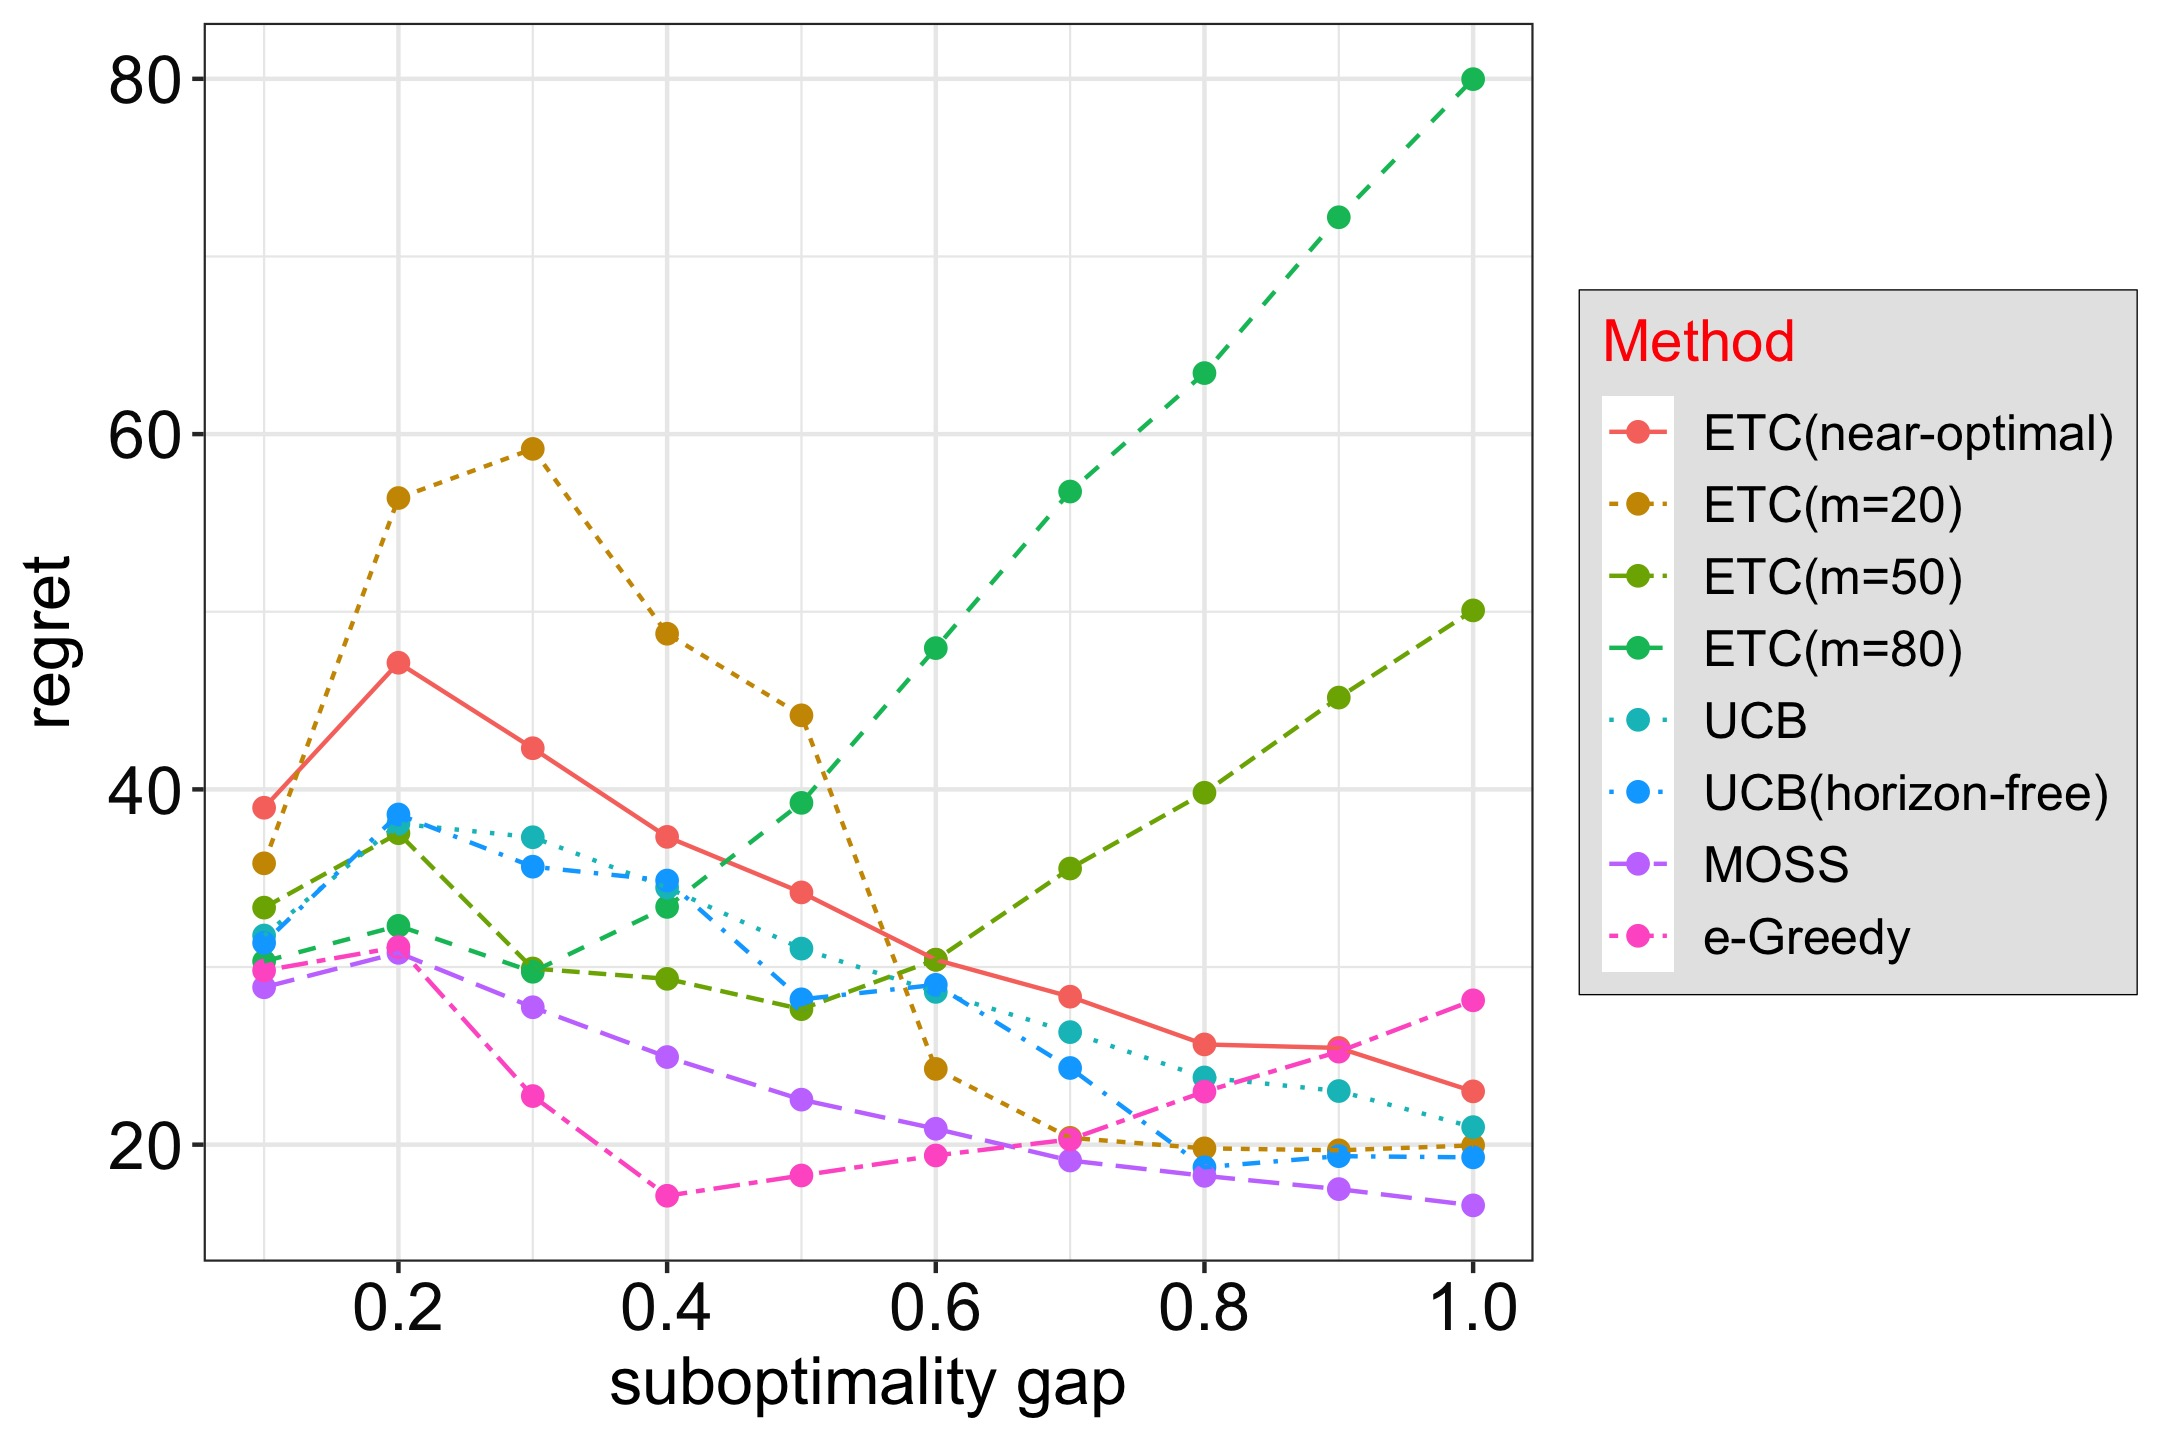
\includegraphics[width = 0.55\textwidth,clip,trim = 1cm 0cm 0cm 0cm]{sb}
%\caption{Numerical simulations of several stochastic learning policies for two-armed Gaussian bandits with varying sub-optimality gap.}
%  \label{fig:1}
%\end{figure}



\section{Lower bounds on regret}

\subsection{Minimax lower bound}

We introduce the \emph{minimax} lower bound in this section, which can help us understand the best universal behavior of stochastic bandit algorithms. Let $\V$ be the environment class consisting of the admissible $\mu$. The worst-case regret for a policy $\pi$ is defined as 
\begin{align*}
R_n(\pi, \V):=\sup_{\mu\in\V}R_n(\pi).
\end{align*}
The minimax regret $R_n^*$ is the best worst-case regret among the possible policies: 
\begin{align}
R_n^*:=\inf_{\pi}R_n(\pi, \V).\label{s:mm}
\end{align}
A good lower bound for \eqref{s:mm} will illustrate the limit in stochastic bandits learning. We introduce a natural way to approach this problem.  The general idea is to show that for any $\pi\in\Pi$, there exist two bandits $\mu, \mu'\in\V$ such that $R_{n,\mu}(\pi)$ and $R_{n,\mu'}(\pi)$ cannot be both small at the same time. Intuitively, a good instance for $\mu$ is bad for $\mu'$, and vice versa. This often implies that the $\mu$ and $\mu'$ are distant from each other in the parameter space. On the other hand, $\pi$ should not distinguish $\mu$ from $\mu'$ so that $\E_\mu\approx\E_{\mu'}$, which requires $\mu$ to be close to $\mu'$. Therefore, a trade-off position is desired.  

\begin{Th}\label{s:minimax}
Let $\V$ be the class of normalized Gaussian bandits with mean $\mu=(\mu_i)_{i\in [k]}\in [0,1]^k$. Suppose that $n\geq k-1$. Then for any policy $\pi$ there exists some $\mu\in\V$ such that
\begin{align}
R_{n,\mu}(\pi)\geq\frac{1}{27}\sqrt{(k-1)n}. \label{s:6}
\end{align}  
\end{Th}

There are several ways to prove this theorem. Here we describe two of them inspired from the Le Cam's method and the Assouad's method, which are standard techniques in the minimax theory of statistics, see \cite{Yu_1997}. 


\begin{proof}[~Proof based on Le Cam's method]
Fix a policy $\pi$. Let $\Delta\in [0, 1/2]$ be some parameter to be tuned later. Consider two bandits defined as
$\mu = (\Delta, 0, \cdots, 0)$ and $\mu = \mu'$ except at $i$, where $\mu_i = 2\Delta$, and $i$ is the least-played arm in $\mu$ on average: $i=\arg\min_{j>1}\E_\mu[T_j(n)]$. Using the Chebyshev inequality,
\begin{align}
R_{n, \mu}(\pi)+R_{n, \mu'}(\pi)\geq \frac{n\Delta}{2}\left(\P_\mu\left(T_1(n)\leq \frac{n}{2}\right)+\P_{\mu'}\left(T_1(n)> \frac{n}{2}\right)\right).\label{s:3}
\end{align}
The right-hand side of \eqref{s:3} can be bounded via the Bretagnolle-Huber inequality \footnote{The Bretagnolle-Huber inequality states that for two probability measures $\P$ and $\Q$ on the same probability space $(\Omega, \mathcal{F})$, and $A\in\mathcal{F}$, 
\begin{align}
\P(A)+\Q(A^c)\geq\frac{1}{2}e^{-\min\{\textsf D_{KL}(\P, \Q), \textsf D_{KL}(\Q, \P)\}},\label{s:4}
\end{align}
where $\textsf D_{KL}(\cdot, \cdot)$ is the KL-divergence.}. 
Set $A = \{T_1(n)\leq n/2\}$ and one has 
\begin{align*}
R_{n, \mu}(\pi)+R_{n, \mu'}(\pi)\geq\frac{n\Delta}{4}e^{-\mathsf D_{KL}(\P_\mu, \P_{\mu'})}\geq\frac{n\Delta}{4}e^{-\frac{2n\Delta^2}{k-1}},
\end{align*}
where the second inequality follows from 
\begin{align}
\textsf D_{KL}(\P_\mu, \P_{\mu'})& = \sum_{j\in [k]}\E_\mu[T_j(n)]\textsf D_{KL}(\mu_j, \mu'_j)\label{s:5}= \E_\mu[T_i(n)]\textsf D_{KL}(\mu_i, \mu'_i)\leq\frac{2n}{k-1}\Delta^2.
\end{align}
Taking $\Delta = \sqrt{(k-1)/4n}$ yields the desired result. 
\end{proof}

The constant $1/27$ in the bound \eqref{s:6} can be improved to $1/9$ via Assouad's method when $k\geq 3$: 

\begin{proof}[~Proof based on Assouad's method]
Instead of considering only two arms as in the previous proof, we consider $k$ arms that are mutually inconsistent. Let $\Delta<1$ be a constant to be determined later. Let $\mu^{(0)}\in\mathcal E$ be the all-zero vector and for $i\in [k]$, define $\mu^{(k)}$ as the vector that is $\Delta$ at $i$ and $0$ elsewhere. Comparing $\mu^{(i)}$ to $\mu^{(0)}$ using the Pinsker's inequality\footnote{The Pinsker's inequality states that for two probability measures $\P$ and $\Q$ on the same probability space $(\Omega, \mathcal{F})$, their total-variation distance ($\delta(\cdot, \cdot)$) is bounded by their KL-divergence ($\textsf D_{KL}(\cdot, \cdot)$), 
\begin{align}
\delta (\P, \Q)\leq\sqrt{\frac{1}{2}\min\{\textsf D_{KL}(\P, \Q), \textsf D_{KL}(\Q, \P)\}}. \label{s:pinsker}
\end{align}} 
\begin{align*}
\frac{1}{n}\left(\E_{\mu^{(i)}}[T_i(n)]-\E_{\mu^{(0)}}[T_i(n)]\right)\leq 2\delta(\P_{\mu^{(i)}}, \P_{\mu^{(0)}})\leq\sqrt{\textsf D_{KL}(\P_{\mu^{(i)}}, \P_{\mu^{(0)}})}=\sqrt{\frac{\Delta^2}{2}\E_{\mu^{(0)}}[T_i(n)]}. 
\end{align*}
Summing over $i$ together with Jensen's inequality yields
\begin{align*}
\sum_{i\in [k]}\E_{\mu^{(i)}}[T_i(n)]\leq n+n\sqrt{\frac{\Delta^2}{2}nk}. 
\end{align*}
Therefore,
\begin{align*}
\max_{i\in [k]}R_{n, \mu^{(i)}}(\pi)\geq\frac{1}{k}\sum_{i\in [k]}R_{n, \mu^{(i)}}(\pi)\geq \Delta\left(n-\frac{1}{k}\sum_{i\in [k]}\E_{\mu^{(i)}}[T_i(n)]\right)\geq n\Delta\left(\frac{k-1}{k}-\sqrt{\frac{n\Delta^2}{2k}}\right). 
\end{align*}
Taking $\Delta=\sqrt{k/2n}$ completes the proof. 
\end{proof}


\subsection{Instance-dependent lower bound}

We consider instance-dependent lower bound for policies which are known to be `good'. First of all, let us clarify what we mean by a good policy. A policy $\pi$ is \emph{consistent} over $\V$ if for all $\mu\in\V$ and $p>0$, 
\begin{align*}
\lim_{n\rightarrow\infty}\frac{R_{n, \mu}(\pi)}{n^p} = 0. 
\end{align*}
Roughly speaking, the regret of a consistent policy is less than polynomial growth. Denote by $\Pi_{c}(\V)$ the set of consistent policies over $\V$. Assuming that $\v$ is unstructured, the following theorem suggests that the best one can hope for consistent policies is logarithmic growth. 

\begin{Th}\label{s:ins}
Suppose $\V = \prod_{i\in [k]}\V_i$ and fix $\mu\in\mathcal E$. Let $i^*$ be an optimal arm.  For any $\pi\in\Pi_c(\V)$,
\begin{align}
\liminf_{n\rightarrow\infty}\frac{R_{n,\mu}(\pi)}{\log n}\geq \sum_{i: \Delta_i>0}\frac{\Delta_i}{\mathsf d_{\inf} (\mu_i, \mu_{i^*}, \V)}, 
\end{align}
where $$\mathsf d_{\inf} (\mu_i, \mu_{i^*}, \V) = \inf_{\nu\in\V: \nu_i>\mu_{i^*}}\textsf D_{KL}(\mu_i, \nu_i).$$ 
\end{Th}

\begin{proof}
By \eqref{s:2}, it suffices to prove that for $i\in [k]$ with nonzero sub-optimality gap, 
\begin{align*}
\liminf_{n\to\infty}\E_\mu[T_i(n)]\geq \frac{1}{\mathsf d_{\inf} (\mu_i, \mu_{i^*}, \V)}.
\end{align*}
To show this, fix $\e>0$. Consider $\nu\in\V$ that agrees with $\mu$ except at the $i$-th arm, which equals $\nu_i$ such that $\textsf D_{KL}(\mu_i, \nu_i) < \mathsf d_{\inf} (\mu_i, \mu_{i^*}, \V)+\e$ for some $\e>0$. Applying the Bretagnolle-Huber inequality with $A = \{T_i(n)\leq n/2\}$, 
\begin{align}
R_{n, \mu}(\pi)+R_{n, \nu}(\pi)\geq\frac{n}{2}\min\{\Delta_i, \nu_i-\mu_{i^*}\}e^{-(\mathsf d_{\inf} (\mu_i, \mu_{i^*}, \V)+\e)\E_\mu[T_i(n)]}.\label{s:7}
\end{align}
Since $\pi$ is consistent in both $\mu$ and $\nu$, for any $p>0$ and $\e>0$, there exists a sufficiently large $N$ such that for $n>N$, 
\begin{align}
R_{n, \mu}(\pi)+R_{n, \nu}(\pi)\leq \e n^p. \label{s:8}
\end{align}
Plugging \eqref{s:8} into \eqref{s:7} with some simplification yields
\begin{align*}
\E_\mu[T_i(n)]\geq\frac{\log\left(\frac{n}{2}\min\{\Delta_i, \nu_i-\mu_{i^*}\}\right)-\log\e-p\log n}{\mathsf d_{\inf} (\mu_i, \mu_{i^*}, \V)+\e}. 
\end{align*}
Dividing both sides by $\log n$ and setting $n\to\infty$, then taking $p, \e\to 0$ finishes the proof.  
\end{proof}
\begin{Rem}
Theorem \ref{s:ins} immediately implies that instance optimality when $\delta_t = (1+t\log^2 t)^{-1}$. Indeed, let $\V$ be the class of unstructured Gaussian bandits with unit variance. For any sub-optimal $i$,  $\mathsf d_{\inf} (\mu_i, \mu_{i^*}, \V)=\Delta_i^2/2$ (achieved at $\nu$ with $\nu_i$ arbitrarily close to $\mu_{i^*}$).  By Theorem \ref{s:ins}, 
\begin{align*}
\liminf_{n\rightarrow\infty}\frac{R_{n,\mu}(\pi)}{\log n}\geq 2\sum_{i: \Delta_i>0}\frac{1}{\Delta_i}. 
\end{align*}
Combining this with Remark \eqref{ins-opt} proves the instance optimality of the choice of $\delta_t$ in the algorithm. 
\end{Rem}



\section{Thompson sampling}

In this section, we introduce the Thompson sampling in the context of stochastic bandits. Thompson sampling \cite{Thompson_1933} is well acknowledged as the first bandit algorithm which is named after the Canadian entomologist William R. Thompson. 
The idea behind it is similar to the UCB, but adopts a Bayesian point of view. Assuming the bandit is selected from a parametric family according to a prior, Thompson sampling uses the posterior computed from the explored data to guide future exploration. 
Despite being simple, Thompson sampling has not received much attention in the past eight decades. One possible reason is the long-existing gap between the empirical performance and theoretical guarantee, which was recently filled by the work \cite{agrawal2012analysis} in 2012, where a frequentist-type analysis is provided for the finite-time regret.  Further works on its asymptotic optimality as well as the Bayesian regret can be found in \cite{Kaufmann_2012} and \cite{Russo_2014}, respectively. These results reinforced and further stimulated the resurgence of interest in Thompson sampling in many academic communities. Here, we will focus on some intuitive ideas behind Thompson sampling and provide an upper bound for its Bayesian regret. The discussion is based on the chapter 36 in \cite{lattimore2018bandit} and \cite{Russo_2014}. 

Let $\mathcal E$ be the class of environments. The frequentist view on stochastic bandits is that the true bandit $\mu\in\mathcal E$ is fixed and unknown. In contrast, the Bayesian perspective assumes that $\mu$ is sampled from $\mathcal E$ according to a prior $\Q$ before the game starts, that is, $\mu\sim\Q$. The additional information on $\Q$ can hopefully help us decipher the true bandit through updated posterior. Of course, conditional on $\mu$, the cumulative regret is the same as before; however, since $\mu$ is random based on our assumption on the model, it would be more natural to consider the averaged regret defined as
\begin{align}
R_{n, \BR}=\E_\Q[R_{n,\mu}],\label{br}
\end{align}
where $R_{n,\mu}$ is defined in \eqref{s:1}. \eqref{br} is referred to as the \emph{Bayesian regret}. Bayesian optimality (as opposed to the minimax optimality) is measured by the Bayesian regret. A major appeal of the Bayesian framework is that the optimal Bayesian strategy can often be described, if not always computed. This result is closely related to the Gittins indices which we will discuss in detail in chapter \ref{ch:5}.

Thompson sampling can be described as follows. Assuming data $x_{s\pi_s}$ has been observed for $s\leq t$, one can then compute the posterior distribution on $\mu$ using the prior: $\Q(\mu|x_{s\pi_s}, 1\leq s\leq t)$. Instead of directly taking the statistics of the posterior to choose $\pi_{t+1}$, one samples a new bandit according to the posterior, and set $\pi_{t+1}$ as the optimal arm in the random realization. This randomization forces exploration until the posterior is concentrated, in which case it is expected to close to $\mu$. The details of the algorithm are as follows:

\begin{algorithm}[H]
 \KwIn{$n$: horizon; $\Q$: prior distribution on the bandit}
 \KwOut{$\pi=(\pi_t)_{t\in [n]}$}
 \begin{algorithmic}[1]
 \FOR{$t = 1, \cdots, n$}
 \STATE{Sample $\nu\sim\Q( \cdot |x_{s\pi_s}, 1\leq s\leq t-1)$\footnote{\textcolor{gray}{Parameters $\mu$ may not always represent the true mean in different models. However, it is always the case that the true mean is a function (link function) of $\mu$. So in general one should sample $\nu$ from the posterior distribution of the mean. Here for simplicity, we just take the function to be identity for illustration.}}}
 \STATE{$\pi_{t} = \argmax_{i\in [k]}\nu_i$}
\ENDFOR
 \end{algorithmic}
\caption{Thompson Sampling} 
\label{alg:TS}
\end{algorithm}

Before analyzing Algorithm \ref{alg:TS}, we give some intuition why the posterior distribution is helpful for the inference of $\mu$. For convenience we assume that the bandit is unstructured. Let $f_i(x;\nu_i)$ be the density of the reward of arm $i$ with parameter $\nu_i$. For $i\in [k]$, let $n_i$ be the number of pulls on $i$, and denote the corresponding rewards as $z_{i1}, \cdots, z_{in_i}$. For convenience we may assume that $n_i$ are deterministic. In this case, the posterior distribution $p$ given the explored data is
\begin{align*}
p(\nu)\propto\Q(\nu)\prod_{i\in [k]}\prod_{t\in [n_i]}f_i(z_{it};\nu_i).
\end{align*}
Therefore, 
\begin{align*}
\log\frac{p(\mu)}{p(\nu)} &= \log\frac{\Q(\mu)}{\Q(\nu)}+\sum_{i\in [k]}\sum_{t\in [n_i]}\log\frac{f_i(z_{it};\mu_i)}{f_i(z_{it};\nu_i)}\\
& \approx \log\frac{\Q(\mu)}{\Q(\nu)}+\sum_{i\in [k]}n_i\E_{z\sim f_i(\cdot; \mu_i)}\left[\log\frac{f_i(z;\mu_i)}{f_i(z;\nu_i)}\right]\\
& =  \log\frac{\Q(\mu)}{\Q(\nu)}+\sum_{i\in [k]}n_i\mathsf D_{KL}(\mu_i, \nu_i),
\end{align*}
so that
\begin{align*}
\frac{p(\mu)}{p(\nu)} \approx \frac{\Q(\mu)}{\Q(\nu)}e^{\sum_{i\in [k]}n_i\mathsf D_{KL}(\mu_i, \nu_i)}.
\end{align*}
where $\mathsf D_{KL}(\cdot, \cdot)$ is the KL-divergence. This observation has the following consequences:
\begin{itemize}
\item When $i$ has been pulled many times, the $i$-th marginal of $p(\nu)$ is concentrated, thus encouraging future pulls to explore in other directions. When all arms have been well-explored, $p(\nu)d\nu\approx\delta_{\mu}$.

\item The convergence rate of $p(\nu)d\nu$ to $\delta_{\mu}$ would be slow if $\Q(\mu)$ is small, so the bandit in this case is hard to learn from the posterior, hence a large $R_{n,\mu}$ is expected. On the other hand, $\Q(\mu)$ being small suggests that $\mu$ is unlikely to be obtained under $\Q$. When averaging over $\Q$, $R_{n,\mu}$ should be not too large. 
\end{itemize}

These observations give some informal justification for the promising performance of Thompson sampling. The next theorem provides a rigorous upper bound for the Bayesian regret under appropriate assumptions:

\begin{Th}
In the Bayesian bandit set-up, assume that for $\nu\in\mathcal E$ and $i\in [k]$, $\nu_i$ has its mean in $[0,1]$ and is $1$-sub-gaussian after centering. Then, the Bayesian regret in the Thompson sampling is bounded by
\begin{align*}
R_{n,\BR}\leq 9\sqrt{kn\log n}. 
\end{align*}
\end{Th}

\begin{proof}
Let $i^*=\argmax_{i\in [k]}\mu_i$ and $\mathcal F_t = \sigma(\pi_1, x_{1\pi_1},\cdots, \pi_t, x_{t\pi_t})$. The Bayesian regret can be written as
\begin{align}
R_{n, \BR} = \sum_{t\in [n]}\E[\mu_{i^*}-\mu_{\pi_t}]. \label{dTS}
\end{align}
Conditional on $\mathcal F_{t-1}$, $i^*$ and $\pi_t$ have the same distribution\footnote{It should be warned that $\mu_{i^*}$ and $\mu_{\pi_t}$ have different distributions since the former is always no less than the latter.} ($\argmax$ of two conditional independent samples from the posterior). \eqref{dTS} can therefore be bounded via centralization. Fix $\delta>0$. A good choice is to use $\text{UCB}_{\pi_t}(t-1,\delta)$, which has the same distribution as $\text{UCB}_{i^*}(t-1,\delta)$ given $\mathcal F_{t-1}$.  Therefore, it follows from the tower property that
\begin{align*}
R_{n, \BR} =  \sum_{t\in [n]}\left(\E[\mu_{i^*}-\text{UCB}_{i^*}(t-1,\delta)]+\E[\text{UCB}_{\pi_t}(t-1,\delta)-\mu_{\pi_t}]\right).
\end{align*}
With probability at least $1-kn\delta$, for $i\in [k]$ and $t\in [k]$,
\begin{align*}
0\leq \text{UCB}_{i}(t-1,\delta)-\mu_{i}\leq 2\sqrt{\frac{2\log\left(\frac{1}{\delta}\right)}{T_i(t-1)}}.
\end{align*}
Therefore,
\begin{align*}
R_{n,\BR}&\leq kn^2\delta + \sum_{i\in [k]}\int_{0}^{T_{i}(n)}2\sqrt{\frac{2\log\left(\frac{1}{\delta}\right)}{x}}dx\\
&\leq kn^2\delta + \sum_{i\in [k]}\sqrt{32T_i(n)\log\left(\frac{1}{\delta}\right)}\\
&\leq kn^2\delta+\sqrt{32nk\log\left(\frac{1}{\delta}\right)},
\end{align*}
where the last step follows from Jensen's inequality. Setting $\delta=n^{-2}$ completes the proof. 
\end{proof}

\begin{Rem}
The idea of using direct sampling from posterior distributions can be further extended. 
For example, one may consider seeking an optimistic estimate for the true mean as in the UCB algorithm, which can be done by calculating the quantile of the marginal posterior for each arm. 
Such idea first appeared in \cite{kaufmann2012bayesian} and the corresponding algorithm is called the Bayes-UCB:

\begin{algorithm}[H]
\KwIn{$n$: horizon; $\Q$: prior distribution on the bandit; $c$: parameters of the quantile}
\KwOut{$\pi=(\pi_t)_{t\in [n]}$}
\begin{algorithmic}[1]
 \FOR{$t = 1, \cdots, n$}
 \FOR{$i = 1, \cdots, k$}
 \STATE{Calculate the posterior marginal $Q_{ti}$ for arm $i$ from $Q( \cdot |x_{s\pi_s}, 1\leq s\leq t-1)$}
 \STATE{$q_{ti} = \max\left\{r: \Q_{ti}\left((-\infty, r]\right)\leq 1-\frac{1}{t(\log n)^c}\right\}$} \ \ \ \  \tcp{Calculate the $(1-t^{-1}(\log n)^{-c})$-quantile for arm $i$}
\ENDFOR
\STATE{$\pi_{t} = \argmax_{i\in [k]}q_{ti}$}
\ENDFOR
 \end{algorithmic}
\caption{Bayes-UCB} 
\label{alg:B-UCB}
\end{algorithm}

Analysis of Algorithm \ref{alg:B-UCB} in the frequentist setting for Bernoulli bandits with Beta priors is given in \cite{kaufmann2012bayesian}. The idea follows from our intuition provided before but was made rigorous using the tail bounds for Beta distributions. Numerical results in the paper demonstrated a superior performance of Bayes-UCB over some other frequentist-based algorithms. It also showed that the Bayes-UCB strategy, when used with a sparsity-incuding prior, can be numerically approximated using Markov Chain Monte Carlo simulations.  

\end{Rem}


\chapter{Stochastic Linear Bandits}

\section{Some generalization}

Recall the definition of regret given in \eqref{s:1}. In many practical situations, not only is the chosen reward observed by the player but also the side information associated with it.  Such extra knowledge makes the model more complicated and as a consequence, the best possible policy in hindsight could be more optimal than the one used in \eqref{s:1}.  In this chapter, we will extend stochastic bandits to a more general class of bandit problems where side information can be appropriately included, and understand their learning strategies. The discussion closely follows the one in \cite{lattimore2018bandit}. 
As a starter, let us consider a stochastic model where contextual information is available. 

Contextual structures can be made of good use in bandit learning. Based on the classical stochastic bandit model, we further assume that players have access to the present context before selecting an arm in each round. Precisely, let $\mathcal C$ be the set of contexts and $\pi=(\pi_t)_{t\in [n]}\in [k]^n$ be a policy. $\pi_t$ is measurable with respect to the past decisions/rewards as well as the contexts revealed up to time $t$. The rewards collected by the player are 
\begin{align}
x_{t} = r(c_t, \pi_t)+\eta_{t}\ \ \ \ \ \ t\in [n],\label{sl:1}
\end{align}
where $c_t\in\mathcal C$ (deterministic or random) is the context in round $t$, $r(\cdot, \cdot):\mathcal C\times [k]\to\R$ is the reward function\footnote{The reward function, which is the mean of the reward distribution, is analogous to $\mu$ in chapter 1 but has two indices.}, and $\eta_{t}$ is the noise satisfying 
\begin{align}
\E[e^{\lambda\eta_{t}}|c_{1}, \pi_{1}, x_{1}, \cdots, c_{t}, \pi_{t}]\leq e^{\frac{\lambda^2}{2}}. \label{sl:2}
\end{align}
It is easy to check from \eqref{sl:2} that $\eta_t$ is sub-gaussian conditional on the history. \eqref{sl:1} and \eqref{sl:2} together lead to the so-called \emph{stochastic contextual bandits}. Due to the lack of knowledge of $r$, the regret is characterized by 
\begin{align}
R_n = \E\left[\sum_{c\in\mathcal C}\sum_{t: \pi_t = c}\max_{i\in [k]}r(c, i)\right] - \E\left[\sum_{t\in [n]}x_{t}\right]. \label{sl:reg}
\end{align}
The regret given in \eqref{sl:reg} implicitly agrees that the best policy in each round is to play the arm with the largest expected reward in the present context, which is most meaningful if the dependence between contexts and actions is mild. A counterexample is when an optimal action at the beginning leads to unfavorable contexts in the subsequent rounds. The ideal $c_t$ under our consideration is either deterministic or independent of the past actions.  Conditional on $(c_t)_{t\in [n]}$, $R_n$ becomes a sum of regret of $|\mathcal C|$ stochastic bandits. Heuristically, the best strategy is to treat the contexts separately and apply the optimal policy for each individual,  
\begin{align}
R_n=\E\left[\sum_{c\in\mathcal C}\E\left[R_{n,c}|c_1, \cdots, c_n\right]\right]\stackrel{\text{Thm.}\ \ref{s:minimax}}{\lesssim}\E\left[\sum_{c\in\mathcal C}\sqrt{k\sum_{t\in [n]}\mathbb I_{c_t = c}}\right]\leq\sqrt{nk|\mathcal C|}.\label{sl:3}
\end{align} 
This immediately generalizes the results in Section \ref{sec1} to the stochastic contextual bandits, assuming nothing on the reward function $r$. However, in practice, $|\mathcal C|$ can be astronomical (i.e., $|\mathcal C|>>\sqrt{n}$), making \eqref{sl:3} a vacuous bound.  The problem here is that our strategy only uses the combinatorial nature of $\mathcal C$. For example, supposing that $\mathcal C$ is a subset of a normed space and $r$ is continuous, one would expect $r(c, \cdot)$ and $r(c', \cdot)$ to be close if $||c-c'||$ is small. Yet this is not utilized in the above algorithm design which deals with elements in $\mathcal C$ in separately. To utilize other information of $\mathcal C$, we could further hypothesize on the structures of $r$ (i.e., $r$ is in some parametric family). A simple choice gives rise to a class of interesting models which we will study next. 

Suppose that $r(c,i)$ is a linear function of a high-dimensional feature determined by $(c, i)$ via a kernel map $\phi(c,i): \mathcal C\times [k]\to\R^d$. That is, $r(c, i) = \langle\t, \phi(c,i) \rangle$ for some $\t\in\R^d$. In this case \eqref{sl:reg} can be rewritten as 
\begin{align}
R_n = \E\left[\sum_{t\in [n]}\max_{a\in\mathcal A_t}\langle\theta, a\rangle-x_{t}\right],\label{sl:4}
\end{align}  
where $\mathcal A_t = \{\phi(c_t, i)\}_{i\in [k]}$ is the set of features available at time $t$. Here $\theta$ is unknown, and $\mathcal A_t$ is a finite set which can be either deterministic or random. This particular parametrization of $r$ is called \emph{stochastic linear bandits}, which will be our focus in the rest of the chapter.  One may also consider other parametrization forms of $r(c,i)$. For example, in generalized stochastic linear bandits, $r(c,i)$ is taken as the $\Phi( \langle\t, \phi(c,i) \rangle)$, where $\Phi$ is the link function, see \cite{filippi2010parametric, li2017provably}. We will briefly discuss this in a remark at the end of next section. 

We next discuss some policies in stochastic linear bandits, depending on different assumptions on $\mathcal A_t$. Note that $\mathcal A_t$ is finite from the perspective of stochastic contextual bandits and the kernel map. However, in the general set-up of stochastic linear bandits, $\mathcal A_t$ is allowed to be infinite. Regardless of varying assumptions on $\mathcal A_t$, the regret defined in \eqref{sl:4} is based on the lack of information of $r$ so that one always needs to efficiently estimate for $\theta$ in the exploration process. Nevertheless, the efficiency here can have different meanings for different types of $\mathcal A_t$, which needs to be discussed in a case-dependent manner. 

\section{Stochastic linear bandits with finite and fixed action set}

We begin our analysis for stochastic linear bandits whose action set $\mathcal A_t = \mathcal A$ does not change with time. We also assume that $|\mathcal A|=k$. Let $a_t\in\mathcal A$ be the feature vector associated with the action under some policy $\pi$ at time $t$. The exploration process suffices to estimate $\t$, and a natural estimator is the least-squares estimator. One may use the Ridge estimator if having invertibility issues. Precisely, in round $t$, $\t$ is estimated by $\hat{\t}_t$, where $\hat{\t}_t $ solves the normal equations: 
\begin{align*}
\underbrace{\begin{pmatrix}
a_1, \cdots, a_{t-1}
\end{pmatrix}}_{A^T_{t-1}}\underbrace{\begin{pmatrix}
a_1^T \\
\vdots \\
a_{t-1}^T
\end{pmatrix}}_{A_{t-1}}\t = \underbrace{\begin{pmatrix}
a_1, \cdots, a_{t-1}
\end{pmatrix}}_{A^T_{t-1}}\begin{pmatrix}
x_1 \\
\vdots \\
x_{t-1}
\end{pmatrix}.
\end{align*}
Note that the design matrix $A_{t-1}$ depends on the past actions. Since $\mathcal A$ is fixed, a good policy in the exploration stage should efficiently estimate the marginals of $\t$ along the directions in $\mathcal A$. In other words, for any $\e, \delta>0$, we wish to find a $\pi$ such that 
\begin{align}
T_{\pi}(\e, \delta):=\inf\left\{t: \max_{a\in\mathcal A}\underbrace{\P\left(|\langle\hat{\t}_t-\t, a\rangle|>\e\right)\leq\delta}_{\textcolor{black}{\text{used to build c.i. for}\ \langle\t, a\rangle}}\right\}\label{sl:5}
\end{align}
is as small as possible. This is equivalent to the optimal experimental design problem in statistics. 
To see this, note that for fixed $a\in\mathcal A$, 
\begin{align*}
\P\left(|\langle\hat{\t}_t-\t, a\rangle|>\sqrt{2||a||^2_{V_{t-1}^{-1}}\log\left(\frac{2}{\delta}\right)}\right)\leq\delta,
\end{align*}
where $V_{t-1} = A^T_{t-1}A_{t-1}$. Setting 
\begin{align*}
\sqrt{2||a||^2_{V_{t-1}^{-1}}\log\left(\frac{2}{\delta}\right)}\leq\e
\end{align*}
and solving for $t$ yields
\begin{align}
||a||_{V_{t-1}^{-1}}\leq\sqrt{\frac{\e^2}{2}\log^{-1}\left(\frac{2}{\delta}\right)}.\label{margin}
\end{align}
Since $V_t^{-1}\preceq V^{-1}_{t-1}$, an upper bound for \eqref{sl:5}, which we denote by the same notation, is
\begin{align}
T_{\pi}(\e, \delta) = \inf\left\{t: \max_{a\in\mathcal A}||a||_{V_{t-1}^{-1}}\leq \sqrt{\frac{\e^2}{2}\log^{-1}\left(\frac{2}{\delta}\right)}\right\}.\label{sl:6}
\end{align}
Let $\mathcal P(\mathcal A)$ be set of probability measures on $\mathcal A$. There is a one-to-one correspondence between policies and $\mathcal P(\mathcal A)$ asymptotically (The frequency of choosing an action $a$ in $t$ rounds under $\pi$ can be roughly viewed as the probability $p(a)$). Denote by $p$ the probability measure associated with $\pi$. It is easy to verify that 
\begin{align*}
T_{\pi}(\e, \delta) = \frac{\max_{a\in\mathcal A}||a||^2_{A^{-1}(p)}}{\frac{\e^2}{2}\log^{-1}\left(\frac{2}{\delta}\right)}+1\ \ \ \ \ A(p):=\E_p[aa^T]
\end{align*}
Hence, as $t\to\infty$, minimizing \eqref{sl:6} over the possible policies is equivalent to the following optimization problem:
\begin{align}
\min_{p\in\mathcal P(\mathcal A)}\max_{a\in\mathcal A}||a||^2_{A^{-1}(p)}.\label{sl:7}
\end{align}
The term $\max_{a\in\mathcal A}||a||^2_{A^{-1}(p)}$ is often denoted by $g(p)$, and \eqref{sl:7} is referred to as the \emph{G-optimal design problem}. \eqref{sl:7} can be solved using the following theorem due to Kiefer and Wolfowitz \cite{Kiefer_1985}:
\begin{Th}[Kiefer-Wolfowitz]\label{KW}
Let $\mathcal A\subset\R^d$ be a compact set and $\text{span}(\mathcal A)=\R^d$. Then
\begin{align*}
p^*\text{solves \eqref{sl:7}}\Longleftrightarrow p^*\in\argmax_{p\in\mathcal P(\mathcal A)}\log\det A(p)\Longleftrightarrow g(p^*) = d. 
\end{align*}
Moreover, there exists a $p^*$ such that $\text{supp}(p^*)\leq d(d+1)/2$. 
\end{Th}
\begin{Rem}
The geometric interpretation of the set $\left\{||x||_{A^{-1}(p^*)}\leq d\right\}$ based on duality is the minimum volume enclosing ellipsoid for the set $\mathcal A$. When $\mathcal A$ is convex, this is known as \emph{John's ellipsoid}.  
\end{Rem}
\begin{Rem}
According to Theorem \ref{KW}, solving the $G$-optimal design problem is the same as finding the maximizer for $\log\det A(p)$, which is a convex optimization problem and can be approximately solved via Frank-Wolfe algorithm: For $a\in\mathcal A$ and $a_k = \argmax_{a\in\mathcal A}||a||_{A^{-1}(p_k)}^2$, 
\begin{align*}
p_{k+1}(a) = \left(1-\frac{\frac{1}{d}||a_k||_{A^{-1}(p_k)}-1}{||a_k||_{A^{-1}(p_k)}-1}\right)p_k(a) + \frac{\frac{1}{d}||a_k||_{A^{-1}(p_k)}-1}{||a_k||_{A^{-1}(p_k)}-1}\mathbb I_{a=a_k}.
\end{align*}
If $p_0$ is a uniform distribution on $\mathcal A$, then $g(p_k)\leq (1+\e)d$ for $k=\mathcal O(d\log\log |\mathcal A|+d/\e)$.
\end{Rem}

Once \eqref{sl:7} is (approximately) solved, one can use the solution to construct a near-optimal policy for exploration. Algorithms in Section \ref{sec1} like ETC naturally extend to this case. However, similar problems still exist as the best trade-off point usually depends on the sub-optimality gaps. An alternative approach is to take the exploration adaptively together with a phase-elimination process, which is given below:

\begin{algorithm}[H]
 \KwIn{$\mathcal A$: action set; $\delta$: confidence level}
 \KwOut{ $(a_t)_{t\in [n]}.$}
\begin{algorithmic}[1]
\STATE \textbf{Initialization}: $\ell = 0$, $\mathcal A_1 = \mathcal A$, $T_0 = 0$, $d_0=d$ and $N_0 = 0$
 \WHILE{$N_\ell\leq n$}
\STATE $\ell = \ell + 1$
\STATE $\e_\ell = 2^{-\ell}$
 \STATE $p_\ell \in\argmax_{p\in\mathcal P(\mathcal A_\ell)}\log\det \mathcal A_\ell(p)$ and $\text{supp}(p_\ell)\leq d_{\ell-1}(d_{\ell-1}+1)/2$
\STATE $d_\ell = \min\{|\mathcal A_\ell|, d\}$.
 \FOR{$a\in\mathcal A_\ell$}
 \STATE $T_\ell(a)=\displaystyle\left\lceil 2\e_\ell^{-2}d_\ell p_\ell(a)\log\left(\frac{2k\ell(\ell+1)}{\delta}\right)\right\rceil$
 \ENDFOR
\STATE $T_\ell = \sum_{a\in\mathcal A}T_\ell(a)$
\STATE For $t\in [N_{\ell-1}+1,N_{\ell_1}+T_\ell]$ choose action $a\in\mathcal A_\ell$ $T_\ell(a)$ times. Denote the  design matrix by $A_\ell$ 
\STATE $\hat{\t}_\ell = (A^T_\ell A_\ell)^{-1}A_\ell^T(x_{T_{\ell-1}+1}\cdots, x_{T_\ell})^T$
\STATE $\mathcal A_{\ell+1} = \{a\in\mathcal A_\ell: \max_{b\in\mathcal A_\ell}\langle\hat{\t}_\ell, b-a\rangle\leq 2\e_\ell\}$ 
\STATE $N_\ell = N_{\ell-1} + T_\ell$
\ENDWHILE
\end{algorithmic}
\caption{Phase-elimination with $G$-optimal Exploration Algorithm } 
\label{alg:sl-finite}
\end{algorithm}

Assume additionally that the largest sub-optimality gap is bounded by $1$. Then the regret analysis of Algorithm \ref{alg:sl-finite} can be summarized in the following theorem:

\begin{Th}\label{sl:finite}
The psudo-regret $\bar{R}_n=n\max_{a\in\mathcal A}\langle\t, a\rangle-\sum_{t\in [n]}\langle\t, a_t\rangle$ in Algorithm \ref{alg:sl-finite} satisfies
\begin{align*}
\P\left(\bar{R}_n>4\sqrt{\left(16n\log\left(\frac{nk}{\delta}\right)+d\right)d} \right)\leq \delta, 
\end{align*}
\end{Th}
Moreover, taking $\delta=n^{-1}$ and using that $\bar{R}_n\leq n$, 
\begin{align*}
R_n\leq 4\sqrt{\left(32n\log\left(\frac{nk}{\delta}\right)+d\right)d}.  
\end{align*}
\begin{proof}
Algorithm \ref{alg:sl-finite} guarantees that with a high probability, an optimal action $a^*$ is always in $\mathcal A_\ell$ and sub-optimal arms can only survive finitely many times. In fact, 
\begin{align*}
&\P\left(a^*\in\mathcal A_\ell\  \text{for only finitely many}\ \ell \right)\\
\leq&\ \  \sum_{\ell\in\N}\P\left(a^*\notin\mathcal A_{\ell+1}|a^*\in\mathcal A_{\ell}\right)\\
\leq&\ \ \sum_{\ell\in\N}\sum_{\substack{a\in\mathcal A_\ell\\ a\neq a^*}}\left(\P\left(|\langle\hat{\t}_{\ell+1}-\t, a^*\rangle|>\e_{\ell+1}\right)+\P\left(|\langle\hat{\t}_{\ell+1}-\t, a\rangle|>\e_{\ell+1}\right)\right)\leq\frac{\delta}{k}.
\end{align*}
On the other hand, let $\Delta_a = \langle\t, a^*-a\rangle$ be the sub-optimality gap between $a$ and $a^*$ and define $\ell_a = 2+\lceil\log\Delta_\ell^{-1}\rceil$ (base 2). Then, 
\begin{align*}
\P\left(a\in\mathcal A_{\ell_a}\right)&\leq \P\left(|\langle\hat{\t}_{\ell_a}-\t, a^*\rangle|>\e_{\ell_a}\right)+\P\left(|\langle\hat{\t}_{\ell_a}-\t, a\rangle|>\e_{\ell_a}\right)\leq \frac{\delta}{k}. 
\end{align*}
Taking a union bound gives
\begin{align}
\P\left(a^*\in\bigcap_{\ell\in\N}\mathcal A_\ell\ \&\ a\notin \mathcal A_{\ell_a}\ \text{for all $a\in\mathcal A$ with $\Delta_a>0$} \right)\geq 1-\delta. \label{sl:8}
\end{align}
We now estimate $\bar{R}_n$ conditional on the event defined in \eqref{sl:8}. Let $\Delta>0$ be some parameter to be tuned later. We first consider the actions played in the first $n$ rounds with sub-optimality gap less than $\Delta$. It is clear that the cumulative loss incurred by these actions is bounded by $n\Delta$. On the other hand, the actions with sub-optimality gap greater than $\Delta$ can be played only in the first $\ell_\Delta$ rounds, where $\ell_\Delta = 1+\lceil\log\Delta^{-1}\rceil\leq 2+\log\Delta^{-1}$. The regret of these actions is bounded by the total loss incurred in the first $\ell_\Delta$ rounds of exploration, which is further bounded \footnote{Conditional on \eqref{sl:8}, the largest sub-optimality gap in the $\ell$-th round is at most $4\e_\ell$ when $\ell>1$. The same holds also for $\ell=1$ since $1\leq 4\e_1$.} by  
\begin{align*}
\sum_{\ell = 1}^{\log n\wedge \ell_\Delta}4\e_\ell T_\ell &\leq \frac{64}{\Delta}d\log\left(\frac{2k\log n}{\delta}\right) + 4d,
\end{align*} 
 Therefore, 
\begin{align*}
\bar{R}_n&\leq\inf_{0<\Delta<1}\left\{n\Delta+\frac{64}{\Delta}d\log\left(\frac{2k\log n}{\delta}\right)+4d\right\}\leq 16\sqrt{nd\log\left(\frac{2k\log n}{\delta}\right)}+4d\\
&\leq 32\left(\sqrt{nd\log\left(\frac{k\log n}{\delta}\right)}+d\right)\leq 4\sqrt{\left(16n\log\left(\frac{nk}{\delta}\right)+d\right)d}. 
\end{align*}
The proof is thus complete. 
\end{proof}
\begin{Rem}
One advantage of Algorithm \ref{alg:sl-finite} is that it behaves well even when the model is misspecified. Particularly, if the observation $x_t$ is contaminated by some noise of magnitude less than $\e$, then it can be proved that 
\begin{align*}
R_n=\mathcal O\left(\sqrt{nd\log (nk)}+\e n\sqrt{d}\log n\right). 
\end{align*}
\end{Rem}

\begin{Rem}
Algorithm \ref{alg:sl-finite} can be viewed as the generalized version of Algorithm \ref{alg:elimination} for (linear) structured stochastic bandits. The uniform exploration in each phase is replaced with an effective allocation given by the Kiefer-Wolfowitz Theorem. Indeed, Theorem \ref{sl:finite} implies Theorem \ref{elim} by taking $\mathcal A$ as canonical bases in $\R^d$ and $d=k$.  
\end{Rem}

\section{Stochastic linear bandits with general action sets}

We now consider stochastic linear bandits with general action sets, meaning that $\mathcal A_t$ can be both time-varying and infinite.
This requires us to find all-rounded confidence sets adaptively.  
Suppose for now that $\t$ is still estimated by the least-squares estimator. 
A possible choice for confidence sets is a sequence of balls weighted by the design matrices, similar to the ones used in the classical linear regression.
However, the analysis here is more intricate since the design matrix is data-dependent.  
We also provide a different approach to constructing the confidence sets based on online learning prediction, which allows one to utilize the prior knowledge of $\t$ in the construction. 
Except for the confidence sets, the general algorithm resembles the UCB algorithm in Section \ref{sec1}. 
This implies that $\t$ is estimated stepwise and the decision is made under optimistic bias. 
When the exploration data is small, the design matrix may not be invertible.  
Therefore, it is thus necessary to use regularized least-squares estimators to avoid invertibility issues (at the beginning). Particularly, let $\lambda>0$ be a regularization parameter and our estimation for $\t$ at time $t$ is given by 
\begin{align}\label{est}
\hat{\t}_t = (\underbrace{\lambda I +A^T_{t-1}A_{t-1}}_{V_{t-1}(\lambda)})^{-1}A^T_{t-1}\begin{pmatrix}
x_1 \\
\vdots \\
x_{t-1}
\end{pmatrix}.
\end{align}
Suppose that the confidence set at $t$ is an $V^{-1}_{t-1}(\lambda)$-weighted ball centered at $\hat{\t}_t$\footnote{Taking $\hat{\t}_t$ as the regularized least-squares estimator is convenient and gives heuristics on the shape of the confidences sets. Other reasonable estimators also work in the following analysis.}, i.e., $\mathcal C_t = \{z\in\R^d: ||z-\hat{\t}_t||^2_{V_{t-1}(\lambda)}\leq\beta_t\}$, where $\beta_t\geq 1$ is an increasing sequence computed from $\mathcal A_1, a_1, x_1, \cdots, A_{t-1}, a_{t-1}, x_{t-1}$. Suppose also that for fixed $n$ and $\delta$, the choice of $\beta_t$ makes $\mathcal \{\mathcal C_t\}_{t\in [n]}$ form a uniform \footnote{The reason why one needs uniform confidence sets is because the algorithm is built adaptively so that estimations at different steps are different.} $(1-\delta)$-confidence set:
\begin{align}
\P(\t\in\cap_{t=1}^n\mathcal C_t)\geq 1-\delta.\label{sl:9}
\end{align} 
Practicality of \eqref{sl:9} will be justified in a moment. A version of the UCB algorithm for stochastic linear bandits can then be described as follows:

\begin{algorithm}[H]
 \KwIn{$\{\mathcal A_t\}_{t\in [n]}$: action sets; $\delta$: confidence level; $\lambda$: regularization parameter}
 \KwOut{ $(a_t)_{t\in [n]}$}
\begin{algorithmic}[1]
\STATE  \textbf{Initialization}: $t=1$, $V_1(\lambda) = \lambda I$ and $a_1\in\mathcal A_1$
 \WHILE{$t\leq n$}
\STATE $\hat{\t}_{t+1} = V^{-1}_{t}(\lambda)A_{t}^T(x_1, \cdots, x_{t})^T$
%\STATE $\beta_{t+1}=\beta_{t+1}(\mathcal A_1, a_1, x_1, \cdots, A_{t}, a_{t}, x_{t})$
\STATE $\mathcal C_{t+1} = \{z\in\R^d: ||z-\hat{\t}_{t+1}||^2_{V_{t}(\lambda)}\leq\beta_{t+1}\}$
\STATE $a_{t+1} \in \argmax_{a\in\mathcal A_{t+1}}\sup_{z\in\mathcal C_{t+1}}\langle z, a\rangle$
\STATE $V_{t+1}(\lambda) = V_{t}(\lambda)+a_{t+1}a_{t+1}^T$ 
\STATE $t = t +1$
\ENDWHILE
\end{algorithmic}
\caption{UCB Algorithm for Stochastic Linear Bandits (LinUCB)} 
\label{alg:sl-UCB}
\end{algorithm}

Algorithm \ref{alg:sl-UCB} is also known as Linear Reinforcement Learning (LinRel)\cite{dani2008stochastic, Rusmevichientong_2010}. Before discussing in detail how $\beta_t$'s are chosen, we give a general result on the asymptotic regret that Algorithm \ref{alg:sl-UCB} can achieve, as summarized in the following theorem:

\begin{Th}
Assume that for some $L>0$, 
\begin{align}
\sup_{a\in\cup_{t\in\N}\mathcal A_t}\left\{|\langle\t, a\rangle|, \frac{||a||_2}{L}\right\}\leq 1. \label{sl:10}
\end{align}
\end{Th}
For convenience we also assume that $\mathcal A_t$ is closed. Then, with probability at least $1-\delta$, the pseudo-regret $\bar{R}_n=\sum_{t\in [n]}\sup_{a\in\mathcal A_t}\langle\t, a-a_t\rangle$ in Algorithm \ref{alg:sl-UCB} satisfies that
\begin{align}
\bar{R}_n\leq 2+\sqrt{8n\beta_n\log\left(\frac{\det V_n(\lambda)}{\det V_1(\lambda)}\right)}\leq 2+\sqrt{8dn\beta_n\log\left(\frac{d\lambda+nL^2}{d\lambda}\right)}. \label{sl:11}
\end{align}
\begin{proof}
It suffices to check that \eqref{sl:11} holds on the event defined in \eqref{sl:9}. The assumptions in the theorem imply that $\mathcal A_t$ is compact thus there exists $z_t\in\mathcal C_t$ such that $\langle z_t, a_t\rangle = \sup_{z\in\mathcal C_t}\langle z, a_t\rangle$. Then,
\begin{align*}
\bar{R}_n& = \sum_{t\in [n]}\sup_{a\in\mathcal A_t}\langle\t, a-a_t\rangle\stackrel{\eqref{sl:10}}{\leq} 2+ \sum_{t=2}^n\min\left\{\underbrace{\left(\sup_{a\in\mathcal A_t}\langle\t, a\rangle-\langle z_t, a_t\rangle\right)}_{\leq 0 \ \text{ on}\ \eqref{sl:9}}+\langle z_t-\t, a_t\rangle, 2\right\}\\
&\stackrel{\eqref{sl:9}}{\leq} 2+2\sum_{t=2}^n \min\left\{\sqrt{\beta_t}||a_t||_{V^{-1}_{t-1}(\lambda)}, 1\right\}\stackrel{\beta_t\leq\beta_n}{\leq} 2+2\sum_{t=2}^n \min\left\{\sqrt{\beta_n}||a_t||_{V^{-1}_{t-1}(\lambda)}, 1\right\}\\
&\stackrel{\beta_n\geq 1}{\leq} 2+2\sqrt{n\beta_n\sum_{t=2}^n\min\left\{||a_t||^2_{V^{-1}_{t-1}(\lambda)}, 1\right\}}\leq 2+2\sqrt{2n\beta_n\sum_{t=2}^n\log \left(1+||a_t||^2_{V^{-1}_{t-1}}\right)},
\end{align*} 
where the last step uses the inequality $\min\{1, u\}\leq 2\log(1+u)$ for $u\geq 0$. Since $V_t$ is obtained from $V_{t-1}$ through a rank-1 update, it is easy to check that $$\prod_{t=2}^n \left(1+||a_t||^2_{V^{-1}_{t-1}}\right)=\frac{\det V_n(\lambda)}{\det V_1(\lambda)}.$$Plugging this into the above estimate completes the proof of the first part in \eqref{sl:11}. The second part follows immediately by noting that $\det V_n(\lambda)\leq (\text{tr}(V_n(\lambda))/d)^d\leq (\lambda + nL^2/d)^d$.
\end{proof}
\begin{Rem}
The constant $2$ comes from exploring the first action arbitrarily. It does not affect the asymptotic result and will be omitted later for convenience. 
\end{Rem}

\begin{Rem}\label{2.9}
The above proof shows that how $\t$ is estimated in \eqref{est} does not really matter, as long as the confidence set is weighted by $V_{t-1}$ (where $V_{t-1}$ is updated in the rank-1 manner) and centered at the estimation. One may use other reasonable estimators in both theoretical analysis and practice, see section \ref{sec:olp}. 
\end{Rem}

\begin{Rem}[Generalized stochastic linear bandits]
Similar idea could be extended to generalized stochastic linear bandits. Suppose that the conditional reward of an action $a$ is given by $\Phi(\langle a, \t\rangle)$, where $\Phi$ is the link function. In this case, $\t$ could be estimated by the quasi-maximum likelihood estimate\footnote{This is the true maximum likelihood estimate under appropriate exponential family assumptions.} $\hat{\t}_{t+1}$:
\begin{align}
\sum_{s\in [t]}\left(x_t-\Phi(\langle a_t, \hat{\t}_{t+1}\rangle)\right)a_t = 0. \label{qsm}
\end{align}
However, in order to apply Algorithm \ref{alg:sl-UCB} one needs to obtain confidence sets as in \eqref{sl:9}, which is difficult for the MLE in practice. 
An alternative approach, as observed in \cite{filippi2010parametric}, is that the solution to the optimization in step $5$ in Algorithm \ref{alg:sl-UCB} is equivalent to $\argmax_{a\in\mathcal A_{t+1}}\Phi(\langle a, \hat{\t}_{t+1}\rangle)+\sqrt{\beta_ {t+1}}||a||_{V_t^{-1}(\lambda)}$ when $\Phi$ is identity. This leads to the so-called UCB-GLM algorithm, which is given below:

\begin{algorithm}[H]
 \KwIn{$\{\mathcal A_t\}_{t\in [n]}$: action sets; $\beta_t$: exploration parameter; $\lambda$: regularization parameter}
 \KwOut{ $(a_t)_{t\in [n]}$}
\begin{algorithmic}[1]
\STATE  \textbf{Initialization}: $t=1$, $V_1(\lambda) = \lambda I$ and $a_1\in\mathcal A_1$
 \WHILE{$t\leq n$}
\STATE Solve \eqref{qsm} for $\hat{\t}_{t+1}$
%\STATE $\beta_{t+1}=\beta_{t+1}(\mathcal A_1, a_1, x_1, \cdots, A_{t}, a_{t}, x_{t})$
\STATE $a_{t+1} \in \argmax_{a\in\mathcal A_{t+1}}\Phi(\langle a, \hat{\t}_{t+1}\rangle)+\sqrt{\beta_ {t+1}}||a||_{V_t^{-1}(\lambda)}$
\STATE $V_{t+1}(\lambda) = V_{t}(\lambda)+a_{t+1}a_{t+1}^T$ 
\STATE $t = t +1$
\ENDWHILE
\end{algorithmic}
\caption{UCB-GLM Algorithm} 
\label{alg:sl-UCB-GLM}
\end{algorithm}
The specific choice for $\beta_t$ with theoretical guarantee can be found in \cite{filippi2010parametric, li2017provably}. The penalty term can be viewed as the variance, so that exploration is encouraged when the variance is large. 
\end{Rem}

\begin{Rem}[Thompson sampling for stochastic linear bandits]
Thompson sampling can also be used for stochastic linear bandits. Assuming that the true parameter is generated from some distribution $\Q$, then the algorithm can be described as follows:

\begin{algorithm}[H]
 \KwIn{$n$: horizon; $\Q$: prior distribution on the bandit}
 \KwOut{$(a_t)_{t\in [n]}$}
 \begin{algorithmic}[1]
 \FOR{$t = 1, \cdots, n$}
 \STATE{Sample $\t\sim\Q( \cdot |a_s, x_{s}, 1\leq s\leq t-1)$}
 \STATE{$a_{t} = \argmax_{a\in \mathcal A_{t}}\langle\t, a\rangle$}
\ENDFOR
 \end{algorithmic}
\caption{Thompson Sampling for Linear Bandits} 
\label{alg:TSL}
\end{algorithm}
A major advantage of Thompson sampling over frequentist based methods is the computational convenience. 
\end{Rem}

We next give two ways of finding valid $\beta_t$'s to achieve \eqref{sl:9}, both of which used the maximal inequality for self-normalized martingales. 

\subsection{Laplace's method}

Define $S_t = A_{t}^T(\eta_1, \cdots, \eta_t)^T$. Note that for $t\in [n]$, 
\begin{align}
||\hat{\t}_t -\t||_{V_{t-1}(\lambda)}&=\langle V^{-1}_{t-1}(\lambda)(\lambda\t - S_{t-1}), \lambda\t - S_{t-1}\rangle^{1/2}\nonumber= ||\lambda\t - S_{t-1} ||_{V^{-1}_{t-1}(\lambda)}\\
&\leq  \lambda ||\t||_{V^{-1}_{t-1}(\lambda)} + ||S_{t-1} ||_{V^{-1}_{t-1}(\lambda)}\stackrel{V^{-1}_{t-1}(\lambda)\preccurlyeq\lambda^{-1}I}{\leq} \sqrt{\lambda} ||\t||_2 + ||S_{t-1} ||_{V^{-1}_{t-1}(\lambda)}\label{sl:12}. 
\end{align}
Therefore it suffices to obtain a high-probability bound for $||S_{t-1} ||_{V^{-1}_{t-1}(\lambda)}$. The weight factor  is given by the inverse of $V_{t-1}(\lambda)$ which can be difficult to analyze. To get around we rewrite $\frac{1}{2}||S_t||^2_{V^{-1}_{t}(\lambda)}$ using the Legendre transform:
\begin{align*}
\frac{1}{2}||S_t ||^2_{V^{-1}_{t}(\lambda)} = \max_{x\in\R^d}\left(\langle x, S_t\rangle - \frac{1}{2}\langle x, x\rangle_{V_t(\lambda)}\right).
\end{align*}
Thanks to the sub-gaussian assumption on the noise, for fixed $x$, $M_t(x)=e^{\langle x, S_t\rangle - \frac{1}{2}\langle x, x\rangle_{V_t(\lambda)}}$ is a non-negative supermartingale started at $e^{-\lambda ||x||_2^2/2}$. This raises hope for a uniform bound in $t$ (as desired in \eqref{sl:9}) by appealing to the maximal inequality. However, there is an extra maximum over $x$ which needs to be addressed first. For this we use a technique called self-normalization. Self-normalization is similar to Laplace's method in asymptotic analysis.  
Note that $||\lambda\t + S_{t-1} ||_{V^{-1}_{t-1}(\lambda)}$ grows to infinity as $t\to\infty$ (otherwise there is no need to do the analysis here!).  For large $t$, if one wants to understand $\max_{x\in\R^d}\log M_t(x)$, one may study $$\bar{M}(x):=\log\int_{x\in\R^d}M_t(x)p(x)dx$$ instead, where $p(x)$ is some finite-measure whose support contains $\argmax_{x\in\R^d} M_t(x)$. 
On the other hand, if $p(x)$ is a probability measure, averaging over $x$ preserves the martingale property so that $\bar{M}(t)$ is also a non-negative supermatingale. Take $p(x)$ as a gaussian measure on $\R^d$ with covariance matrix $\lambda^{-1} I$. Then,
\begin{align*}
\bar{M}_t = \left(\frac{\lambda^d}{\det (\lambda I+V_t(\lambda))}\right)^{1/2}e^{\frac{1}{2}||S_t||^2_{(\lambda I+V_t(\lambda))^{-1}}}\geq  \left(\frac{\lambda^d}{\det (2V_t(\lambda))}\right)^{1/2}e^{\frac{1}{4}||S_t||^2_{V^{-1}_t(\lambda)}}.
\end{align*}
By Doob's maximal inequality for non-negative supermartingales, 
\begin{align*}
&\P\left(\sup_{t\in\N}||S_t||_{V^{-1}_t(\lambda)}\geq 2\sqrt{\log\left(\frac{1}{\delta}\right)+\frac{1}{2}\log\left(\frac{\det V_t(\lambda)}{\lambda^d}\right)}\right)\\
\leq&\ \P\left(\sup_{t\in\N}\log\bar{M}_t\geq\log\left(\frac{1}{2^{d/2}\delta}\right)\right) = \P\left(\sup_{t\in\N}\bar{M}_t\geq \frac{1}{2^{d/2}\delta}\right)\leq 2^{d/2}\delta\E[\bar{M}_0]=\delta. 
\end{align*}
This together with \eqref{sl:12} implies that $\beta_t$ in \eqref{sl:9} can be chosen as 
\begin{align}
\sqrt{\beta_t} &= \sqrt{\lambda}||\t||_2+2\sqrt{\log\left(\frac{1}{\delta}\right)+\frac{1}{2}\log\left(\frac{\det V_t(\lambda)}{\lambda^d}\right)}\nonumber\\
&\leq\sqrt{\lambda}||\t||_2+2\sqrt{\log\left(\frac{1}{\delta}\right)+\frac{d}{2}\log\left(\frac{d\lambda+nL^2}{d\lambda}\right)}\label{sl:13}.
\end{align}
Assuming $||\t||_2\leq\mathcal O(\sqrt{d})$, plugging \eqref{sl:13} into \eqref{sl:11} and integrates the tail probability yields that 
\begin{align*}
R_n = \mathcal O \left(d\sqrt{n}\log (nL)\right).
\end{align*}

\subsection{Online learning prediction}\label{sec:olp}

Algorithm \ref{alg:sl-UCB} (with $\hat{\t}_t$ being treated as a general estimator) is closely related to the problem of online learning prediction. 
In online learning prediction, given an action, the learner predicts the reward using some predictor built from the history before observing the reward. 
The true reward is then fed back to the learner to update the predictor. 
In the following we will use $\hat{x}_t$ as the predicted reward at time $t$, with its accuracy is measured by the cumulative squared-loss $\sum_{t\in [n]}(\hat{x}_t-x_t)^2$. 
In Algorithm \ref{alg:sl-UCB}, one still has the predictor beforehand. What makes it different is the goal of learning. One needs to decide on their own which action to play and the way how this is done is by computing multiple predicted values using appropriate confidence sets. 

In linear stochastic bandits, the best theoretic predictor is given by the expected reward function. For any predictor $\hat{x}_t$, define the regret of $\hat{x}_t$ relative to a linear predictor $z\in\R^d$ as
\begin{align*}
\rho_n(z) = \sum_{t\in [n]}(\hat{x}_t-x_t)^2-\sum_{t\in [n]}(\langle z, a_t\rangle-x_t)^2,
\end{align*}
where $a_t$ are given (either by a policy or some mysterious person). For any prior knowledge on $z$ such that $z\in\Theta\subset\R^d$, we say that the learner enjoys guarantee $B_n$\footnote{$B_n$ is a random quantity depending on data.} on $\Theta$ if $\sup_{z\in\Theta}\rho_n(z)\leq B_n$. As we will see, $B_n$ plays a crucial role in our construction of confidence sets, and allows some side-information on $\Theta$ to be incorporated.  

From now on we assume that $\hat{x}_t$ is given to estimate the reward. For example, in Algorithm \ref{alg:sl-UCB} $\hat{x}_t (\cdot)= \langle\hat{\t}_t, \cdot\rangle$. Since the confidence sets ask for an estimate for the mean reward, for any sequence of actions $(a_t)_{t\in [n]}$, we consider $Q_n := \sum_{t\in [n]}(\hat{x}_t-\langle\t, a_t\rangle)^2$. Using the Cosine theorem,  
\begin{align*}
Q_n&=\rho(\t)+2\sum_{t\in [n]}\eta_t(\hat{x}_t-\langle\t, a_t\rangle)\leq B_n+2\underbrace{\sum_{t\in [n]}\eta_t(\hat{x}_t-\langle\t, a_t\rangle)}_{\texttt{m}_n}.
\end{align*}
To further bound $Q_n$ uniformly for $n\in\N$, observe that $e^{x\texttt{m}_t-\frac{x^2}{2}Q_t}$ is a non-negative supermartingale for every $x\in\R$. Using a similar self-normalization trick as in the previous analysis and setting $x = 1$ yields that 
\begin{align}
\P\left(\forall t\in\N \ \text{s.t.}\  |\texttt{m}_t|\leq\sqrt{(1+Q_t)\log\left(\frac{1+Q_t}{\delta^2}\right)} \right)\geq 1-\delta. \label{sl:14}
\end{align}
Conditional on the event defined in \eqref{sl:14}, for every $t\in\N$, 
\begin{align*}
Q_t\leq B_t + 2\sqrt{(1+Q_t)\log\left(\frac{1+Q_t}{\delta^2}\right)},
\end{align*}
which implies
\begin{align}
Q_t\leq 1+2B_t+32\log\left(\frac{\sqrt{8}+\sqrt{1+B_t}}{\delta}\right).\label{sl:15}
\end{align}
Although \eqref{sl:15} is a confidence set, it may be unbounded and does not fit into the form used in Algorithm \ref{alg:sl-UCB}. To solve this, we restrict the confidence sets to a ball $B(L)$ of radius $L$ using \eqref{sl:10} , then identify an estimator for $\t$ based on the given predictor $\hat{x}_t$ and derive a confidence set around it. Let $\tilde{\t}_t$ be the regularized least-squares solution for the predicted values:
\begin{align*}
\tilde{\t}_t = V_t^{-1}(\lambda)A_t^T\underbrace{\begin{pmatrix}
\hat{x}_1\\
\vdots\\
\hat{x}_t
\end{pmatrix}}_{\hat{X}_t}.
\end{align*}
We can then rewrite $Q_t+\lambda ||\t||_2^2$ as 
\begin{align*}
&||A_t\t-A_t\tilde{\t}_t+A_t\tilde{\t}_t-\hat{X}_t||_2^2 + \lambda ||\t||_2^2\\
=&\  ||\t-\tilde\t_t||^2_{V_t(\lambda)} -\lambda ||\t-\tilde\t_t||_2^2 + ||A_t\tilde{\t}_t-\hat{X}_t||_2^2+2\langle\t-\tilde\t_t, \tilde\t_t\rangle_{V_t(\lambda)}\\
&\ -2\lambda \langle \t-\tilde \t_t, \tilde\t_t\rangle-2\langle\t-\tilde\t_t, \tilde\t_t\rangle_{V_t(\lambda)}+\lambda ||\t||_2^2\\
=&\ ||\t-\tilde\t_t||^2_{V_t(\lambda)}+ ||A_t\tilde{\t}_t-\hat{X}_t||_2^2+\lambda ||\tilde\t_t||_2^2.
\end{align*} 
It is then clear that 
\begin{align*}
&\left\{z\in\R^d\cap B(L): Q_t\leq 1+2B_t+32\log\left(\frac{\sqrt{8}+\sqrt{1+B_t}}{\delta}\right) \right\}\\
\subset&\ \left\{z\in\R^d: Q_t +\lambda ||z||_2^2\leq 1+2B_t+32\log\left(\frac{\sqrt{8}+\sqrt{1+B_t}}{\delta}\right) +\lambda L^2\right\}\\
\subset&\ \underbrace{\left\{z\in\R^d: ||\t-\tilde\t_t||^2_{V_t(\lambda)}\leq \underbrace{1+2B_t+32\log\left(\frac{\sqrt{8}+\sqrt{1+B_t}}{\delta}\right)+\lambda L^2}_{\beta_{t+1}} \right\}}_{\mathcal C_{t+1}}. 
\end{align*}
This together with \eqref{sl:11} implies that 
\begin{align*}
R_n = \mathcal O \left(\sqrt{nd(\E[B_n]+L^2)\log(nL)}\right)\stackrel{\text{if}\ L=\mathcal O(1)}{=}\left(\sqrt{nd\E[B_n]\log(nL)}\right).
\end{align*}
If $\t$ is known to be $s$-sparse, we can take $\Theta = \{z\in\R^d: ||z||_0\leq s\}$. In this case, it can be shown that $\E[\beta_n] \lesssim s\log n$. Hence we have $R_n = \mathcal O \left(\sqrt{nds\log^2(nL)}\right)$.
\begin{Rem}
When building up the confidence sets in the sparsity case, one needs to know the sparsity level in advance, which determines the choice for $B_t$. 
\end{Rem} 



\section{Application of stochastic linear bandits on graphs}
An interesting application of stochastic linear bandits in graph learning is the spectral bandit model \cite{valko2014spectral}. 
Other related models will be summarized in the final remark at the end of this section. 
Let $G=(V, E)$ be an undirected graph with $d$ vertices. 
For convenience, we write $V=[d]$. 
Let $\mathcal W, \mathcal D\in\R^{d\times d}$ be the similarity matrix and degree matrix, respectively. 
The unnormalized Laplacian of $G$ is defined as $\mathcal L=\mathcal D-\mathcal W$. 
In a social network represented by $G$, $\mathcal W$ measures the connections between the nodes and $\mathcal L$ measures the network diffusion dynamics. 
To formulate a bandit learning problem, we assume that $V$ is the complete action set.
At each step $t$, a subset $V_t\subset V$ is selected for the player to choose actions from.
This should be differentiated from the model where players are assigned with a node and he/she needs to choose an action from the given context \cite{cesa2013gang}.  
The expected reward by pulling $i$ is given by $r_i$, with its fluctuation charactered by a $1$-sub-gaussian distribution. 
As before, the goal is to find a strategy such that after some time $n$, the cumulative regret (which is defined in \eqref{sl:4}) is small.  
Without further assumption, this problem is nothing but a $d$-armed bandits with time-varying action sets, which can be effectively tackled using Algorithm \ref{alg:sl-UCB}\footnote{One can think of $r\in\R^d$ and node $i$ corresponds to the canonical vector $e_i\in\R^d$. }. 

In many practical situations, however, the topological properties of $G$ dictate the potential shape of $r$. 
For example, a smoothness assumption requires that $r$ changes smoothly within the clusters of $V$, which are depicted by the spectrum of $\mathcal L$.  
To incorporate such information, we hypothesize that $r$ is a \emph{smooth graph function}, which states that large components of the eigen-representation of $r$ under $\mathcal L$ are concentrated on the left end of the spectrum. 
Precisely, let $\mathcal L = Q\Lambda Q^T$ be the eigen-decomposition of $\mathcal L$, where $\Lambda = \text{diag}(\lambda_1, \cdots, \lambda_d)$ with $0=\lambda_1\leq\cdots\lambda_d$, and $Q = (q^{(1)}, \cdots,  q^{(d)})$. Then $r$ can be written as 
\begin{align*}
r =\sum_{i\in [d]}\t^{(i)}q^{(i)}\ \ \ \ \ \ \ \ \ \t^{(i)} = \langle r, q^{(i)}\rangle\ \text{for}\ i\in [d],
\end{align*}
and for $i\in [d]$,
\begin{align*}
r_i = \langle\t, \bar{q}^{(i)}\rangle\ \ \ \ \ \ \ \ \ \t = (\t^{(1)},\cdots, \t^{(d)})^T,
\end{align*}
where $\bar{q}^{(i)}$ is the $i$-th row vector of $Q$. 
The smoothness assumption on $r$ can be stated as $||r||_{\Lambda}$ being small. Since $||\cdot||_\Lambda$ is not a well-defined norm ($\lambda_1=0$), we therefore consider $||r||_\Gamma$ where $\Gamma = \Lambda +\lambda I$ for some small $\lambda>0$. 
Let $\mathcal A$ be the set of row vectors of $Q$. The smoothness assumption is equivalent to estimating $\t$ via a ridge estimator penalized by an anisotropic norm term:
\begin{align}\label{estt}
\hat{\t}_t = (\underbrace{\Gamma +A^T_{t-1}A_{t-1}}_{V_{t-1}(\lambda)})^{-1}A^T_{t-1}\begin{pmatrix}
x_1 \\
\vdots \\
x_{t-1}
\end{pmatrix}.
\end{align}
\eqref{estt} combined with Algorithm \ref{alg:sl-UCB} lead to the so-called Spectral UCB algorithm, which is stated below: 


\begin{algorithm}[H]
 \KwIn{$\mathcal L$: Laplacian matrix of the graph; $n$: horizon; $\lambda$: regularization parameter; $\delta$: confidence level}
 \KwOut{ $(a_t)_{t\in [n]}$}
\begin{algorithmic}[1]
\STATE Compute the eigen-decomposition of $\mathcal L$: $\mathcal L = Q\Lambda Q^T$ (with eigenvalues arranged in increasing order). Let $\mathcal A$ denote the set of row vectors in $Q$. 
\STATE  \textbf{Initialization}: $t=1$, $V_1(\lambda) = \lambda I+\Lambda$ and $a_1\in\mathcal A_1$
 \WHILE{$t\leq n$}
 \STATE Receive the action set $\mathcal A_{t+1}\subset\mathcal A$ in round $t+1$
\STATE $\hat{\t}_{t+1} = V^{-1}_{t}(\lambda)A_{t}^T(x_1, \cdots, x_{t})^T$
\STATE $\mathcal C_{t+1} = \{z\in\R^d: ||z-\hat{\t}_{t+1}||^2_{V_{t}(\lambda)}\leq\beta_{t+1}\}$
\STATE $a_{t+1} \in \argmax_{a\in\mathcal A_{t+1}}\sup_{z\in\mathcal C_{t+1}}\langle z, a\rangle$
\STATE $V_{t+1}(\lambda) = V_{t}(\lambda)+a_{t+1}a_{t+1}^T$ 
\STATE $t = t +1$
\ENDWHILE
\end{algorithmic}
\caption{Spectral UCB} 
\label{alg:sl-UCB-Spectral}
\end{algorithm}
Assuming that the expected reward on the graph is bounded, say between $-1$ and $1$, and with $\beta_t$ chosen as in \eqref{sl:13} to satisfy \eqref{sl:9}, the first part of \eqref{sl:11} still holds, see Remark \ref{2.9}.  In this case, with probability at least $1-\delta$, the pseudo-regret $\bar{R}_n$ in Algorithm \ref{alg:sl-UCB-Spectral} is bounded by
\begin{align}
\bar{R}_n \leq \mathcal O\left(\sqrt{n}\log\left(\frac{\det V_n(\lambda)}{\delta\det V_1(\lambda)}\right)\right). \label{spec-ubc-bdd}
\end{align} 
Directly bounding the log-determinant ratio by $\mathcal O(d\log (1/\delta))$ is not optimal because $d$ is often dominant in real social networks ($d>>n$). 
What can be gained by adding $\Lambda$ in the penalty is that one can derive a graph-dependent bound for the log-determinant ratio using the \emph{effective dimension}. 
For a variety of networks of interest, the effective dimension can be computed explicitly and is much smaller than $d$. 

\begin{Def}[Effective dimension]\label{?}
The effective dimension of $\Gamma = \lambda I+\Lambda$ is defined as 
\begin{align*}
d_{\text{eff}}=\max\left\{d: (d-1)\lambda_d\leq\frac{n}{\log(1+\frac{n}{\lambda})}\right\}, 
\end{align*}
where $\lambda_d$ is the $d$-th smallest eigenvalue of $\mathcal L$. 
\end{Def}

The following lemma allows us to bound $\log(\det V_n(\lambda)/\det V_1(\lambda))$ using $d_{\text{eff}}$:

\begin{Lemma}\label{effd}
Let $d_{\text{eff}}$ be the effective dimension given Definition \ref{?}. Then, 
$$\log\left(\frac{\det V_n(\lambda)}{\det V_1(\lambda)}\right)\leq 2d_{\text{eff}}\log\left(1+\frac{n}{\lambda}\right).$$ 
\end{Lemma}
\begin{proof}
We will use the fact that $\det V_n(\lambda)$ is maximized only if $a_t$'s are along the axises (Lemma 5 in \cite{valko2014spectral}). Hence, 
\begin{align*}
\log\left(\frac{\det V_n(\lambda)}{\det V_1(\lambda)}\right)\leq\max_{\sum_{i\in [d]}t_i = n, t_i\geq 0 }\sum_{i\in [d]}\log\left(1+\frac{t_i}{\lambda+\lambda_i}\right),
\end{align*}
where we used that $||a||_2=1$ for $a\in\mathcal A$. Fix $t_i\geq 0$ such that $\sum_{i\in [d]}t_i = n$. It is easy to see that
\begin{align*}
&\sum_{i\leq d_{\text{eff}}}\log\left(1+\frac{t_i}{\lambda+\lambda_i}\right)\leq d_{\text{eff}}\log\left(1+\frac{n}{\lambda}\right)\\
&\sum_{i> d_{\text{eff}}}\log\left(1+\frac{t_i}{\lambda+\lambda_i}\right)\stackrel{\text{def} \ 
 d_{\text{eff}}}{\leq}\sum_{i> d_{\text{eff}}}\log\left(1+\frac{d_{\text{eff}}\log(1+\frac{n}{\lambda})t_i}{n}\right)\stackrel{\text{Jensen}}{\leq} d_{\text{eff}}\log\left(1+\frac{n}{\lambda}\right).  
\end{align*}
Combining the two estimates gives the desired the result. 
\end{proof}
Lemma \ref{effd} and \eqref{spec-ubc-bdd} together with $\delta = n^{-1}$ implies that\begin{align*}
R_n \leq \mathcal O\left(\sqrt{n}d_{\text{eff}}\log\left(\frac{n}{\lambda}\right)\right).
\end{align*}
\begin{Rem}
In the \cite{valko2014spectral}, $\beta_t = (2\sqrt{d_{\text{eff}}\log(1+t/\lambda)+2\log(1/\delta)}+c)^2$, where $c$ is the upper bound on $||\t||_\Gamma$. Another algorithm based on the idea of elimination was also proposed, and can be proved to achieve a better regret bound. 
\end{Rem}

\begin{Rem}
There are a few other bandit models on networks utilizing the underlying graph structures. In \cite{cesa2013gang}, a model called \emph{A Gang of Bandits} was introduced. There they assumed that each node corresponds to an independent stochastic linear bandit\footnote{One may think this as a multi-dimensional version of stochastic bandits, where each arm is associated with a $d$-dimensional parameter.}, and the parameters between neighboring nodes are close under the Euclidean distance. This assumption is similar to the smoothness condition in spectral bandits, i.e., the parameters are changing smoothly with respect to the graph metric. An algorithm called GOB.Lin was proposed in the same paper to factor in the smoothness assumption. Particularly, a graph Laplacian induced kernel trick was to used to map both contexts and parameters to a larger space, so that inference of the parameter on one node implies information on the others.  

Both spectral bandits and a gang of bandits take the similarity matrix as given. In a subsequent work \cite{gentile2014online}, the authors considered the case when pre-knowledge on such graph structure is absent, and one needs to learn it while exploring. 
Following the same set-up as in \cite{cesa2013gang}, an algorithm called the Cluster of Bandits (CLUB) was proposed, combining the ideas of LinUCB and hypothesis testing. 
Start by assuming the graph is a perfect cluster, or equivalently,  $G$ is a complete graph. At each step, the player receives a node and then chooses the best action based on LinUCB, with the estimated parameter chosen as the estimated cluster parameter associated with the node\footnote{The estimated cluster parameter can be thought as a statistic calculated under the current null hypothesis. If some actions form a cluster, then one can treat the past exploration data on each action equally and combine them together to estimate for the common parameter shared by the actions. This should be close to the estimate on each individual arm if the hypothesis is true.} 
Once a new reward is observed, one can use it to update the individual parameter of the node as well as the corresponding cluster parameter. If one notices the difference between the individual parameters of two nodes in the same cluster above some threshold (which depends on the exploration level of the nodes), then remove the edge between them. The process yields an updated the graph which will be used in the next round. 
\end{Rem}









\section{Instance-dependent lower bound}
We now discuss the inevitable regret for any learning strategy in stochastic linear bandits. As in Section \ref{sec1}, there are two directions to answer this question.  The first is to consider the minimax regret for fixed horizon $n$, which comes down to analyzing policies whose worst regret over a class of bandits is optimal. The idea for this approach is similar to the study of stochastic bandits. However, identifying the environments that are mutually incoherent for a given policy is more complicated due to the varying geometry of the action set. We shall not go into the details here. The take-away message is the conclusion: For various types of $\mathcal A$ (independent of $t$), the regret incurred by applying Algorithm \ref{alg:sl-UCB} is near-optimal (only differ by a log factor). From this perspective, the universal behavior if optimistic algorithms is almost optimal. 

The other way is to consider the asymptotic instance lower bound for a consistent policy.  In this case, one first fixes a bandit then sends $n$ to infinity. This approach provides a theoretical limit of learning in infinite horizon, yet it may obscure some humongous constants that often matter in practice. The main result we are going to introduce in this section quantifies the asymptotic lower bound for consistent policies. The bound, which is solved by an optimization problem, is achievable by a well-designed policy (not guaranteed as finite-time optimal so may not be useful in practice).  As a disturbing consequence, it can be shown that optimistic policies can be far from being asymptotically optimal, see \cite{lattimore2016end}. 

The following theorem shows that any sub-optimal arm must be fully explored under any consistent policy. 

\begin{Th}\label{sl:asym}
Consider stochastic linear bandits where noise is standard Gaussian. Assume that $\mathcal A\subset\R^d$ is finite, independent of time and spans $\R^d$. Let $\t\in\R^d$ be the true parameter and $(a_t)_{t\in [n]}$ be a sequence of actions under a consistent policy over the complete environments $\R^d$. Suppose that there is a unique optimal action $a^*$ for $\t$. Define $\bar{G}_n = \E[\sum_{t\in [n]}a_ta_t^T]$. Then for any $a\in\mathcal A\setminus a^*$, 
\begin{align}
\limsup_{n\to\infty}\log n ||a||^2_{G_n^{-1}}\leq\frac{\Delta_a^2}{2}, \label{sl:16}
\end{align} 
where $\Delta_a = \langle\t, a^*-a\rangle$ is the sub-optimality gap of $a$. 
\end{Th}
Note that the left-hand side of \eqref{sl:16} appears as the marginal error in the $(1-1/n)$-confidence interval of the least-squares estimator of $\langle\t, a\rangle$, see \eqref{margin}. 
A global consistent thus needs to estimate every sub-optimal action to the extent that the marginal error is comparable to its sub-optimality gap.  
In this sense we conclude that $a$ is well-explored. 
\begin{proof}
We first note that $\bar{G}_n$ is invertible for sufficiently large $n$, otherwise some dimension has not been explored at all so that one can modify $\t$ to have linear regret. Let $\Delta = \min_{a\in\mathcal A\setminus a^*}\Delta_a$ and consider a new bandit defined by 
\begin{align*}
\t' = \t + \frac{\Delta_a + \e}{||a-a^*||^2_H}H(a-a^*),
\end{align*}
where $H$ is some positive semidefinite matrix with $||a-a^*||_H>0$, and $\e\in (0, \Delta]$. It is easy to check that action $a$ under $\t'$ is better than $a^*$ by $\e$. Therefore, applying the Bretagnolle-Huber inequality on the event that $T_a(n):=\sum_{t\in [n]}\mathbb I_{a_t = a}\geq n/2$, with the measures being the induced measures under $\t$ and $\t'$, respectively, 
\begin{align*}
c_p n^p&\stackrel{\text{consistency}}{\geq} R_{n, \t}+R_{n, \t'}\stackrel{\Delta_a\geq\e}{\geq}\frac{n}{2}\e\left(\P_\t\left(T_a(n)>\frac{n}{2}\right)+\P_{\t'}\left(T_a(n)\leq\frac{n}{2}\right)\right)\\
&\ \ \geq \frac{n}{4}\e e^{-\frac{1}{2}\mathsf D_{KL}(\t, \t')} =  \frac{n}{4}\e e^{-\frac{1}{2}||\t-\t'||^2_{\bar{G}_n}}=\frac{n}{4}\e e^{-\frac{1}{2}\frac{(\Delta_a+\e)^2}{||a-a^*||_H^4}||a-a^*||^2_{H\bar{G}_nH}},
\end{align*}
for any $p>0$ and $c_p>0$ depending only on $p$. 
Rearranging terms, setting $p\to 0$ first then $\e\to 0$ yields that
\begin{align}
\liminf_{n\to\infty}\frac{\Delta_a^2 ||a-a^*||^2_{H\bar{G}_nH}}{2\log n||a-a^*||_H^4}\geq 1. \label{sl:17}
\end{align}
For simplicity assume that $\log n ||a-a^*||_{\bar{G}_n^{-1}}^2$ converges to $c\in [0, \infty]$ (so that $\lim =\limsup$), otherwise consider any convergent subsequence.  Take $H$ to be a limiting point of $G_n^{-1}/||G^{-1}_n||$. Thanks to the consistency and the unique optimality assumptions, $H$ is only degenerate in direction $a^*$, i.e., $Ha^*=0$ and $||a-a^*||_H = ||a||^2_H>0$.  One can check this by applying the Sherman-Morrison formula to the matrix $K+n a^*{a^*}^T$, where $K$ satisfies $||K||\leq c_pn^p$ for $p>0$. This step ensures that the construction of $\t'$ is valid. On the other hand, as $n\to\infty$,
\begin{align*}
\frac{||a-a^*||^2_{H\bar{G}_nH}}{||a-a^*||^2_{H/||\bar{G}^{-1}_n||}} & = \frac{||a-a^*||^2_{\textcolor{black}{H\bar{G}_n/||\bar{G}_n||}H}}{||a-a^*||^2_{\textcolor{black}{H\bar{G}_n/||\bar{G}_n||}\bar{G}^{-1}_n/||\bar{G}^{-1}_n||}}\to 1\\
\frac{||\bar{G}^{-1}_n||\cdot ||a-a^*||^2_{H}}{||a-a^*||^2_{\bar{G}^{-1}_n}} &= \frac{||a-a^*||^2_{H}}{||a-a^*||^2_{\bar{G}^{-1}_n/||\bar{G}^{-1}_n||}}\to 1\\
\frac{||a||^2_{\bar{G}_n^{-1}}}{||a-a^*||^2_{\bar{G}_n^{-1}}}&\to\frac{||a||^2_{H}}{||a-a^*||^2_{H}} = \frac{||a-a^*||^2_{H}}{||a-a^*||^2_{H}}=1.
\end{align*}
Plugging these back into \eqref{sl:17} yields the desired result. 
\end{proof}
We now see how \eqref{sl:16} implies a lower bound on the asymptotic regret $R_{n,\t}$. First note that
\begin{align*}
R_{n, \t} = \sum_{a\in\mathcal A\setminus a^*}\Delta_a\E[T_a(n)].
\end{align*}
On the other hand, $\bar{G}_n = \sum_{a\in\mathcal A}\E[T_a(n)]aa^T$ needs to satisfy \eqref{sl:16} for every $a\in\mathcal A\setminus a^*$. Equivalently, for $\e>0$ and sufficiently large $n$, $\log n ||a||^2_{\bar{G}_n^{-1}}\leq\Delta_a^2(1+\e)/2$. If we let $\alpha_a(n) = (\log n)^{-1} \E[T_a(n)]$ and $H_n = (\log n)^{-1}\bar{G}_n$. Then, for sufficiently large $n$,
\begin{align*}
\frac{R_{n, \t}}{\log n} \geq\inf_{\alpha}\sum_{a\in\mathcal A\setminus a^*}\Delta_a\alpha_a(n),
\end{align*}
with $\alpha$ satisfying
\begin{align*}
||a||^2_{H_n^{-1}}&\leq \frac{1+\e}{2}\Delta_a^2\ \ \ \ \ \forall a\in\mathcal A\setminus a^*\\
\sum_{a\in\mathcal A}\alpha_a(n) &= \frac{n}{\log n}.  
\end{align*} 
With further relaxation and setting $\e\to 0$ gives
\begin{align*}
\limsup_{n\to\infty}\frac{R_{n,\t}}{\log n}\geq\inf_{\textcolor{black}{\substack{\alpha\in [0,\infty]^{|\mathcal A|},\  H = \sum_{a\in\mathcal A}\alpha_a aa^T\\ \max_{a\neq a^*}2\Delta_a^{-2}||a||^2_{H^{-1}}\leq 1}}}\sum_{a\in\mathcal A\setminus a^*}\Delta_a\alpha_a. 
\end{align*}
It has been shown in \cite{lattimore2016end} that the above equality is achievable. The first step in such an algorithm is to select a small subset $\mathcal B$ of $\mathcal A$ so that information of all actions is contained inside. This can be done by taking  $\mathcal B$ as a barycentric spanner of $\mathcal A$. Secondly, the algorithm explores $\mathcal B$ to obtain a rough estimate on the sub-optimality gaps of all actions. The estimated gaps are then used to approximately solve for the pull counts for each sub-optimal actions. If an anomaly is detected that indicates the estimated gaps are inaccurate, the algorithm then switches to a recovery phase where it plays UCB instead. 

As a consequence of Theorem \ref{sl:asym}, consistent optimistic algorithms are not asymptotically optimal. An intuitive explanation is that optimistic algorithms no longer explore actions which are identified sub-optimal, which usually takes fewer steps than get a good estimation for them. A rigorous justification is as follows:

\medskip

\textbf{Example:}\ 
Consider a stochastic linear bandit with $\t=e_1\in\R^2$ and $\mathcal A=\{e_1, e_2, e_3:=(1-\e)e_1+\gamma\e e_2\}$, where $e_{1,2}$ are canonical bases of $\R^2$, $\e>0$ and $\gamma>1$. A consistent UCB algorithm will no longer play $\e_2$ once identifying it is sub-optimal (this process should not take long since $e_1\perp e_2$), but later on it will surely hesitate for a long time between $e_1$ and $e_3$ (since $e_1$ and $e_3$ are almost parallel). An asymptotically optimal policy, however, will play $e_2$ longer than seem necessary. This sacrifice will help better decipher the optimal action in $e_1$ and $e_3$. In fact, it can be shown in this case that an asymptotically optimal policy has regret $R_{n,\t}=\mathcal O(\log n)$. However, for the UCB, assuming that the confidence set $\mathcal C_t$ is given by \eqref{sl:13} with $\delta = n^{-1}$, 
\begin{align*}
\t\in\mathcal C_t = \{z\in\R^2, ||z-\hat{\t}_t||^2_{V_{t-1}(0)}\leq c\log n\},
\end{align*}
where $c$ is some constant. Then,
\begin{align*}
\max_{z\in\mathcal C_t}\langle e_2, z\rangle=\max_{z\in\mathcal C_t}\langle e_2, z-\t\rangle\leq 2||e_2||_{V^{-1}_{t-1}}\sqrt{c\log n}< 1\leq \max_{z\in\mathcal C_t}\langle e_1, z\rangle 
\end{align*}
if $||e_2||^2_{V_{t-1}^{-1}}\leq (4c\log n)^{-1}$. A sufficient condition for this is $T_{e_2}(t-1)> 4c\log n$. So conditional on $\mathcal C_t$, $T_{e_2}(t-1)\leq 4c\log n + 1$. Meanwhile, $T_{e_2}(t-1)$ is bounded by $n$ outside $\mathcal C_t$. Therefore,  
\begin{align*}
\E[T_{e_2}(n)]\leq 4c\log n + 2. 
\end{align*}
Equivalently, 
\begin{align*}
\alpha_{e_2}\leq 4c. 
\end{align*}
Yet a consistent policy requires $e_2$ be explored to a given extent. If this is not achieved by simply pulling $e_2$ a number of times,  it must be compensated by pulling other actions which contain information about $e_2$. In our case, this means playing $e_3$ an extra number of times. However, $e_3$ contains only tangential information of $e_2$ so that it must be chosen extensively. Indeed, the consistency assumption implies that 
\begin{align*}
\alpha_{e_3}\e^2+\alpha_{e_2}\geq  2\gamma^2, 
\end{align*}
which further simplifies to $\alpha_{e_3}\geq (2\gamma^2-4c)\e^{-2}$. Hence, if $\gamma>\sqrt{2c}$, then the regret $R_n$ satisfies $R_n = \mathcal O(\e^{-1}\log n)$. Since $\e$ can be arbitrarily small, the regret incurred by the consistent UCB can be any worse than the regret of the best consistent policy. 



\chapter{Adversarial Linear Bandits}

\section{Problem set-up}
Learning in stochastic linear bandits can be roughly viewed as a sequential decision-making problem in a random environment. 
In this chapter, we consider a different type of bandits called adversarial bandits, where the environment is deterministic and prefixed.
Learning under such circumstances is therefore more of the game theory flavor.  
We will first introduce the basic set-up of the problem as well as its variants, then link them to a more general model called the adversarial linear bandit. 
Meanwhile, we will see that there is a deep connection between adversarial bandit learning and online regularized empirical risk minimization, for which we will provide a detailed discussion later.  

Let us begin by some definitions. A $k$-armed adversarial bandit is defined as $k$ deterministic sequences $\{x_{ti}\}_{t\in [n]}$, where $i\in [k]$. 
We assume that $x_{ti}\in [0,1]$ representing the loss incurred by playing arm $i$ at $t$. 
Loss and rewards are transferable by considering $y_{ti} =1-x_{ti}$. 
The key difference, as opposed to the stochastic bandit, is that the environment is non-random, though it can be chosen in an arbitrary manner beforehand. 
This implies the necessity for learners to adopt a non-deterministic policy (see section \ref{bg})to gain a non-trivial minimax (universal) regret. To see it, for any policy $\pi$, the regret in the environment $\{x_{ti}\}_{t\in [n]}$ is given by
\begin{align}
R_n(\pi) = \E\left[\sum_{t\in [n]}x_{t\pi_t}-\min_{i\in [k]}\sum_{t\in [n]}x_{ti}\right],\label{al:reg}
\end{align}
where the expectation is taken with respect to $\pi$. If $\pi$ is a deterministic policy (a measurable function of the history), then we can construct an environment sequentially \footnote{Our choice of construction at present will not affect the choices of the policy before.} 
by defining $x_{1i}=0$ and for $t\geq 1$, $x_{ti}=\mathbb I_{i=\pi_t}$. By our construction,
\begin{align*}
\sum_{i\in [k]}\sum_{t\in [k]}x_{ti} = n-1,
\end{align*}
implying that $$\min_{i\in [k]}\sum_{t\in [n]}x_{ti}\leq\frac{n-1}{k}.$$ 
Hence, the minimax regret over the set of deterministic policies $\Pi_d$ is lower bounded by 
\begin{align}
\min_{\pi\in\Pi_d}\max_{\{x_{ti}\}\in [0,1]^{nk}}R_n(\pi)\geq \left(1-\frac{1}{k}\right)(n-1).\label{al:ct}
\end{align}
Therefore, in the following analysis we assume that $\pi$ is non-deterministic. That is, at step $t$, one first selects a distribution $P_t$ on $[k]$ using the past observations, then samples $\pi_t\sim P_t$. As we will see, with proper choice of $P_t$, the regret grows sub-linearly in $n$.  

A similar problem to the adversarial bandit is bandits with expert advice. 
In this case, the second term in \eqref{al:reg} is replaced by the loss incurred by following the best expert.
To do this explicitly, let $[M]$ denote the group of experts. 
Each $m\in [M]$ is associated with a sequence of distributions on $[k]$, denoted by $\{E_{tm}\}_{t\in [n]}$.  
At step $t$ expert $m$ samples its $\pi_t^{\langle m\rangle}\sim E_{tm}$ as its recommendation for the player.
$E_{tm}$ are deterministic and non-interactive\footnote{Experts' advice may contain extra randomness. However, such randomness should be history-independent. Therefore, we could combine the external randomness with the distribution to get a new deterministic distribution. It therefore suffices to assume $E_{tm}$ as deterministic.} with $\pi$ (oblivious).  
The regret is defined by
\begin{align}
R_n(\pi) &=  \max_{m\in [M]}\E\left[\sum_{t\in [n]}x_{t\pi_t}-\sum_{t\in [n]}x_{t\pi_t^{\langle m\rangle}}\right]= \E\left[\sum_{t\in [n]}x_{t\pi_t}-\min_{m\in [M]}\sum_{t\in [n]}\langle E_{tm}, x_{t}\rangle\right],\label{al:1*}
\end{align}
where $x_t = (x_{t1}.\cdots, x_{tk})^T$. In this context, a strategy $\pi$ is a distribution $P_t$ on $[M]$ at step $t$, which samples $\pi_t$ according to $$\P\left(\pi_t = i\right)=\sum_{m\in [M]}P_t(m)E_{tm}(i).$$ 
The details of this algorithm will be analyzed together with the Exp3 algorithm in the next section. 
The adversarial bandit can be viewed as a special case of an expert-led bandit with $M=k$ and $E_{tm} = \delta_m$.

We end this section by defining the adversarial linear bandits, which provides a systematic extension of adversarial bandits. Let $\mathcal A\subset\R^d$ be an action set. For the moment assume that $\mathcal A$ is finite and spans $\R^d$.  An adversarial linear bandit is a sequence of deterministic vectors $\{y_t\}_{t\in [n]}\subset\mathcal A'$, where  
\begin{align*}
\mathcal A' = \left\{x\in\R^d: \sup_{a\in\mathcal A}|\langle x, a\rangle|\leq 1\right\}. 
\end{align*}
The $k$-armed adversarial bandit (with a slightly different loss range) can be recovered by taking $d = k$, $\mathcal A=\{e_i\}_{i\in [d]}$ and $y_t = x_t$. 
The expert-led bandit, at first sight, requires the action set to be time-dependent in order to fit into the framework of adversarial linear bandits. As we will see in later, it is possible to do it by considering actions are distributions on the experts, see Example \ref{expert}. 
%One may redefine the action set as the union of all experts' advice in all rounds, but this leads to a different problem other than the original one. Therefore, we will conduct a separate analysis for bandits with expert advice. 

Let $a_t$ be the action chosen in round $t$ under a policy $\pi$. The regret in this case is defined by 
\begin{align}
R_n(\pi) = \E\left[\sum_{t\in [n]}\langle a_t, y_t\rangle-\min_{a\in\mathcal A}\langle a, y_t\rangle\right].\label{al:1}
\end{align}
In the rest of this chapter, we will be focused on discussing algorithms with provable sub-linear bounds for \eqref{al:1}. Following the same convention as in the previous discussion, we will abbreviate $R_n(\pi)$ as $R_n$ whenever the policy is clear from the context. 


\section{Algorithms}

We now discuss learning strategies for adversarial linear bandits.
The first algorithm we are going to analyze is called Exp3, which is the abbreviation of \textbf{Exp}onential-weight algorithm for \textbf{Exp}loration and \textbf{Exp}loitation. 
Early ideas of exponential weighting can be found in \cite{Littlestone_1989, Vovk_1990}.
In our case, Exp3 consists of two main steps which are summarized as follows: At step $t$, we
\begin{enumerate}
\item Estimate the environment parameters $y_s$ before time $t$; and 
\item Build a sampling distribution weighted by the estimated cumulative loss for each $a\in\mathcal A$. 
\end{enumerate}
This description tells us that past observations play an important role in future decision making. Based on the estimated cumulative loss, one can naively select the action giving the best performance (which becomes a deterministic policy afterwards!). However, such an approach can be unstable due to the adversarial nature of the problem, as suggested in \eqref{al:ct}. On the other hand, following the leader simply means no more exploration in the future. What step (2) does is essentially smoothing out the hard-thresholding decision making process. As we will see later, this is equivalent to minimizing the empirical risk function with appropriate regularization.  

Let $p$ be a probability distribution on $\mathcal A$. We now state the Exp3 algorithm:

\begin{algorithm}[H]
 \KwIn{$\mathcal A$: action set; $\eta$: exploration rate; $p$: mixing distribution; $\gamma$: mixing parameter}
 \KwOut{ $(a_t)_{t\in [n]}$}
 \begin{algorithmic}[1]
 \STATE \textbf{Initialization}: $t=1$, $a_1\sim p$
 \WHILE{$t\leq n$}
\STATE $\hat{Y}_t = \langle a_t, y_t\rangle\big(\overbrace{\sum_{a\in\mathcal A}P_{t}(a)aa^T}^{Q(P_t)}\big)^{-1} a_t$\ \ \ \tcp{Importance-weighted estimator}
\STATE {$P_{t+1}=(1-\gamma)\tilde{P}_{t+1}+\gamma p$, where $\tilde{P}_{t+1}(a)\propto e^{-\eta\sum_{s=1}^t\langle a, \hat{Y}_s\rangle}$}
\STATE $a_{t+1}\sim P_{t+1}$
\STATE $t = t +1$ 
\ENDWHILE
\end{algorithmic}
\caption{Exp3 algorithm for adversarial linear bandits} 
\label{alg:al-Exp3}
\end{algorithm}

\begin{Th}\label{alb:Th1}
Suppose $|\mathcal A|=k$. For carefully chosen $\gamma$ and $\eta$, the regret in Algorithm \ref{alg:al-Exp3} satisfies
\begin{align*}
R_n\leq\sqrt{8(g(p)+d)n\log k},
\end{align*}
where $g(p)=\max_{a\in\mathcal A}||a||^2_{Q^{-1}(p)}$. By Theorem \ref{KW}, there exists some $p$ such that $g(p)=d$. Hence,
\begin{align*}
R_n\leq 4\sqrt{dn\log k}
\end{align*}
\end{Th}
\begin{proof}
The proof is standard for exponential-weighting algorithms. It is worth mentioning that exponential weights also arise in regularized empirical risk minimization. However, the analysis there involves taking Bregman divergence projection, which cannot be computed explicitly in general.  

We first note that $\hat{Y}_t$ is an unbiased estimator for $y_t$, therefore $\langle a,y_t\rangle = \E[\langle a, \hat{Y}_t\rangle]$ for fixed $a\in\mathcal A$. The trick is to consider the partition functions given by the exponential weights:
\begin{align*}
W_t = \sum_{a\in\mathcal A}e^{-\eta\sum_{s=1}^t\langle a, \hat{Y}_s\rangle}.
\end{align*}
Note that 
\begin{align}
\tilde{P}_t=\frac{P_t-\gamma p}{1-\gamma}.\label{al:2}
\end{align}
Note that for fixed $a\in\mathcal A$, 
\begin{align*}
-\eta\sum_{t\in [n]}\langle a, \hat{Y}_t\rangle\leq\log W_n\leq\sum_{t\in [n]}\log\frac{W_t}{W_{t-1}}+\log k.
\end{align*}
The term $\log(W_t/W_{t-1})$ can be estimated explicitly:
\begin{align*}
\log\frac{W_t}{W_{t-1}}&=\log\left(\sum_{a\in\mathcal A}\tilde{P}_t(a)e^{-\eta\langle a, \hat{Y}_t\rangle}\right)\\
&\stackrel{(*)}{\leq}\log\left(\sum_{a\in\mathcal A}\tilde{P}_t(a)(1-\eta\langle a, \hat{Y}_t\rangle+\eta^2 \langle a, \hat{Y}_t\rangle^2)\right)\\
&\leq -\sum_{a\in\mathcal A}\eta\tilde{P}_t(a)\langle a, \hat{Y}_t\rangle+\sum_{a\in\mathcal A}\eta^2 \tilde{P}_t(a)\langle a, \hat{Y}_t\rangle^2,
\end{align*}
where for the $(*)$ we assumed that $\eta\langle a, \hat{Y}_s\rangle\geq -1$ and used that $e^x\leq 1+x+x^2$ when $x\leq 1$. Summing over $t$, replacing $\tilde{P}_t$ by \eqref{al:2} and taking expectation on both sides yields
\begin{align*}
R_n&\leq\frac{\log k}{\eta}+\gamma\E\left[\sum_{t\in [n]}\sum_{a\in\mathcal A}(p(a)-P_t(a))\langle a, \hat{Y}_t\rangle\right]+\frac{1}{1-\gamma}\E\left[\sum_{t\in [n]}\sum_{a\in\mathcal A}\eta P_t(a)\langle a, \hat{Y}_t\rangle^2\right]\\
&\leq \frac{\log k}{\eta}+2\gamma n+\frac{\eta}{1-\gamma}\E\left[\sum_{t\in [n]}\sum_{a\in\mathcal A} P_t(a)\langle a, \hat{Y}_t\rangle^2\right]\\
&= \frac{\log k}{\eta}+2\gamma n+\frac{\eta}{1-\gamma}\E\left[\sum_{t\in [n]}\sum_{a\in\mathcal A} P_t(a)\sum_{b\in\mathcal A}P_t(b)\langle a, Q^{-1}(P_t)\langle b, y_t\rangle b\rangle^2\right]\\
&\stackrel{|\langle b, y_t\rangle|\leq 1}{\leq}\frac{\log k}{\eta}+2\gamma n+\frac{\eta}{1-\gamma}\E\left[\sum_{t\in [n]}\sum_{a\in\mathcal A} P_t(a)\langle a, Q^{-1}(P_t)a\rangle\right]\\
&\leq \frac{\log k}{\eta}+2\gamma n+2\eta nd,
\end{align*}
where the last step follows by assuming $\gamma\leq\frac{1}{2}$. A sufficient condition for $\eta\langle a, \hat{Y}_s\rangle\geq -1$ is
\begin{align*}
\left|\eta\langle a, Q^{-1}(P_t)\langle a_t, y_t\rangle a_t\rangle\right|\leq 1,
\end{align*}
which can be further strengthened as $\left|\eta\langle a, Q^{-1}(P_t)a_t\rangle\right|\leq 1$. Since $Q(P_t)\succcurlyeq \gamma Q(p)$, the above condition holds if $\eta\leq \gamma/g(p)$. Taking the equality and $\gamma=\sqrt{\frac{g^2(p)\log k}{2ng(p)+2nd}}$ finishes the proof.   
\end{proof}

\begin{Rem}[Extra exploration]
The mixing distribution is used to ensure that $Q(P_t)$ is away from being singular. 
This is often necessary in practice, as there exist examples where setting $\gamma = 0$ yields very bad regret. For $k$-armed adversarial bandits with rewards between $0$ and $1$, no extra exploration is needed. 
Nevertheless, extra exploration can often be used to control the variance of an estimator. 
Together with a modified estimator, it is possible to derive high-probability bounds for the pseudo-regret \cite{Auer_2002} (Exp3.P). 
Recently, it is proved in \cite{kocak2014efficient} that the extra exploration can be omitted by using a different estimator \cite{kocak2014efficient} (Exp3.IX). 
\end{Rem}

\begin{Rem}[Infinite action set]
The above proof assumes that $\mathcal A$ is finite. When $\mathcal A$ is infinite, one can use almost the same proof by replacing $\mathcal A$ by its $\e$-net discretization. However, this does not lead to a practical algorithm since obtaining an $\e$-net of an arbitrary action set is intractable. An alternative approach is to directly apply Algorithm \ref{alg:al-Exp3} to the $\mathcal A$, with $P'_t$ and $p$ interpreted as density functions. When $P$ is log-concave, then there exists a polynomial-time algorithm to sample $P_t$. The regret in this case is $\mathcal O(d\sqrt{n\log n})$, which is $\sqrt{d}$ worse than the regret in Theorem \ref{alb:Th1}. More details can be found in chapter 27 in \cite{lattimore2018bandit} as well as chapter 3 in \cite{bubeck2011introduction}. 
\end{Rem}

We next provide a similar algorithm for bandits with expert advice, which is called \textbf{Exp}onential weighting for \textbf{Exp}loration and \textbf{Exp}loitation with \textbf{Exp}erts (Exp4). We shall mention that in the subsequent section, both Exp3 (for $k$-armed adversarial bandits) and Exp4 can be treated as special cases in the online regularized empirical risk minimization framework. 
Nevertheless, it is worthwhile giving the concrete algorithm here for its own interest. 
Since we are comparing our strategy to the best expert in hindsight, we will put a distribution on the experts instead of the actions. This combined with experts' own distributions on $[k]$ leads to a averaged distribution on $[k]$, which will be used exploration and estimation. Once the estimates of the gain/loss at each arm is obtained, we can calculate the estimate of the average gain/loss incurred by following each expert's advice. This will in turn feed back into our exponential weights for the distribution on the experts next round. Details of the algorithm are given below:


\begin{algorithm}[H]
 \KwIn{$n$: horizon; $\eta$: exploration rate; $M$: number of experts; $\gamma$: variance-controlling parameter (which is used in Exp3.IX); $E_t = (E^T_{tm})_{m\in [M]}$: experts' advice}
 \KwOut{ $(\pi_t)_{t\in [n]}$}
 \begin{algorithmic}[1]
 \STATE \textbf{Initialization}: $P_1 = (\frac{1}{M}, \cdots, \frac{1}{M})$ \ \ \ \tcp{Initial distribution on the experts}
 \FOR{$t=1, \cdots, n$}
 \STATE $\pi_t\sim P'_t := P_tE_t$  \ \ \ \ \ \tcp{Sampling distribution}
 \STATE $\displaystyle\hat{Y}_t = \frac{y_t}{P'_t+\gamma}\mathbb I_{i=\pi_t}$. \ \ \ \ \ \tcp{Importance-weighted estimator}
 \STATE $\displaystyle\tilde{Y}_t = E_t\hat{Y}_t$. \ \ \ \ \ \tcp{Estimated average loss of experts}
 \STATE $P_{t+1}\propto e^{-\eta\sum_{s=1}^t\tilde{Y}_s}$ \ \ \ \ \ \tcp{Exponential weighting}
\ENDFOR
\end{algorithmic}
\caption{Exp4 algorithm bandits with expert advice} 
\label{alg:al-Exp4}
\end{algorithm}

Using a similar proof as Theorem \ref{alb:Th1}, one can show that with $\gamma = 0$ and $\eta = \sqrt{2\log M /nk}$, the regret in Algorithm \ref{alg:al-Exp4} is bounded by 
\begin{align*}
R_n \leq \sqrt{2nk\log M}. 
\end{align*}

The bound can be improved to take into account the so-called the degree of disagreement of experts by adopting adaptive learning rates. We will postpone its analysis to Example \ref{expert} in the next section. 



\section{Online linear optimization}

In this section, we consider the online linear optimization, which provides an alternative perspective towards the adversarial linear bandits considered before. 
From now on we assume that $\mathcal A\subset\R^d$ is convex. 
Let $a_t$ be the action at time $t$. For fixed $\{y_t\}_{t\in [n]}\subset \mathcal A'$ and $a\in\mathcal A$, the relative regret to $a$ is defined by 
\begin{align*}
R_n(a) = \sum_{t\in [n]}\langle a_t-a, y_t\rangle. 
\end{align*}
The goal of online linear optimization can be roughly stated as finding a strategy so that $\max_{a\in\mathcal A}R_n(a)$ is asymptotically small. This problem is the same as the adversarial linear bandit provided that $y_t$ is explicitly given\footnote{In adversarial linear bandits, only the marginal $\langle a_t, y_t\rangle$ is observed in each round.}. 
Nevertheless, such difference can be well addressed by importance-weighted estimation, as observed in Algorithm \ref{alg:al-Exp3}. 
In the rest of the section we will focus on the study of online linear optimization first, then pass the results to adversarial linear bandits. 

A simple strategy for online linear optimization is to \emph{follow the leader} in the past. That is, the action at time $t$ is chosen as the action giving the best cumulative loss up to $t-1$: 
\begin{align*}
a_{t}=\argmin_{a\in\mathcal A}\sum_{s\in [t-1]}\langle a, y_s\rangle.
\end{align*}
This is also referred to as the empirical risk minimization. To see the rationale, note that
\begin{align*}
\sum_{t\in [n]}\langle a_{n+1}, y_t\rangle&=\sum_{t\in [n-1]}\langle a_{n+1}, y_t\rangle+\langle a_{n+1}, y_n\rangle\\
&\geq \sum_{t\in [n-1]}\langle a_{n}, y_t\rangle+\langle a_{n+1}, y_n\rangle\\
&\cdots\\
&\geq \sum_{t\in [n]}\langle a_{t+1}, y_t\rangle,
\end{align*}
which implies that
\begin{align*}
\max_{a\in\mathcal A}R_{n}(a)\leq\sum_{t\in [n]}\langle a_{t+1}-a_t, y_t\rangle.
\end{align*}
This bound would be vacuous unless $a_{t+1}$ does not change dramatically from $a_t$\footnote{This usually depends on the geometry of the action set for which we assume nothing other than convexity.}. Indeed, consider the case when $d=1$, $\mathcal A = [-1,1]$ and $y_1=\frac{1}{2}$ and $y_t = (-1)^{t+1}$ for $t> 1$. It is easy to check that the follow the leader policy leads to $a_t = y_t$ for $t>1$, while the best policy in this case is $a_t = -y_t$ for $t>1$. The issue here is the same as the one we came across in \eqref{al:ct}. To mitigate the potential alternating phenomenon, we consider the regularized version of the follow the leader algorithm (FTRL). Let $F_1, \cdots, F_{n+1}$ be a sequence of convex functions. Define the action at time $t$ as 
\begin{align}
a_t=\argmin_{a\in\mathcal A}\underbrace{\sum_{s\in [t-1]}\langle a, y_s\rangle+F_t(a)}_{\Phi_t(a)}\label{al:3}
\end{align}  
The following theorem provides an upper bound for the relative regret in the FTRL:
\begin{Th}\label{al:FTRL}
Suppose that $a_t$ in \eqref{al:3} is well-defined for all $t\in [n]$. Then, for fixed $a\in\mathcal A$,  
\begin{align*}
R_n(a)&\leq \sum_{t\in [n]}\left(\langle a_t-a_{t+1},y_t\rangle-D_{F_t}(a_{t+1}, a_t)\right)\\
&\ \ \ \ \ +F_{n+1}(a)-F_1(a_1)+\sum_{t=1}^n\left(F_t(a_{t+1})-F_{t+1}(a_{t+1})\right).
\end{align*}
where $D_{F_t}$ is the Bregman divergence defined by $D_{F_t}(x,y)=F(x)-F(y)-\nabla F(y)(x-y)$. Particularly, if $F_t = F/\eta_t$ and $\eta_t$ is decreasing with $\eta_n=\eta_{n+1}$, then
\begin{align*}
R_n(a)=\frac{F(a)-\min_{b\in\mathcal A}F(b)}{\eta_n}+\sum_{t\in [n]}\left(\langle a_t- a_{t+1}, y_t\rangle-\frac{D_F(a_{t+1}, a_t)}{\eta_t}\right).
\end{align*}
\end{Th}
Note that the divergence terms appearing in the above bounds will penalize significant difference between $a_t$ and $a_{t+1}$. 
\begin{proof}
We begin by writing 
\begin{align*}
R_n(a)=\sum_{t\in [n]}\langle a_{t+1}-a, y_t\rangle + \sum_{t\in [n]}\langle a_{t}-a_{t+1}, y_t\rangle.
\end{align*}
The first part on the right-hand side can be bounded similarly as in the analysis of the follow-the-leader algorithm. 
The only difference is that the regularization term allows more accurate estimate using the divergence:
\begin{align*}
\sum_{t\in [n]}\langle a, y_t\rangle+F_{n+1}(a)&\geq\sum_{t\in [n]}\langle a_{n+1}, y_t\rangle+F_{n+1}(a_{n+1})\\
& = \sum_{t\in [n-1]}\langle a_{n+1}, y_t\rangle+F_{n}(a_{n+1})+\langle a_{n+1}, y_n\rangle+F_{n+1}(a_{n+1})-F_{n}(a_{n+1})\\
&\geq \sum_{t\in [n-1]}\langle a_{n}, y_t\rangle+F_{n}(a_{n})+D_{F_n}(a_{n+1}, a_n)+\langle a_{n+1}, y_n\rangle+F_{n+1}(a_{n+1})-F_{n}(a_{n+1})\\
&\cdots\\
&\geq \sum_{t\in [n]}\langle a_{t+1}, y_t\rangle+F_1(a_1)+\sum_{t\in [n]}D_{F_t}(a_{t+1}, a_t)+\sum_{t\in [n]}(F_{t+1}(a_{t+1})-F_{t}(a_{t+1})),
\end{align*}
where for the second inequality follows from the first-order optimality of $a_n$:
$$\Phi_n(a_{n+1})-\Phi_n(a_n)\geq D_{\Phi_n}(a_{n+1}, a_n)=D_{F_n}(a_{n+1}, a_n).$$ Reorganizing terms yields the desired result.  
\end{proof}
One could also consider a local version of \eqref{al:3}. Here we assume that $F_t = F/\eta_t$ for some decreasing sequence $\infty=\eta_1>\eta_2\geq\cdots\geq\eta_{n+1}$. 
\begin{align}
a_t&=\argmin_{a\in\mathcal A}\langle a, y_{t-1}\rangle+D_{F_{t}}(a)\nonumber\\
&=\argmin_{a\in\mathcal A}\underbrace{\eta_t\langle a, y_{t-1}\rangle}_{\text{gradient descent}}+\underbrace{D_{F}(a)}_{\text{regularization}}.\label{al:4}
\end{align}
\eqref{al:4} can be interpreted as a two-phase procedure which is often called the mirror descent (primal-dual): first map $a_{t-1}$ to the dual space via the mirror map $F$: $a_{t-1}\mapsto\nabla F(a_{t-1})$, take the gradient descent with step length $\eta_t$, and pull back to the point $\tilde{a}_t$ in the domain of $F$. Then obtain $a_t$ from $\tilde{a}_t$ by taking the Bregman divergence projection to the action set $\mathcal A$. The two steps can be summarized as follows under appropriate domain conditions, 
\begin{align*}
\tilde{a}_t &= \argmin_{a\in\text{Dom}(F)}\eta_t\langle a, y_{t-1}\rangle + D_F(a, a_{t-1})\\
a_t &= \text{Proj}_{D_F, \mathcal A}(\tilde{a}_{t}).
\end{align*}
A similar bound for the regret holds true as in the case of FTRL:
\begin{Th}\label{al:MR}
Suppose that $a_t$ in \eqref{al:4} is well-defined for all $t\in [n]$. Then, for fixed $a\in\mathcal A$,  
\begin{align*}
R_n(a)&=\sum_{t\in [n]}\frac{D_F(a_t, \tilde{a}_{t+1})}{\eta_{t+1}}+\sum_{t\in [n]}\frac{D_F(a,a_t)-D(a,\tilde{a}_{t+1})}{\eta_{t+1}}\\
&\leq \sum_{t\in [n]}\frac{D_F(a_t, \tilde{a}_{t+1})}{\eta_{t+1}}+\sum_{t\in [n]}D_F(a,a_t)\left(\frac{1}{\eta_{t+1}}-\frac{1}{\eta_t}\right).
\end{align*}
\begin{proof}
The first-order optimality of $\tilde{a}_{t+1}$ implies that 
\begin{align*}
y_t = \frac{1}{\eta_{t+1}}\left(\nabla F(a_t)-\nabla F(\tilde{a}_{t+1})\right).
\end{align*}
Plugging into the definition of $R_n(a)$, 
\begin{align*}
R_n(a)=\sum_{t\in [n]}\langle a_t-a, y_t\rangle &= \sum_{t\in [n]}\frac{1}{\eta_{t+1}}\langle a_t-a, \nabla F(a_t)-\nabla F(\tilde{a}_{t+1})\rangle\\
& = \sum_{t\in [n]}\frac{1}{\eta_{t+1}}\left(D_F(a_t, \tilde{a}_{t+1})+D_F(a, a_t)-D_F(a, \tilde{a}_{t+1})\right)\\
& \leq \sum_{t\in [n]}\frac{D_F(a_t, \tilde{a}_{t+1})}{\eta_{t+1}}+\sum_{t\in [n]}\frac{D_F(a, a_t)-D_F(a, a_{t+1})}{\eta_{t+1}},
\end{align*}
where for the last step we used that $D_F(a, a_{t+1})\leq D_F(a, \tilde{a}_{t+1})$. Rearranging terms leads to the desired result. 
\end{proof}
\end{Th}
Results in Theorem \ref{al:FTRL} and \ref{al:MR} can be easily modified to apply to the randomized versions of the algorithms. Indeed, as in adversarial linear bandits, suppose that one can estimate $y_s$ by some unbiased estimator $\hat{Y}_{s}$.  The decision at $t$ should be $a_t=\argmin_{a\in\mathcal A}\sum_{s\in [t-1]}\langle a, \hat{Y}_s\rangle+F_t(a):=a_t^*$ or $a_{t}=\argmin_{a\in\mathcal A}\langle a, \hat{Y}_{t-1}\rangle+D_{F_{t}}(a):=a^{\dagger}_t$. However, conditional on history, both algorithms will lead to fixed choices in the future so that bias cannot be resolved. A possible way to get around this issue is to sample $a_t$ from some distribution $P_t$\footnote{One has enough freedom to design such a distribution, which is itself an art.} on $\mathcal A$ with mean $a_t^*$ or $a^{\dagger}_t$. This leads to the following algorithm:

\begin{algorithm}[H]
 \KwIn{$\mathcal A$: action set; $F(a)$: regularization; $\{\eta_t\}_{t\in [n]}$: learning rates}
 \KwOut{ $(a_t)_{t\in [n]}$}
 \begin{algorithmic}[1]
 \STATE\textbf{Initialization}: $t=1$, $a_1=\argmin_{a\in\mathcal A}F(a)$\\
 \WHILE{$t\leq n$}
\STATE Estimate $y_t$ by an unbiased estimator $\hat{Y}_t$ 
\STATE \begin{align*}
\bar{a}_{t+1}&=\argmin_{a\in\mathcal A}\eta_{t+1}\sum_{s\in [t]}\langle a, \hat{Y}_s\rangle+F(a)\ \ \text{(FTRL)}\\
\bar{a}_{t+1}&=\argmin_{a\in\mathcal A}\eta_{t+1}\langle a, \hat{Y}_{t-1}\rangle+D_{F}(a)\ \ \text{(Mirror descent)}
\end{align*}
\STATE Sample $a_{t+1}$ from $P_{t+1}$, where $P_{t+1}$ is some distribution on $\mathcal A$ with mean $\bar{a}_{t+1}$
\STATE $t = t +1$ 
\ENDWHILE
\end{algorithmic}
\caption{FTRL/Mirror descent algorithms for adversarial linear bandits} 
\label{alg:al-Exp3r}
\end{algorithm}

The regret bound given by Algorithm \ref{alg:al-Exp3r} follows directly from Theorem \ref{al:FTRL} and \ref{al:MR}. Take the FTRL for instance. For each $t$, conditional on $\bar{a}_t$ and averaging over $P_t$, 
\begin{align}
 \sum_{t\in [n]}\E[\langle \bar{a}_t-a, \hat{Y}_t\rangle]= \sum_{t\in [n]}\E[\langle \bar{a}_t-a, y_t\rangle]= \sum_{t\in [n]}\E[\langle a_t-a, y_t\rangle]=R_n.
\end{align}
Therefore,
\begin{align}
R_n\leq\frac{\max_{a,b\in\mathcal A}F(a)-F(b)}{\eta_n}+\E\left[\sum_{t\in [n]}\underbrace{\left(\langle \bar{a}_t- \bar{a}_{t+1}, \hat{Y}_t\rangle-\frac{D_F(\bar{a}_{t+1}, \bar{a}_t)}{\eta_t}\right)}_{\frac{\eta_t}{2}||\hat{Y}_t||_{H_t^{-1}}^2}\right].\label{gb}
\end{align} 
where $H_t$ is the Hessian of $F$ at some point $\xi_t$ between $\bar{a}_t$ and $\bar{a}_{t+1}$.

We now see a few examples:

\begin{Ex}[$k$-armed adversarial bandits]\label{al:ex1}
Let $d=k$ and $\mathcal A = \text{conv}(e_i)_{i\in [k]}$\footnote{It is easy to check that maximizing the relative loss over $\{e_i\}$ is equivalent to maximizing over $\text{conv}(e_i)_{i\in [k]}$.}. Set $F(a)$ as the negentropy $\sum_{i\in [k]}a^{(i)}(\log a^{(i)}-1)$, where $a=(a^{(i)})_{i\in [k]}$. It is easy to check that $a_1=(1/k, \cdots, 1/k)^T$. For $x\in\mathcal A$ and $y\in\R_+^k$, 
\begin{align*}
D_F(x,y) &= \sum_{i\in [k]}x^{(i)}(\log x^{(i)}-1)-\sum_{i\in [k]}y^{(i)}(\log y^{(i)}-1)-\sum_{i\in [k]}\log y^{(i)}(x^{(i)}-y^{(i)})\\
& = \sum_{i\in [k]}x^{(i)}\log \frac{x^{(i)}}{y^{(i)}}+\text{terms of}\ y.
\end{align*}
Therefore, $\text{Proj}_{F, \mathcal A}(y) = y/||y||_1$. From direct computation, we find that
\begin{align}
a_t^{(i)} = \frac{e^{-\eta_t\sum_{s\in [t-1]} y_s^{(i)}}}{\sum_{i\in [k]}e^{-\eta_t\sum_{s\in [t-1]} y_s^{(i)}}}. \label{al:5}
\end{align}
Replacing $y_i$ by the importance-weighted estimator and and choosing $P_t$ as a distribution on $\{e_i\}_{i\in [k]}$ with $P_t(e_i)=a_t^{(i)}$ in \eqref{gb} recovers the Exp3 algorithm for $k$-armed bandits. 
Using the fact that $F\in [1,\log k+1] $, $\nabla^{-2} F(a) = \text{diag}(a)$, $\hat{Y}_t=\frac{\langle y_t, e_{A_t}\rangle}{P_t(A_t)}e_{A_t}$ and $P_{t}(A_t)\geq P_{t+1}(A_t)$,
\begin{align*}
R_n\leq\frac{\log k}{\eta_n}+\frac{k}{2}\sum_{t\in [n]}\eta_t.
\end{align*}
Taking $\eta_t = \sqrt{\log k/kt}$ (adaptive learning rates) yields $R_n\leq 2\sqrt{nk\log k}$.
\end{Ex}


\begin{Ex}[Disagreement of experts]\label{expert}
We demonstrate that bandits with expert advice can be viewed as a special case of adversarial linear bandits. We will use the same notation as in Algorithm \ref{alg:al-Exp4}. To see this, take $\mathcal A=\text{conv}(e_m)_{m\in [M]}$.  Similar to Example \ref{al:ex1}, we use the convex hull for convenience. For each $a\in\mathcal A$, its expected loss is given by $\langle E^T_ta, y_t\rangle=\langle a, E_ty_t\rangle$. Therefore, the environment is given by the transformed sequence $\{E_ty_t\}_{t\in [n]}$. Under this set-up, a natural unbiased estimator for $E_ty_t$ is 
\begin{align*}
E_ty_t = \E[E_t\hat{Y}_t],
\end{align*} 
where $\hat{Y}_t$ is the importance-weighted estimator. Note that directly estimating $E_ty_t$ is hard since they are closely correlated, and it is often easier to estimate the low-dimensional structure.  Taking $F(a)$ and $P_t$ the same as in Example \ref{al:ex1} recovers Algorithm \ref{alg:al-Exp4}. The regret $R_n$ is bounded by \eqref{gb}. Moreover, in this case, the first term on the right-hand side of \eqref{gb} is bounded by $\log M/\eta_n$, and for the second term, note that it is enough to consider when
\begin{align*} 
\langle\bar{a}_t-\bar{a}_{t+1}, E_t\hat{Y}_t\rangle\geq 0,
\end{align*}
or equivalently,
\begin{align*}
\langle\bar{a}_t, E_t^{\langle\pi_t\rangle}\rangle\geq \langle\bar{a}_{t+1}, E_t^{\langle\pi_t\rangle}\rangle,
\end{align*}
where $E_t^{\langle\pi_t\rangle}$ is the $\pi_t$-th column of $E_t$, since otherwise the quantity within the expectation is non-positive and automatically bounded by $0$. Thus, for fixed $t$, 
\begin{align*}
\langle \bar{a}_t- \bar{a}_{t+1}, E_t\hat{Y}_t\rangle-\frac{D_F(\bar{a}_{t+1}, \bar{a}_t)}{\eta_t}&=\frac{\eta_t}{2}||E_t\hat{Y}_t||^2_{H_t^{-1}}=\frac{\eta_ty_{t\pi_t}}{2{P'}^2_t(\pi_t)}\langle H_t^{-1}E_t^{\langle\pi_t\rangle}, E_t^{\langle\pi_t\rangle} \rangle\\
& \stackrel{P_t'= P_t E_t}{\leq} \frac{\eta_t}{2\langle P_t, E_t^{\langle\pi_t\rangle}\rangle^2}\langle H_t^{-1}E_t^{\langle\pi_t\rangle}, E_t^{\langle\pi_t\rangle} \rangle\\
& =\frac{\eta_t}{2\langle P_t, E_t^{\langle\pi_t\rangle}\rangle^2}\sum_{m\in [M]}\left(\kappa \bar{a}_t^{(m)}+(1-\kappa) \bar{a}_{t+1}^{(m)}\right)E^2_{t\pi_t}(m)\\
& \leq\frac{\eta_t\max_{m\in [M]}E_{t}^{\langle \pi_t \rangle}(m)}{2\langle P_t, E_t^{\langle\pi_t\rangle}\rangle^2}\sum_{m\in [M]}\left(\kappa \bar{a}_t^{(m)}+(1-\kappa) \bar{a}_{t+1}^{(m)}\right)E_t^{\langle\pi_t\rangle}(m)\\
&\leq\frac{\eta_t\max_{m\in [M]}E_{t}^{\langle \pi_t \rangle}(m)}{2\langle P_t, E_t^{\langle\pi_t\rangle}\rangle^2}\sum_{m\in [M]}\bar{a}_t^{(m)}E_t^{\langle\pi_t\rangle}(m)\\
&\stackrel{P_t\sim\bar{a}_t}{=}\frac{\eta_t\max_{m\in [M]}E_{t}^{\langle \pi_t \rangle}(m)}{2\langle P_t, E_t^{\langle\pi_t\rangle}\rangle},
\end{align*} 
where $\kappa\in [0,1]$ is some case-dependent constant. Averaging over $\pi_t$ and summing over $t$ yields
\begin{align*}
\sum_{t\in [n]}\E\left[\langle \bar{a}_t- \bar{a}_{t+1}, E_t\hat{Y}_t\rangle-\frac{D_F(\bar{a}_{t+1}, \bar{a}_t)}{\eta_t}\right]\leq\frac{1}{2}\sum_{t\in [n]}\eta_t\underbrace{\sum_{i\in [k]}\max_{m\in [M]}E_t^{\langle i \rangle}(m)}_{E^*_t}. 
\end{align*}
Taking $\eta_t = \sqrt{\log M/E_t^*}$ and combining the two estimates together arrives the bound for $R_n$:
\begin{align}
R_n\leq C\sqrt{E_n^*\log M}, \label{exp-bdd}
\end{align}
where $C>0$ is some absolute constant. The quantity $E_n^*$ measures the cumulative degree of disagreement. It is easy to check that
\begin{align*}
n\leq E_n^*\leq n\min\{k, M\}.
\end{align*}
The lower bound is achieved when all the experts give exactly the same advice in each round, and the upper bound is achieved when all experts give completely different and affirmative advice.  Bound \eqref{exp-bdd} is encouraging since it implies that learning is easier when the experts have more aligned recommendations, which coincides with the intuition.  
\end{Ex}


\begin{Ex}[The log barrier and first order bounds]
This example is taken from an exercise in \cite{lattimore2018bandit}, which is adapted from the work \cite{wei2018more}. It has exactly the same context as in the Example \ref{al:ex1} except with a different regularization function: $F(a)=-\sum_{i\in [k]}\log a^{(i)}$. This gives a different weight matrix $\nabla^{-2} F(x) = \text{diag}(x^2)$. In this case, it is easy to check that
\begin{align*}
R_n(a)\leq\frac{F(a)-k\log k}{\eta_n}+\frac{1}{2}\sum_{t\in [n]}\E[\eta_t\langle y_t, e_{A_t}\rangle^2].
\end{align*}
When maximizing over $a$, the bound becomes useless since $F(a)$ blows up when $a$ approaches the corners of $\mathcal A$. 
We consider a truncated version of $\mathcal A$ and use the boundedness assumption to achieve a more reasonable bound for the regret. 
For convenience let arm $1$ be the optimal action. Then, 
\begin{align*}
R_n&\leq\min_{a\in\mathcal A\cap\{\min_{i\in [k]} a^{(i)}\geq\frac{1}{n}\}}\sum_{t\in [n]}\langle a-e_1, y_t\rangle +\max_{a\in\mathcal A\cap\{\min_{i\in [k]} a^{(i)}\geq\frac{1}{n}\}} R_n(a)\\
&\leq k-1+\frac{k\log\left(\frac{n}{k}\right)}{\eta_n}+\frac{1}{2}\sum_{t\in [n]}\E[\eta_t\langle y_t, e_{A_t}\rangle^2].
\end{align*}
Taking 
\begin{align*}
\eta_t\footnote{\text{Even though the learning rates are adaptive, they still depend on the horizon $n$.}}
 = \sqrt{\frac{k\log (\frac{n\wedge k}{k})}{1+\sum_{s\in [t-1]}\langle y_s, e_{A_s}\rangle^2}}
\end{align*} 
yields
\begin{align*}
R_n &\leq k-1+2\sqrt{k\left(1+\E\left[\sum_{t\in [n]}\langle a_t, e_{A_t}\rangle^2\right]\right)\log\left(\frac{n\wedge k}{k}\right)}\\
&\leq k-1+2\sqrt{k\left(1+R_n+\min_{i\in [k]}\sum_{t\in [n]}\langle a_t, e_i\rangle\right)\log\left(\frac{n\wedge k}{k}\right)},
\end{align*}
which further simplifies to $R_n=\mathcal O\left(\sqrt{k\min_{i\in [k]}\sum_{t\in [n]}\langle a_t, e_i\rangle\log\left(\frac{n\wedge k}{k}\right)}\right)$. 

\end{Ex}



\section{Universal Portfolio}

We end this chapter with an interesting application of exponential-weighting algorithm called Universal Portfolio in finance. 
In fact, this strategy predates the other algorithms we have studied for adversarial linear bandits so far, and is concerned with maximizing sequential investment in long term in a stock market. 
For discussion we will mainly follow the paper \cite{cover2011universal} where the result first appeared.

We first introduce the problem. Suppose that in a stock market, we are interested in $k$ stocks and want to invest in them using rebalanced portfolio. A portfolio can be thought as the convex combination coefficients that an investor uses to allocate money into different assets, and rebalanced means that the portfolio is changing with respect to the investment periods.  Although this may not sound practical for some investors, it is interesting to know how good one can achieve under such circumstances. As we will see, Universal Portfolio provides a reasonable strategy whose cumulative return matches the best constant porfolio in hindsight in an asymptotic sense. Before giving more details, we will need some notation. Let $n$ be the horizon as before. For $t\in [n]$, define $x_t = (x_{t1}, \cdots, x_{tk})^T$ be the stock market vector at the $t$-th investment period, i.e., $x_{ti}$ is the ratio of the closing to open price for stock $i$ at time $t$. A rebalanced portfolio strategy is a sequence of vectors $(b_t)_{t\in [n]}$ such that $b_t\in P([k])$ and is non-anticipating\footnote{Non-anticipating means that $b_t$ can only depend on information before $t$.}, where $P([k])$ denotes the set of distribution on $[k]$. The total amount of gain relative to the original investment is after time $n$ is given by
\begin{align*}
\tilde{S}_n = \prod_{t\in [n]}b_t^Tx_t=e^{\sum_{t\in [n]}\log(b_t^Tx_t)}, 
\end{align*}
where dependence on $b_t$ in the notation is omitted for convenience. The optimal criterion in this case is the gain obtained by sticking to the best constant portfolio in hindsight: 
\begin{align}
S_n^* = \max_{b\in P([k])}S_n(b)\ \ \ \ \ \ \ \ \ \ \ \ S_n(b)=\prod_{t\in [n]}b^Tx_t=e^{\sum_{t\in [n]}\log(b^Tx_t)}. \label{up3}
\end{align}
The solution (assumed unique) of \eqref{up3} is denoted by $b_n^*$. Intuitively, $S_n(b)$ grows exponentially with $n$. Therefore, using Laplace's method, one should expect that 
\begin{align}
\frac{1}{n}\log S_n^*\approx \frac{1}{n}\log \left(\frac{\int_{b\in P([k])}S_n(b)db}{\int_{b\in P([k])}db}\right)\ \ \ \ \text{as}\ n\to\infty. \label{up1}
\end{align}
On the other hand, note that $S_t(b)$ depends on the stock price in the first $t$ rounds. To make the right-hand side of \eqref{up1} into a non-anticipating strategy, write
\begin{align}
\frac{\int_{b\in P([k])}S_n(b)db}{\int_{b\in P([k])}db}=\prod_{t\in [n]}\frac{\int_{b\in P([k])}S_t(b)db}{\int_{b\in P([k])}S_{t-1}(b)db}=\prod_{t\in [n]}\underbrace{\left(\frac{\int_{b\in P([k])}S_{t-1}(b)b^Tdb}{\int_{b\in P([k])}S_{t-1}(b)db}\right)^T}_{b^T_t}x_t, \label{up2}
\end{align}
where we assume that $S_0(b)\equiv 1$. The $b_t$ defined above is non-anticipating, and would yield the same cumulative gain as the left-most term in \eqref{up2}. This strategy is called Universal Portfolio. To get an idea of the presence of exponential weights, take the action set as the probability measure simplex $P([k])$. In each round $t$, action $b\in P([k])$ is sampled from some distribution whose density $p_t(b)$ satisfies
\begin{align*}
p_t(b)\propto S_{t-1}(b) = e^{\sum_{s\in [t-1]}\log(b^Tx_s)},
\end{align*} 
where $\sum_{s\in [t-1]}\log(b^Tx_s)$ is the cumulative log-return\footnote{Log-return is standard in stock market since the returns are often assume compounded. } under $b$ in $t-1$ consecutive rounds. The learning rate is $1$. 

Denote the cumulative gain under Universal Portfolio by $\hat{S}_n$. 
Define the sensitivity matrix $J_n(b)$ as
\begin{align*}
(J_n(b))_{ij} = \int\frac{(\langle x, e_i\rangle-\langle x, e_m\rangle)(\langle x, e_j\rangle-\langle x, e_m\rangle)}{(b^Tx)^2}dF_n(x)\ \ \ i,j\in [m-1]
\end{align*}
where $F_n$ is the empirical distribution of $x_1, \cdots, x_n$. Let $J_n^* = J_n(b^*)$. 

The main theorem in \cite{cover2011universal} is the following:
\begin{Th}
Suppose that $x_1, x_2, \cdots, \in [a, c]^m$ for $0<a\leq c<\infty$. Assume that 
\begin{align*}
W_n(b):=\frac{1}{n}\sum_{t\in [n]}\log(b^Tx_t)&\nearrow W(b)\ \ \ \ \forall b\in P([k])\\
b_n^*&\to b^*\\
J_n^*&\to J^*,
\end{align*}
where $W(b)$ is strictly concave, the third partial derivatives of $W$ are bounded on $P([k])$, and $W(b)$ achieves its maximum at $b^*$ in the interior of $P([k])$. Then,
\begin{align}
\frac{\hat{S}_n}{S_n^*}\sim\left(\sqrt{\frac{2\pi}{n}}\right)^{m-1}\frac{(m-1)!}{|J^*|^{\frac{1}{2}}}.\label{up4}
\end{align}
\end{Th}
Note that if taking logarithm on both sides of \eqref{up4}, we get the asymptotic regret bound:
\begin{align*}
R_n = \log S_n^*-\log\hat{S}_n\sim \mathcal O\left(m\log n\right). 
\end{align*}
This is better than the finite-time bound on various algorithms for adversarial linear bandits. This is not surprising since the log-return of stocks is observable at the end of each round so no estimation is needed. 


\chapter{Bandits with Cost}
\section{Best arm identification}
The best arm identification problem has a different goal from the classical bandits. Precisely, the objective considered in the former is a simple regret measured only by the decision at the end of the game. Consider drug testing as an example. When new drugs are tested on humans, the test and cure processes coincide. Yet in other situations where drugs are first experimented on mice, it is often the case that cost is negligible; people are mainly concerned with the potential effects on humans later on. As such, learning becomes a pure exploration process. In this section, we will introduce two different formulations of the problem based on the works \cite{audibert2010best,  bubeck2009pure} and \cite{garivier2016optimal}, respectively. 

\subsection{Best-arm identification with a budget}

Consider a ($1$-sub-gaussian) stochastic bandit with fixed horizon $n$, which can also be interpreted as the budget constraint for exploration.  The goal is to minimize the simple regret at step $n+1$:
\begin{align*}
r_{n+1} = \E_{\psi_n}[\Delta],
\end{align*}
where $\psi_n$ is the decision function (a distribution on the indices) at $t=n+1$ and $\Delta$ is the sub-optimality gap associated with the arm $\psi_n$. Common choices of $\psi_n$ are the empirical best arm (EBA), the most played arm in the exploration (MPA), or the empirical distribution of plays (EDP). 

Pure exploration is closely related to the classical stochastic bandits. A key difference, however, is that the former may keep pulling arms which have been identified sub-optimal\footnote{This is similar to what we have seen in Theorem \ref{sl:asym}.}. The amount of effort, as will be shown, is inversely proportional to the square of the sub-optimality gap. Algorithms to be introduced towards this direction involve the Uniform Allocation Strategy (UAS),  UCB-E, and Sequential Halving. Similar algorithms also appear in the study of classical stochastic bandits, see Algorithm \ref{alg:ETC}, \ref{alg:UCB}, \ref{alg:elimination}. The next two theorems assist us understand what one might expect by directly taking an algorithm from the classical stochastic bandit to the pure exploration context. 


\begin{Th}
Let $\e(n)$ be a function of $n$. For any stochastic bandit, if the cumulative regret $R_n$ of a policy satisfies $R_n\leq\e(n)$, then the simple regret of the same policy at $n+1$ with $\psi_n$ chosen as the EDP satisfies \begin{align*}
r_{n+1}\leq \frac{\e(n)}{n}.
\end{align*}  
\end{Th}
\begin{proof}
It follows from the definition of $r_{n+1}$ and EDP:
\begin{align*}
r_{n+1}=\E\left[\sum_{i\in [k]}\frac{T_i(n)}{n}\Delta_i\right]=\frac{R_n}{n}\leq\frac{\e (n)}{n}. 
\end{align*}
\end{proof}

On the other hand, a good policy for $R_n$ may be inferior for $r_{n+1}$, due to the lack of exploration:

\begin{Th}\label{bb:LB}
Let $\mathcal E=[0,1]^k$ be the Bernoulli bandits. Let $\mu = (\mu_1, \cdots, \mu_k)\in\mathcal E$ be a bandit such that $\mu_k<\cdots<\mu_1<1$. Suppose that the worst-case cumulative regret of a policy satisfies 
\begin{align}
\max_{(\nu_i)_{i\in [k]}\in\mathcal E}R_n\leq\e(n). \label{bb:1}
\end{align}
Then, for $k\geq 3$,
\begin{align*}
\max_{\sigma\in S_k}r_{\sigma(\mu), n+1}\geq\frac{\mu_2-\mu_1}{2}(1-\mu_1)^{\frac{2\e(n)}{\mu_2}},
\end{align*}
where $r_{\sigma(\mu), n+1}$ is the simple regret of the same policy in the environment $\sigma(\mu):=(\mu_{\sigma^{-1}(1)}, \cdots, \mu_{\sigma^{-1}(k)})$ and $S_k$ is the set of permutations on $[k]$.  
\end{Th}
The permutation step is taken to avoid pure luck of a trivial policy. For example, always pulling a fixed arm can be optimal when that arm has the largest mean. Most reasonable policies, however, are invariant under permutation of indices. 
\begin{proof}
Let $\mu'=(0,\mu_2, \cdots, \mu_k)$ and $\mu''=(0,\mu_2, \cdots, \mu_{k-1},0)$. For $i\in [k]$, let $G_i$ be the event that the cumulative gain from arm $i$ is $0$. Fix $\sigma\in S_k$. It is easy to check that
\begin{align*}
r_{\sigma(\mu), n+1}&\geq (\mu_2-\mu_1)\P_{\sigma(\mu)}\left(\psi_{\sigma(\mu),n}\neq\sigma(1)\right)\\
&\geq (\mu_2-\mu_1)\underbrace{\P_{\sigma(\mu)}\left(\psi_{\sigma(\mu),n}\neq\sigma(1)\big|G_{\sigma(1)}\right)}_{\P_{\sigma(\mu')}\left(\psi_{\sigma(\mu),n}\neq\sigma(1)\right)}\P_{\sigma(\mu)}\left(G_{\sigma(1)}\right)\\
&\geq (\mu_2-\mu_1)\P_{\sigma(\mu'')}\left(\psi_{\sigma(\mu),n}\neq\sigma(1)\right)\underbrace{\P_{\sigma(\mu')}\left(G_{\sigma(k)}\right)\P_{\sigma(\mu)}\left(G_{\sigma(1)}\right)}_{\text{conditioning events}},
\end{align*}
where the last step follows by repeating the first two steps. To estimate the conditioning events, we appeal to the change of measure technique. Since the restriction of $\sigma(\mu)$ on $G_{\sigma(1)}$\footnote{This is a finite measure but not a probability measure.} is absolutely continuous with respect to $\sigma(\mu')$, and $\sigma(\mu')$ is supported on $G_{\sigma(1)}$,  
\begin{align*}
\P_{\sigma(\mu)}\left(G_{\sigma(1)}\right)&=\E_{\sigma(\mu')}\left[\frac{d\sigma(\mu)|_{G_{\sigma(1)}}}{d\sigma(\mu')}\right] = \E_{\sigma(\mu')}\left[(1-\mu_1)^{T_{\sigma(1)}(n)}\right]\\
&\geq (1-\mu_1)^{\E_{\sigma(\mu')}[T_{\sigma(1)}(n)]}\geq (1-\mu_1)^{\frac{\e(n)}{\mu_2}}, 
\end{align*}
where the last inequality follows from \eqref{bb:1}. Similarly, 
\begin{align*}
\P_{\sigma(\mu')}\left(G_{\sigma(k)}\right)\geq (1-\mu_k)^{\frac{\e(n)}{\mu_2}}. 
\end{align*}
Let $\bar{\sigma}$ be an element in $S_k$ which agrees with $\sigma$ but reverses the actions on $1$ and $k$. Then $\bar{\sigma}(\mu'')=\sigma (\mu'')$. Hence, 
\begin{align*}
\max_{\sigma\in S_k}r_{\sigma(\mu), n+1}\geq&\ \frac{1}{2}(r_{\sigma(\mu), n+1}+r_{\bar{\sigma}(\mu), n+1})\\
\geq&\  \frac{\mu_2-\mu_1}{2}(1-\mu_k)^{\frac{\e(n)}{\mu_2}}(1-\mu_1)^{\frac{\e(n)}{\mu_2}}\left(\P_{\sigma(\mu'')}\left(\psi_{\sigma(\mu),n}\neq\sigma(1)\right)+\P_{\bar{\sigma}(\mu'')}\left(\psi_{\bar{\sigma}(\mu),n}\neq\bar{\sigma}(1)\right)\right)\\
\geq&\ \frac{\mu_2-\mu_1}{2}(1-\mu_1)^{\frac{2\e(n)}{\mu_2}}\left(2-\P_{\sigma(\mu'')}\left(\psi_{\sigma(\mu),n}=\sigma(1)\right)-\P_{\sigma(\mu'')}\left(\psi_{\sigma(\mu),n}=\sigma(k)\right)\right)\\
\geq&\  \frac{\mu_2-\mu_1}{2}(1-\mu_1)^{\frac{2\e(n)}{\mu_2}}.
\end{align*}
\end{proof}
\begin{Rem}
For any Bernoulli bandit with distinct components which are not equal to $1$, Theorem \ref{bb:LB}, Theorem \ref{thm:UCB} and the permutation invariance of the UCB imply that the simple regret incurred by applying Algorithm \ref{alg:UCB} has a polynomial lower bound $\mathcal O(n^{-\gamma})$, where $\gamma$ and the implicit constant depend on the bandit, i.e., the sub-optimality gap, the gap between $1$ and the largest component, etc.. 
\end{Rem}

We now turn to discuss the algorithms. The first algorithm we have in mind is the Uniform Allocation Strategy, which is similar to Algorithm \ref{alg:ETC} except that there is no exploitation involved. The final decision $\psi_n$ is chosen as the EBA. Details of the algorithm are given in Algorithm \ref{alg:UA}. 

\begin{algorithm}[H]
\KwIn{$n$: horizion}
\KwOut{$\psi_n$}
\begin{algorithmic}[1]
\STATE{Play each arm $\lfloor\frac{n}{k}\rfloor$ times and compute their empirical mean: $\hat{\mu}_1,\cdots,\hat{\mu}_k$} 
\STATE{$\psi_{n}=\argmax_{i\in [k]}\hat{\mu}_i$}
\end{algorithmic}
\caption{The Uniform Allocation Algorithm. } 
\label{alg:UA}
\end{algorithm}

\begin{Th}\label{th:UA}
For $n\geq k$, the simple regret $r_{n+1}$ in Algorithm \ref{alg:UA} satisfies
\begin{align}
r_{n+1}\leq\sum_{i\in [k]}\Delta_ie^{-\Delta_i^2\left\lfloor\frac{n}{k}\right\rfloor}\leq\max_{i\in [k]}\Delta_i\sum_{i\in [k]}e^{-\Delta_i^2\left\lfloor\frac{n}{k}\right\rfloor},\label{ba1}
\end{align}
where $\Delta_i$ is the sub-optimality gap of the arm $i$. 
\end{Th}
\begin{Rem}
Let $\e>\sqrt{1/2\lfloor\frac{n}{k}\rfloor}$ be some parameter to be determined later. The bound in Theorem \ref{th:UA} can be made distribution-free:
\begin{align*}
r_{n+1}&=\sum_{i\in [k]}\Delta_i\P\left(\psi_n=i\right)\leq\e +\sum_{i: \Delta_i>\e}\Delta_i\P\left(\psi_n=i\right)\\
&\leq\e +\sum_{i: \Delta_i>\e}\Delta_ie^{-\Delta_i^2\left\lfloor\frac{n}{k}\right\rfloor}\leq\inf_{\e}\left(\e+(k-1)\e e^{-\e^2\left\lfloor\frac{n}{k}\right\rfloor}\right)\leq 2\sqrt{\frac{k\log k}{n+k}}, 
\end{align*}
where the third inequality used that $x\to xe^{-cx^2}$ is decreasing when $x\geq\sqrt{1/2s}$, and the last inequality follows by taking $\e=\sqrt{\log k/\lfloor\frac{n}{k}\rfloor}$.   
\end{Rem}

The algorithm we are introducing next is called the Upper Confidence Bound Exploration (UCB-E), which is similar to the Algorithm \ref{alg:UCB} but with an additional parameter $a$ tuning the exploration rate. For convenience we let the decision function $\psi_n$ be the EBA.  

\begin{algorithm}[H]
 \KwIn{$n$: horizon; $\delta$: confidence level; $a$: exploration parameter}
 \KwOut{ $\psi_n$}
 \begin{algorithmic}[1]
 \WHILE{$t\leq n$}
\STATE{$\pi_t = \arg\max_{i\in [k]}\text{UCB}^{(a)}_i(t-1)$, where for $i\in [k]$,
\begin{align*}
\text{UCB}^{(a)}_i(t-1) =\begin{cases} 
      \infty & T_i(t-1)=0 \\
       \displaystyle\hat{\mu}_i(t-1)+\sqrt{\frac{a}{T_i(t-1)}} & T_i(t-1)>0,
   \end{cases}
\end{align*}
and $\hat{\mu}_i(t-1)=\frac{1}{T_i(t-1)}\sum_{s\in [t-1]}x_{s\pi_s}\mathbb{I}_{\pi_s = i}$}
\ENDWHILE
\STATE{$\psi_n = \argmax_{i\in [k]}\hat{\mu}_i(n)$} 
\end{algorithmic}
\caption{The Upper Confidence Bound Exploration Algorithm. } 
\label{alg:UCBa}
\end{algorithm}

A result in \cite{audibert2010best} states the following:
\begin{Th}\label{thm:UCBa}
For $0\leq a\leq \frac{25n}{72H_1}$, where 
\begin{align*}
H_1=\sum_{\Delta_i>0}\frac{1}{\Delta_i^2},
\end{align*}
the simple regret $r_{n+1}$ in Algorithm \ref{alg:UCBa} satisfies
\begin{align*}
r_{n+1}\leq\max_{i\in [k]}\Delta_i\P\left(\Delta_{\psi_{n}}>0\right) \leq 2\max_{i\in [k]}\Delta_i nk e^{-\frac{a}{50}}. 
\end{align*}
Particularly, when $a=\frac{25n}{72H_1}$, $r_{n+1}$ decays exponentially fast as $n\to\infty$. 
\end{Th}

\begin{proof}
Let $i^*\in [k]$ denote the best arm and $c<1$. 
Consider the event $$G =\left\{\text{$\mu_i(t)\in \left[\hat{\mu}_i(t)-c\sqrt{\frac{a}{T_i(t)}}, \hat{\mu}_i(t)+c\sqrt{\frac{a}{T_i(t)}}\right]$ for all $i\in [k]$ and $t\in [n]$}\right\}.$$ 
$G$ occurs with probability at least $1-2kne^{-c^2a/2}$. 
In the rest of the proof everything is conditioned on $G$. For any sub-optimal $i$, it will not be played if its confidence edge fails to compensate for the gap. Indeed, for $T_i(t-1)\geq (c+1)^2a\Delta_i^{-2}$, 
\begin{align*}
\P\left(\text{UCB}^{(a)}_{i^*}(t)<\text{UCB}^{(a)}_i(t)\right)\leq\P\left(\mu_{i^*}<\mu_i+(c+1)\sqrt{\frac{a}{T_i(t-1)}}\right)=0.
\end{align*}
Hence, any sub-optimal arm $i$ can be played at most $(c+1)^2a\Delta_i^{-2}$ times. Suppose that
\begin{align}
n>2a(c+1)^2\sum_{i: \Delta_i>0}\frac{1}{\Delta_i^2}=2a(c+1)^2H_1. \label{uppd}
\end{align}
Then on $G$, $T_{i^*}(n)\geq T_{i}(n)$ so that 
\begin{align*}
T_i(n)\geq\frac{4c^2a}{\Delta_i^2}\ \ \ \forall i\in [k] \ \text{and}  \ \Delta_i>0
\end{align*}
would guarantee that $i^*$ is optimal. To see $T_i(n)$ must be of order $\Delta_i^{-2}$, note that in round $t$, if $i^*$ is to be played, then for any sub-optimal $i\in [k]$, 
\begin{align*}
\mu_{i^*}+(1+c)\sqrt{\frac{a}{T_{i^*}(t-1)}}\geq \mu_i +(1-c)\sqrt{\frac{a}{T_{i}(t-1)}},
\end{align*} 
bounding $T_i(t-1)$ from below as
\begin{align}
T_i(t-1)\geq \frac{(1-c)^2}{4}\min\left\{\frac{a}{\Delta_i^2}, \frac{T_{i^*}(t-1)}{(1+c)^2}\right\}. \label{ba:key}
\end{align}
It is easy to see that the same bound holds when $i^*$ is not played. Hence \eqref{ba:key} holds for all $t\leq n+1$. Taking $t=n+1$ combined with the assumption on $n$, 
\begin{align*}
T_i(n)\geq \frac{(1-c)^2a}{4\Delta_i^2}. 
\end{align*}
Setting $c=1/5$ (solve for $(1-c)^2/4=4c^2$) yields the desired result.   
\end{proof} 
\begin{Rem}
Taking $a=\mathcal O(\log n)$ gives the same exploration rate as in the original UCB algorithm. The resulting bound for $r_{n+1}$ decays polynomially, which is consistent with the lower bound obtained in Theorem \ref{bb:LB}.  
\end{Rem}
\begin{Rem}
The proof given here also works when $\psi_n$ is chosen as the MPA, which only requires \eqref{uppd} on $G$. One can also obtain a distribution-free bound for $r_{n+1}$. Particularly, for $a=\alpha\log t$ ($\alpha>1$) and $\psi_n$ taken as the MPA, 
\begin{align*}
r_{n+1}=\mathcal O\left(\sqrt{\frac{\alpha k\log n}{n}}\right). 
\end{align*} 
Whereas for the EBA, the current available distribution-free bound is of order $\mathcal O(\sqrt{1/\log n})$. More details could be found in \cite{audibert2010best}. 
\end{Rem}

Choosing an optimal $a$ in Algorithm \ref{alg:UCBa} is often difficult in practice, since it needs an oracle access to the sub-optimality gaps. To address this issue, an alternative algorithm called Successive Rejects was proposed in \cite{audibert2010best}. The Successive Rejects algorithm divides the exploration process into $k-1$ phases, eliminating the worst performing arm at the end of each phase. Here we introduce a similar version of the Successive Rejects algorithm called Sequential Halving \cite{lattimore2018bandit}, which is easier to state. 

The Sequential Halving algorithm can be thought as the multi-phase UAS. The exploration process in the algorithm consists of $L=\lceil\log k\rceil$ (base $2$) phases, with each phase allocated $\lfloor n/L\rfloor$ rounds for equal exploration. At the end of each phase, arms explored in that phase will be sorted in decreasing order according to their empirical means. The top half of the arms will survive into the next round while the bottom half get eliminated. The details of the algorithm are given below:

%\begin{algorithm}
% \KwIn{$n$: horizon.}
% \KwOut{$\psi_n$}
% \textbf{Initialization}: $\mathcal A_1 = [k]$, $L = \lceil\log k\rceil$\.
%% \For{$\ell = 1, 2, c\dots, L$}{
%% Play each arm in $\mathcal A_\ell$ exactly $\lfloor\frac{n}{L|\mathcal A_\ell|}\rfloor$ times\;
%% Calculate the empirical mean of the arms in $\mathcal A_\ell$ using the exploration data in round $\ell$
%% Sort the empirical means in decreasing order: $\hat{\mu}^{(1)}_{\ell}\geq \cdots\geq\hat{\mu}^{(|\mathcal A_\ell|)}_{\ell}$. Take $\mathcal A_{\ell+1}$ as the the arms in $\mathcal A_\ell$ corresponding to $\hat{\mu}^{(1)}_{\ell}, \cdots, \hat{\mu}^{(\lceil\mathcal |A_\ell|/2\rceil)}_{\ell}$.
%%}
%%$\psi_n = \mathcal A_{L+1}$
%\caption{The Sequential Halving Algorithm. } 
%\label{alg:SH}
%\end{algorithm}

\begin{algorithm}[H]
\KwIn{$n$: horizon}
\KwOut{$\psi_n$}
\caption{The Sequential Halving Algorithm}
 \begin{algorithmic}[1]
 \STATE{\textbf{Initialization}: $\mathcal A_1 = [k]$, $L = \lceil\log k\rceil$}
 \FOR{$\ell = 1, 2, c\dots, L$} 
 \STATE {Play each arm in $\mathcal A_\ell$ exactly $\lfloor\frac{n}{L|\mathcal A_\ell|}\rfloor$ times}
\STATE{Compute the empirical means of the arms in $\mathcal A_\ell$ using the data in round $\ell$, and sort in decreasing order: $\hat{\mu}^{(1)}_{\ell}\geq \cdots\geq\hat{\mu}^{(|\mathcal A_\ell|)}_{\ell}$}
\STATE{Take $\mathcal A_{\ell+1}$ as the the arms in $\mathcal A_\ell$ corresponding to $\hat{\mu}^{(1)}_{\ell}, \cdots, \hat{\mu}^{(\lceil\mathcal |A_\ell|/2\rceil)}_{\ell}$.} 
\ENDFOR   
\end{algorithmic}
\label{alg:SH}
\end{algorithm}


The next theorem gives an upper bound for the simple regret in the Sequential Halving algorithm. 

\begin{Th}\label{thm:SH}
For convenience of statement, assume the components of $\mu$ are arranged in decreasing order: $\mu_1\geq\cdots\geq\mu_k$. Then, the simple regret $r_{n+1}$ in the Sequential Halving algorithm satisfies
\begin{align}
r_{n+1}\leq 3\max_{i\in [k]}\Delta_i\log k \cdot e^{-\frac{n}{16H_2(\mu)\log k}},\label{ba2}
\end{align}
where 
\begin{align*}
H_2(\mu) = \max_{i: \Delta_i>0}\frac{i}{\Delta_i^2}. 
\end{align*}
\end{Th}
Before giving the proof, note that 
\begin{align*}
H_2(\mu)\leq H_1(\mu)\leq (1+\log k)H_2(\mu),
\end{align*}
which implies that \eqref{ba2} is comparable to the one in Theorem \ref{thm:UCBa}. 

\begin{proof}
Assume $k=2^L$ and ignore the floor/ceiling effect for convenience. In the $\ell$-th round, each arm will be played $T_\ell = 2^{\ell-1}n/kL$ times. For any sub-optimal arm $i$, using the sub-gaussian concentration inequality, 
\begin{align*}
\P\left(\hat{\mu}_{\ell,i}\geq\hat{\mu}_{\ell,1}|1, i\in\mathcal A_\ell\right)\leq e^{-\frac{T_\ell\Delta_i^2}{4}}.
\end{align*}
Let $S(\mathcal A, m)$ be the first $m$ arms in $\mathcal A_{in}$, where $\mathcal A_{in}$ is the same as $\mathcal A$ but with arms arranged in increasing order. 
Suppose that $1\in\mathcal A_\ell$ and $1\notin\mathcal A_{\ell+1}$.  Then at least half of the arms in $\mathcal A_\ell$ are estimated above the empirical mean of arm $1$, of which at least another half have their indices greater than $|\mathcal A_\ell|/4$. That is, 
\begin{align*}
\sum_{i\in\mathcal A_{\ell}\setminus S(\mathcal A_\ell, |\mathcal A_\ell|/4)}\mathbb I_{\hat{\mu}_{\ell, i}\geq \hat{\mu}_{\ell, 1}}\geq\frac{|\mathcal A_\ell |}{4},
\end{align*}
and 
\begin{align*}
\min_{i\in\mathcal A_{\ell}\setminus S(\mathcal A_\ell, |\mathcal A_\ell|/4)}i\geq\frac{|\mathcal A_\ell|}{4}. 
\end{align*}
Therefore, using Markov's inequality, 
\begin{align*}
\P\left(1\notin\mathcal A_{\ell+1}| 1\in\mathcal A_\ell\right)&\leq\P\left(\sum_{i\in\mathcal A_{\ell}\setminus S(\mathcal A_\ell, |\mathcal A_\ell|/4)}\mathbb I_{\hat{\mu}_{\ell, i}\geq \hat{\mu}_{\ell, 1}}\geq\frac{|\mathcal A_\ell |}{4}\right)\leq\frac{4}{|\mathcal A_\ell|}\cdot\frac{3}{4}|\mathcal A_\ell|\cdot e^{-\frac{T_\ell\Delta_{|\mathcal A_i|/4}^2}{4}}\\
& = 3e^{-\frac{n\Delta_{|\mathcal A_i|/4}^2}{4|\mathcal A_\ell|L}}\leq 3e^{-\frac{n}{16LH_2(\mu)}}.
\end{align*}
Summing $\ell$ from $1$ to $L$ gives
\begin{align*}
\P\left(1\notin\mathcal A_{L+1}\right)\leq 3Le^{-\frac{n}{16LH_2(\mu)}} = 3\log ke^{-\frac{n}{16\log kH_2(\mu)}}.
\end{align*}
The proof is finished by noting that $r_{n+1}\leq\max_{i\in [k]}\Delta_i\P\left(1\notin\mathcal A_{L+1}\right)$. 
\end{proof}
\begin{Rem}
Compared to UAS, Sequential Halving takes into account the varying scales of the sub-optimality gaps, thus has a better performance when the sub-optimality gaps are drastically different.  For instance, let $\Delta_2=\Delta<<1$ and $\Delta_i=1$ for $i>2$. In this case, the exponent in \eqref{ba1} is of order $\mathcal O(n\Delta^2/k)$ while in \eqref{ba2} it is of order $\mathcal O(n\Delta^2/\log k)$. 
\end{Rem}



\subsection{Best-arm identification with a fixed confidence}

In the previous part we considered the bandits where the budget is limited by a fixed horizon, and the goal is to minimize the probability of $\psi_n$ being sub-optimal\footnote{The true objective is the expected sub-optimality gap at step $n+1$; however, the way we analyze it is through upper bounding the probability of making an sub-optimal decision.}. We now reverse the roles of the constraint and the objective. Particularly, in the fixed confidence set-up, we are given a confidence level $\delta>0$. The goal is find a good triple $(\pi, \tau, \psi)$: a policy $\pi$, a stopping criterion $\tau$ (stopping time) and a decision function $\psi\in [k]$ (which is measurable to the sigma-algebra determined by $\tau$) such that for any admissible environment $\mu$, 
\begin{align}
\P_{\mu}\left(\tau<\infty, \Delta_\psi>0\right)\leq \delta. \label{fc}
\end{align}
Existence of such a $\tau$ is obvious by taking $\tau=\infty$. Of course, this is not to be encouraged. From an economical point view, one wishes to find $\tau$ such that $\E[\tau]$ is as small as possible. It is not yet clear whether such an optimal $\tau$ exists. In the following we will first describe an asymptotic lower bound for $\E[\tau]$ satisfying \eqref{fc}, and then provide an algorithm that matches the lower bound as $\delta\to 0$. The complete analysis of the algorithm will not be given, but can be found in the original work \cite{garivier2016optimal}. A more specific and readable sketch could be found in Chapter 33 in \cite{lattimore2018bandit}. Our focus will be on the main ideas only. 

Let $\mathcal E$ denote the set of admissible $k$-armed bandit environments. For any $\mu\in\mathcal E$, let $C_\mu$ be the set of bandits in $\mathcal E$ whose optimal arms are different from the ones of $\mu$. Then we have the following result. 

\begin{Th}\label{ba:lb}
For any triple $(\pi, \tau, \psi)$ satisfying \eqref{fc}, $$\E_\mu[\tau]\geq c^*(\mu)\log\left(\frac{1}{4\delta}\right),$$ where
\begin{align*}
c^*(\mu)=\left(\sup_{\alpha\in\mathcal P([k])}\left(\inf_{\mu'\in C_\mu}\left(\sum_{i\in [k]}\alpha_i\mathsf D_{KL}(\mu_i, \mu'_i)\right)\right)\right)^{-1},
\end{align*}
$\mathsf D_{KL}(\cdot, \cdot)$ is the KL-divergence and $\mathcal P([k])$ is the set of distributions on $[k]$. 
\end{Th}

\begin{proof}
Assume that $\tau$ is finite a.s..  Let $\Delta_\psi(\mu)$ be the sub-optimality gap of the decision $\psi$ in the environment $\mu$. For any $\mu'\in C_\mu$, let $G$ be the event that $\tau<\infty$ and $\Delta_\psi(\mu)>0$. It is easy to check that the complement of $G$, up to a null set, is contained in event that $\tau<\infty$ and $\Delta_\psi(\mu')>0$. Hence, using the Bretagnolle-Huber inequality,
\begin{align}
2\delta\geq\P_\mu\left(G\right)+\P_{\mu'}\left(G^c\right)\geq\frac{1}{2}e^{-\mathsf D_{KL}(\P_\mu, \P_{\mu'})}.\label{il}
\end{align}
As opposed to the fixed horizon case, $\P_{\mu}$ and $\P_{\mu'}$ are probability measures on the sigma-algebra generated by $\tau$. Therefore, 
\begin{align*}
\mathsf D_{KL}(\P_\mu, \P_{\mu'}) &= \sum_{n=1}^\infty\P\left(\tau = n\right)\underbrace{\E_{\mu}\left[\sum_{t=1}^n\log\frac{p_{\mu_{\pi_t}}}{p_{\mu'_{\pi_t}}}\bigg |\tau = n\right]}_{\text{conditional relative entropy}}\\
&\leq\sum_{n=1}^\infty\P\left(\tau = n\right)\E_{\mu}\left[\sum_{t=1}^n\log\frac{p_{\mu_{\pi_t}}}{p_{\mu'_{\pi_t}}}\right]\\
& = \sum_{n=1}^\infty\P\left(\tau = n\right)\E_{\mu}\left[\sum_{j\in [k]}\E_{\mu}[T_j(n)]\mathsf D_{KL}(\mu_j, \mu_j')\right]\\
&= \sum_{j\in [k]}\E_{\mu}[T_j(\tau)]\mathsf D_{KL}(\mu_j, \mu_j'),
\end{align*}
where for the first inequality we used the fact that conditioning does not increase relative entropy, see Exercise 5.13 in \cite{Rassoul_Agha_2015}. Plugging the lower bound back in \eqref{il} yields
\begin{align*}
\sum_{j\in [k]}\E_{\mu}[T_j(\tau)]\mathsf D_{KL}(\mu_j, \mu_j')\geq\log\left(\frac{1}{4\delta}\right). 
\end{align*}
Dividing both sides by $\E_\mu[\tau]$ and taking infimum over $\mu'$ on both sides,  
\begin{align}
\inf_{\mu'\in C_\mu}\sum_{j\in [k]}\frac{\E_{\mu}[T_j(\tau)]}{\E_\mu[\tau]}\mathsf D_{KL}(\mu_j, \mu_j')\geq\frac{\log\left(\frac{1}{4\delta}\right)}{\E_\mu[\tau]}. \label{sp}
\end{align}
Noting that $\sum_{j\in [k]}\E_{\mu}[T_j(\tau)]/\E_\mu[\tau]=1$ finishes the proof. 
\end{proof}

Theorem \ref{ba:lb} inspires the construction of an asymptotically optimal stopping time. Since $\mu$ is unknown, one needs to spend some time estimating $\mu_i$ for $i\in [k]$. This is necessary for any reasonable policy satisfying \eqref{fc}. 
Then one can use the estimated $\mu$, $\hat{\mu}$,  together with \eqref{sp} to determine if the expected accuracy is attained, therefore when to stop. The expectation in \eqref{sp} can be replaced by the random time itself. Indeed, if at time $t$, for some $\eta\in C_{\hat{\mu}}$,
\begin{align*}
Z_t:=\inf_{\mu'\in C_{\hat{\mu}}}\sum_{j\in [k]}T_j(t)\mathsf D_{KL}(\hat{\mu}_j, \mu_j')=\sum_{j\in [k]}T_j(t)\mathsf D_{KL}(\hat{\mu}_j, \eta_j)\leq\beta_t(\delta)=\mathcal O\left(\log\left(\frac{1}{\delta}\right)\right),
\end{align*}
where $\beta_t(\delta)$ is some function of order $\log(1/\delta)$ and to be determined later, then it is unlikely that the expected accuracy is achieved by stopping immediately. Therefore it is advisable to keep moving towards the direction where accuracy can be improved most. For this, one calculates the difference of the time distribution between stopping immediately and the optimal one under the estimate, namely, $\alpha_i(t)$, which is the $i$-th component of the optimal convex combination coefficients achieving $c^*(\hat{\mu})$, and chooses the one that gives the biggest jump:
\begin{align*}
\pi_{t+1} = \argmax_{i\in [k]}\left(\alpha_i(t)-\frac{T_i(t)}{t}\right). 
\end{align*}
The rationale behind the above greedy strategy is that $\hat{\mu}$ is close enough to $\mu$. Therefore, one should keep exploring the arms which are relatively underplayed. The decision function $\psi$ is taken as the EBA. The algorithm described here is called the Track-and-Stop algorithm. 

\begin{algorithm}[H]
 \KwIn{$\delta$: confidence level}
 \KwOut{$(\pi, \tau, \psi)$}
 \begin{algorithmic}[1]
\STATE{Choose each arm once and set $t=k$}
 \WHILE{$Z_t\leq \beta_t(\delta)$}
 \IF{$\argmin_{i\in [k]}T_i(t)\leq\sqrt{t}$}
\STATE {$\pi_{t+1}=\argmin_{i\in [k]}T_i(t)$\ \ \ \tcp{forced exploration}}
\ELSE
\STATE{$\pi_{t+1}=\argmax_{i\in [k]}\left(\alpha_i(t)-\frac{T_i(t)}{t}\right)$\ \ \ \tcp{constraint detection}}
\ENDIF
\STATE{Update the $\pi_{t+1}$-th component of $\hat{\mu}$ and set $t=t+1$}
\ENDWHILE  
\STATE {$\tau = t,  \psi = \argmax_{i\in [k]}\hat{\mu}_i$} 
\end{algorithmic}
\caption{The Track-and-Stop Algorithm. } 
\label{alg:TaS}
\end{algorithm}

When the environment is Gaussian, the next theorem shows the asymptotic optimality of the regret given by the Track-and-Stop Algorithm. 

\begin{Th}
Let $\mu$ be a $k$-armed Gaussian bandit with a unique optimal arm. Take $\beta_t(\delta)=k\log (t^2+t)+f^{-1}(\delta)$, where
\begin{align*}
f(x)=e^{k-x}\left(\frac{x}{k}\right)^k\ \ \ x\geq k. 
\end{align*}
Then, the triple $(\pi, \tau, \psi)$ satisfies \eqref{fc} and 
\begin{align*}
\displaystyle\lim_{\delta\to 0}\frac{\E_\mu[\tau]}{\log\left(\frac{1}{\delta}\right)}=c^*(\mu). 
\end{align*}
\end{Th}
\begin{Rem}
The choice of $\beta$ follows from the choice of concentration bounds used in the proof. One thing to note is that as $\delta\to\infty$, $\beta_t(\delta)$ is of order $\log(1/\delta)$. 
\end{Rem}

\section{Budget-limited bandits}

Best arm identification problems have separate exploration and exploitation processes, with the former constrained by a budget.  We now consider an alternative model called the budget-limited bandits, where exploration and exploitation interact in a similar way as in the stochastic bandits, and pulling an arm for either purpose comes with a cost. Given a budget, the goal is to find a policy under which the cumulative regret is small when the budget is running out. 

Budget-limited bandits were first introduced in \cite{tran2010epsilon}, where each arm is associated with a fixed pulling cost. An algorithm called the $\e$-First Policy was given to solve the corresponding optimization problem, which is similar to Algorithm \ref{alg:ETC} in chapter 1. 
Due to the difficulty of finding the trade-off between exploration and exploitation, more practical algorithms were proposed in a follow-up paper \cite{tran2012knapsack} by the same authors. Further generalization on relaxing the time-invariant cost can be found in \cite{ding2013multi}. A comprehensive summary of the results in related fields can be found in \cite{zhou2018budget}. In the rest of this section, we will first introduce the set-up of the problem and then give two practical algorithms for it. We will closely follow the discussion in \cite{tran2012knapsack}. 

Consider a $k$-armed stochastic bandit. Let $B>0$ be a fixed budget. For $i\in [k]$, $c_i>0$ is the cost incurred by pulling $i$, and $\mu_i$ is the reward. $c_i$ are constants and known to the players. For simplicity,  we assume that centered reward distributions are $1$-sub-gaussian. Let $\pi$ be a policy under the budget constraint $B$. Let $T_{i,B}$ denote the total number of times played on $i$. The budget constraint enforces that 
\begin{align}
\sum_{i\in [k]}c_iT_{i,B}\leq B. \ \ \ a.s..\label{fsb}
\end{align}
Any policy satisfying \eqref{fsb} is called \emph{feasible}. Similar to \eqref{s:2}, the regret in this case is defined as 
\begin{align*}
R_B = \max_{\pi'}\sum_{i\in [k]}\beta_i\mu_i-\sum_{i\in [k]}\E[T_{i,B}]\mu_i,
\end{align*}
where $\beta_i$ is the total number of times played on $i$ under a deterministic feasible policy $\pi'$. To understand for what policy $R_B$ is small, we first need to know the best we can do when $\mu_i$'s are known. Assuming so, the above budgeted learning problem reduces to an unbounded knapsack problem\footnote{An unbounded knapsack problem is an optimization problem of the form:
\begin{align*}
&\max_x\sum_{i\in [k]}x_iv_i\\
&\text{s.t.}\ \sum_{i\in [k]}x_iw_i\leq C, x_{1, \cdots, k}, \ x_i\in\N\  \forall i\in [k]. 
\end{align*}}
%A bound knapsack problem has the same form as the unbounded one but restricts $x_i\in\{0, 1\}$.}, 
which is known to be NP-hard. However, it can be approximately solved via a density-ordered greedy algorithm, see \cite{Kohli_2004}. Particularly, in each round, one chooses the arm giving the largest reward-to-cost ratio among all arms that could be played using the remaining budget, and plays it as many times as possible. The process terminates when no arm is affordable. If the solutions are allowed to be be fractional, then the optimal solution can be easily calculated as $\beta_i = \mathbb I_{i=i^*}B/c_i$, where $i^*=\argmax_{i\in [k]}\mu_i/c_i$. When $\mu_i$'s are unknown, this near-optimal algorithm can still be carried out but with an additional step of estimating $\mu_i$, for which we will use UCB on offer optimism. 

The following algorithms, termed knapsack-based upper confidence bound exploration and exploitation (KUBE) and fractional knapsack-based upper confidence bound exploration and exploitation (fractional KUBE), respectively, combine the ideas from unbounded knapsack problems and UCB to provide a practical strategy for budgeted bandit learning. 

\begin{algorithm}[H]
 \KwIn{$\delta$: confidence level; $B$: budget}
 \KwOut{$\pi=(\pi_t)_{t\in [n]}$}
 \begin{algorithmic}[1]
 \STATE \textbf{Initialization}: $t=1$ and $B_1=B$
 \WHILE{pulling is feasible}
 \STATE $\mathcal A_t = \{i\in [k]: c_i\leq B_t\}$
\STATE For $i\in\mathcal A_t$, compute its $\delta$-UCB: $\text{UCB}_i$ 
\STATE Use $\text{UCB}_i$ as the mean and approximately solve the corresponding knapsack problem via the density-ordered greedy algorithm. Denote the solution as $m_{i,t}$ for each $i\in\mathcal A_t$\ \ \ \tcp{This step is for KUBE only}
\STATE \begin{align*}
\pi_t &\sim p_t,\ \text{where}\ p_t(i)=\frac{m_{i,t}}{\sum_{i\in\mathcal A_t}m_{i,t}}  \ \ \ \text{(KUBE)} \\
\pi_t &= \argmax_{i\in\mathcal A_t}\frac{\text{UCB}_i}{c_i} \ \ \ \text{(fractional KUBE)}
\end{align*}
\STATE $B_{t+1} = B_t-c_{\pi_t}$
\STATE $t = t+1$
\ENDWHILE
\end{algorithmic}
\caption{The KUBE/fractional KUBE Algorithm} 
\label{alg:KUBE}
\end{algorithm}

In \cite{tran2012knapsack}, $\delta$ is selected adaptively as in \cite{auer2002finite}, with $\delta_t = t^{-1}$. Here, we set $\delta = B^{-2}$ and prove an optimal instance bound for the regret in fractional KUBE. SImilar results can be proved for KUBE but with more involved calculations. 

\begin{Th}\label{thm:KUBE}
Let $\delta=B^{-2}$. For $i\in [k]$, define the reward-to-cost ratio as $r_i=\mu_i/c_i$, and let $i^* = \argmax_{i\in [k]}r_i$. Let $\Delta_i = r_{i^*}-r_i$ be the reward-to-cost ratio gap. 
Let $c_{\min} = \min_{i\in [k]}c_i$. %and $c_{\max} = \max_{i\in [k]}c_i$. 
Suppose $B\geq c_{\min}k$ (which is not essential but makes the statement simpler). The regret in the fractional KUBE algorithm is bounded by
\end{Th}
\begin{align*}
R_B\leq\frac{2r_{i^*}}{c_{\min}}+16\log B\sum_{i: \Delta_i>0}\frac{1}{c_i\Delta_i}.
\end{align*}

\begin{proof}
Since a knapsack problem has a smaller admissible region than its fractional counterpart, 
\begin{align*}
R_B\leq r_{i^*}B-\sum_{i\in [k]}\E[T_{i,B}]\mu_i.
\end{align*}
Let $n = \min\{t: B_{t+1}\leq c_{\min}\}$.  
It is clear that 
\begin{align*}
n\leq\frac{B}{c_{\min}}\ \ \ a.s.. 
\end{align*}
Therefore, with probability at least $1-c_{\min}^{-1}B\delta$, 
\begin{align}
r_{i^*}\leq \text{UCB}_{i^*}(t, \delta)\ \ \ \forall t\in [n]. \label{kube1}
\end{align}
Conditional on \eqref{kube1}, for each sub-optimal $i$, supposing $T_i(t-1)\geq 8c_i^{-2}\Delta_i^{-2}\log(1/\delta)$, 
\begin{align*}
\P\left(\frac{\text{UCB}_i(t-1, \delta)}{c_i}\geq r_{i^*}\right)\leq\delta. 
\end{align*}
Hence, with probability at least $1-(c_{\min}^{-1}B+k-1)\delta$, or $1-2c_{\min}^{-1}B\delta$, any sub-optimal $i$ is played at most $8c_i^{-2}\Delta_i^{-2}\log(1/\delta)$ times. Therefore, 
\begin{align*}
R_B\leq\frac{2r_{i^*}B^2\delta}{c_{\min}}+8\log\left(\frac{1}{\delta}\right)\sum_{i: \Delta_i>0}\frac{1}{c_i\Delta_i}.
\end{align*}
Taking $\delta = B^{-2}$ yields the desired result.
\end{proof}

\begin{Rem}
When $c_i=1$ for all $i\in [k]$, the budgeted bandit problem is equivalent to the classical stochastic bandit. In this case, both KUBE and fractional KUBE reduce to the UCB, and Theorem \ref{thm:KUBE} recovers Theorem \ref{thm:UCB}. Particularly, by the results in chapter 1, the instance bound given by both KUBE and fractional KUBE are optimal in terms of the leading order asymptotics. 
\end{Rem}

\begin{Rem}
The regret bound for KUBE derived in \cite{tran2012knapsack} is less optimal than the one for fractional KUBE, in terms of the constants. However, numerical experiments in \cite{tran2012knapsack} showed that KUBE outperformed fractional KUBE by a $30$-$40\%$ margin. It is not yet clear why this occurs. On the other hand, at each step, fractional KUBE has smaller computational cost compared to KUEB, which requires a complete sort of the estimated reward-to-ratio values for each arm\footnote{Note that KUBE updates the reward-to-ratio value of one arm at a time, so it might be negligible.}. 
\end{Rem}

\begin{Rem}
Fixed cost assumption could be restrictive in some circumstances. A possible generalization is to assume that costs generated by the same arm are i.i.d. random variables. In this case, an extra step is needed to estimate the mean cost for each arm per round thus the upper confidence bonus requires some modification. This leads to the so-called UCB with Budget constraint and Variable cost algorithm (UCB-BV),  see \cite{ding2013multi}. Of course, one may also use the idea of Thompson sampling as described in Algorithm \ref{alg:TS}, sampling the reward and cost parameters from the two independent posterior distributions, respectively, and choosing the arm giving the best reward-to-cost ratio. This is the Budgeted Thompson Sampling (BTS). For more information, see \cite{xia2015thompson}. Analysis of more general cost assumptions can be found in \cite{cayci2020budget}.  
\end{Rem}


\section{Multi-fidelity bandits}
We consider an alternative model called multi-fidelity bandits \cite{kandasamy2016multi} where both exploration and exploitation are carried out under a budget constraint. 
This is similar to the budget-limited bandits as discussed in the previous section. 
However, in a multi-fidelity bandit, instead of attaching a pulling cost to different arms, it assumes that the reward of each arm can be observed at $M$ different fidelities, with each fidelity $m\in [M]$ costing $\lambda^{(m)}$ for an observation. 
Often, a fidelity represents an approximation to the original problem from the computational side. 
A high-fidelity observation has better accuracy and is therefore associated with a high cost. 
In the following we assume that 
\begin{itemize}
\item $0<\lambda^{(1)}\leq\lambda^{(2)}\leq\cdots\leq\lambda^{(M)}$;
\item Denote by $\{\xi^{(m)}\}_{m\in [M]}$ the approximation errors which is a decreasing sequence in $m$ with $\xi^{(M)}=0$. 
For every $i\in [k]$ and $m\in [M]$, the $m$-fidelity approximation (mean) for $\mu_i$ is $\mu_i^{(m)}$, and satisfies  $|\mu_i-\mu_i^{(m)}|\leq\xi^{(m)}$;
\item For each arm, the observation at fidelity $m$ is a $1$-sub-gaussian random variable\footnote{Sub-gaussian assumption can be slightly generalized, see \cite{kandasamy2016multi}.}.
\end{itemize}

Let $\Lambda>0$ be the budget. Let $\pi_t$ be a policy at time $t$. Here $\pi_t=(\pi_{t,1}, \pi_{t,2})$ consists of both the arm to play as well as the corresponding fidelity. Let $n=\max\{t:\sum_{s=1}^t\lambda^{(\pi_{s2})}\leq\Lambda\}$. To motivate the definition of the regret, note that playing the same arm using different fidelities lead to different absolute cumulative rewards.
This problem occurs because $\mu$ is interpreted as the average reward per time, which does not scale with the budget under the multi-fidelity setting. 
Therefore, in this case, it would be more natural to consider budget-normalized expected rewards. 
For $i\in [k]$, $\mu_i$ is interpreted as the average reward by utilizing a unit of the budget. 
This sets a stark distinction between multi-fidelity bandits and budget-limited bandits. 
Treating a unit of budget as an attempt in exploration, an $m$-fidelity estimate for $\mu_i$ then requires exploring $i$ $\lambda^{(m)}$ times.  
This somehow reminds us of some algorithms we have seen before, such as the ETC and the Elimination algorithm. 
The difference, however, is that a low-fidelity (poor exploration) affects the bias of the estimator instead of its variance. 
Based on these observations, we define the regret for multi-fidelity bandits as 
\begin{align*}
R_\Lambda=\Lambda\mu_{i^*}-\E\left[\sum_{t\in [n]}\lambda^{(\pi_{t,2})}\mu_{\pi_{t,1}}\right],
\end{align*}
where $i^*$ is the optimal arm. It is easy to check that up to a constant, $R_\Lambda$ can be written as 
\begin{align*}
R_\Lambda = \E\left[\sum_{t\in [n]}\lambda^{(\pi_{t,2})}\Delta_{\pi_{t,1}}\right] + \text{constant},
\end{align*}
where $\Delta_i$ is the sub-optimality gap between $i$ and $i^*$. We will now leave the constant term out since it will not affect the order of the bound for the regret. To get a decomposition of $R_\Lambda$ as in \eqref{s:2}, we need a few more notations. Let $T_{i,t}^{(m)}$ be the number of times of playing $i$ at fidelity $m$ before time $t$.  Then, 
\begin{align*}
R_\Lambda = \sum_{i\in [k]}\Delta_i\sum_{m\in [M]}\lambda^{(m)}\E\left[T_{i,n}^{(m)}\right]. 
\end{align*}
We now describe an algorithm called the Multi-fidelity UCB (MF-UCB) that resembles the Elimination algorithm in Algorithm \ref{alg:elimination}. For each $i\in [k]$, MF-UCB starts with the low-fidelity estimate for $\mu_i$. An upper confidence criterion is then used to determine which arm to play in the next round. The fidelity will be chosen as the lowest fidelity on which the arm needs further exploration. The details of the algorithm are given below:

\begin{algorithm}[H]
 \KwIn{$\gamma^{(m)}$: fidelity update parameters; $\Lambda$: budget; $\xi^{(m)}$: fidelity approximation errors}
 \KwOut{$\pi=(\pi_t)_{t\in [n]}$; $\rho$: confidence level}
 \begin{algorithmic}[1]
 \STATE \textbf{Initialization}: Play each arm once and observe using the lowest fidelity; $t=k+1$ and $\Lambda_t = \Lambda - k\lambda^{(1)}$
 \WHILE{pulling is feasible}
 \FOR{$i = 1, \cdots, k$ }
 \FOR{$m = 1,\cdots, M$}
 \STATE $\mathcal B_{i,t}^{(m)} = \hat{\mu}^{(m)}_{i, t-1}+\sqrt{\frac{\rho\log t}{s}}+\xi^{(m)}$\ \ \ \ \ \tcp{optimistic estimate using UCB and the fidelity approximation error}
 \ENDFOR
 \STATE $\mathcal B_{i,t} = \min_{m\in [M]}\mathcal B_{i,t}^{(m)}$ \ \ \ \ \tcp{Be conservative while being optimistic}
 \ENDFOR
\STATE $\pi_{t,1} = \argmax_{i\in [k]}\mathcal B_{i,t}$
\STATE $\pi_{t,2} = \min\left\{m\leq M: \sqrt{\rho\log t/T^{(m)}_{\pi_{t,1}, t-1}}\geq\gamma^{(m)}\right\}$ \ \ \ \ \ \ \tcp{determine the lowest fidelity which is under-explored}
\STATE $\Lambda_{t+1} = \Lambda_t - \lambda^{(\pi_{t,2})}$
\STATE $t = t+1$
\ENDWHILE
\end{algorithmic}
\caption{The MF-UCB Algorithm} 
\label{alg:MF-UCB}
\end{algorithm}

The second term in $\mathcal B_{i,t}^{(m)}$ comes from the confidence level under the sub-gaussian assumption. The third term in $\mathcal B_{i,t}^{(m)}$ is the error of the $m$-fidelity approximation, which will not be affected as $T^{(m)}_{i, t-1}$ increases. Therefore, when $T^{(m)}_{i, t-1}$ is so large that the upper confidence bonus falls in the same level as $\xi^{(m)}$, one should go to the next fidelity for exploration. This observation suggests choosing $\gamma^{(m)}$ as $\gamma^{(m)}=\mathcal O(\xi^{(m)})$. Indeed, it was shown in \cite{kandasamy2016multi} that taking  
\begin{align*}
\gamma^{(m)} = \sqrt{\frac{\lambda^{(m)}}{\lambda^{(m+1)}}}\xi^{(m)}\leq\xi^{(m)}
\end{align*}
gives a good trade-off. 

In order to see how Algorithm \ref{alg:MF-UCB} works, note that $\min_{t}\mathcal B_{i^*,t}$ never falls below $\mu_{i^*}$ with high probability. We now conditional on this event. For each sub-optimal $i\in [k]$, it will be played regularly until it enters the $m$-fidelity approximation where 
\begin{align}
\mu_{i^*}-(\mu^{(m)}_i+\xi^{(m)})\geq (1+c)\xi^{(m)}\geq (1+c)\gamma^{(m)}\label{341}
\end{align}
for some $c>0$. We may choose $c=1$ for convenience. 
Let $$\mathcal K^{(m)}=\{i\in [k]: \text{\eqref{341} holds for $m$ and does not hold for $m'<m$}\}.$$
We expect that first $m$ fidelities are able to identify the sub-optimality of the arms in $\mathcal K^{(m)}$ with high probability. This is made precise by the following theorem:

\begin{Th}
Let $\rho>4$. There exists some $\Lambda_0>0$ such that for all $\Lambda>\Lambda_0$, 
\begin{align*}
R_\Lambda \leq\log\left(\frac{\Lambda}{\lambda^{(M)}}\right)\sum_{m\in [M]}\sum_{i\in\mathcal K^{(m)}}\Delta_i\frac{\lambda^{(m)}}{(\mu_{i^*}-(\mu^{(m)}_i+\xi^{(m)}))^2}.
\end{align*}
\end{Th}

The details of the proof can be found in \cite{kandasamy2016multi}. Here we give two remarks on the immediate consequences. 

\begin{Rem}
It is clear from the analysis above that the arms with large sub-optimality gaps can be identified using low-fidelity approximations, i.e., they belong to $\mathcal K^{(m)}$ where $m$ is small. Those with small sub-optimality gaps will finally end up in the $M$-fidelity phase. This implies that MF-UCB works no differently from the original UCB for the hard-to-distinguish arms, but makes it more economical to find the easy-to-distinguish ones provided that a multi-fidelity approximation scheme is available. 
\end{Rem}

\begin{Rem}
It is easy to check that MF-UCB is at most a constant times worse than UCB. On the other hand, one would expect that MF-UCB demonstrates a superior performance over UCB if for $i\in\mathcal K^{(m)}$, $\mu_{i^*}-(\mu^{(m)}_i+\xi^{(m)})$ is close to $\Delta_i$, and $\lambda^{(M)}>>\lambda^{(m)}$. A possible formulation of the former is the following fast decay condition:
\begin{align*}
\sum_{\ell\in [m]}\frac{1}{(\xi^{(\ell)})^2}\leq\frac{1}{(\xi^{(m+1)})^2}. 
\end{align*} 
\end{Rem}


 

\chapter{Markovian Bandits}\label{ch:5}

\section{Gittins index}

\section{Upper confidence bounds for reinforcement learning}



 
%=======
%>>>>>>> baf27d0de4aef4e5eb782743d2f58d27984505ef

\newpage

\printbibliography

 
 
\end{document}
